\documentclass[twoside]{book}

% Packages required by doxygen
\usepackage{fixltx2e}
\usepackage{calc}
\usepackage{doxygen}
\usepackage[export]{adjustbox} % also loads graphicx
\usepackage{graphicx}
\usepackage[utf8]{inputenc}
\usepackage{makeidx}
\usepackage{multicol}
\usepackage{multirow}
\PassOptionsToPackage{warn}{textcomp}
\usepackage{textcomp}
\usepackage[nointegrals]{wasysym}
\usepackage[table]{xcolor}

% NLS support packages
\usepackage[spanish]{babel}
% Font selection
\usepackage[T1]{fontenc}
\usepackage[scaled=.90]{helvet}
\usepackage{courier}
\usepackage{amssymb}
\usepackage{sectsty}
\renewcommand{\familydefault}{\sfdefault}
\allsectionsfont{%
  \fontseries{bc}\selectfont%
  \color{darkgray}%
}
\renewcommand{\DoxyLabelFont}{%
  \fontseries{bc}\selectfont%
  \color{darkgray}%
}
\newcommand{\+}{\discretionary{\mbox{\scriptsize$\hookleftarrow$}}{}{}}

% Page & text layout
\usepackage{geometry}
\geometry{%
  a4paper,%
  top=2.5cm,%
  bottom=2.5cm,%
  left=2.5cm,%
  right=2.5cm%
}
\tolerance=750
\hfuzz=15pt
\hbadness=750
\setlength{\emergencystretch}{15pt}
\setlength{\parindent}{0cm}
\setlength{\parskip}{3ex plus 2ex minus 2ex}
\makeatletter
\renewcommand{\paragraph}{%
  \@startsection{paragraph}{4}{0ex}{-1.0ex}{1.0ex}{%
    \normalfont\normalsize\bfseries\SS@parafont%
  }%
}
\renewcommand{\subparagraph}{%
  \@startsection{subparagraph}{5}{0ex}{-1.0ex}{1.0ex}{%
    \normalfont\normalsize\bfseries\SS@subparafont%
  }%
}
\makeatother

% Headers & footers
\usepackage{fancyhdr}
\pagestyle{fancyplain}
\fancyhead[LE]{\fancyplain{}{\bfseries\thepage}}
\fancyhead[CE]{\fancyplain{}{}}
\fancyhead[RE]{\fancyplain{}{\bfseries\leftmark}}
\fancyhead[LO]{\fancyplain{}{\bfseries\rightmark}}
\fancyhead[CO]{\fancyplain{}{}}
\fancyhead[RO]{\fancyplain{}{\bfseries\thepage}}
\fancyfoot[LE]{\fancyplain{}{}}
\fancyfoot[CE]{\fancyplain{}{}}
\fancyfoot[RE]{\fancyplain{}{\bfseries\scriptsize Generado por Doxygen }}
\fancyfoot[LO]{\fancyplain{}{\bfseries\scriptsize Generado por Doxygen }}
\fancyfoot[CO]{\fancyplain{}{}}
\fancyfoot[RO]{\fancyplain{}{}}
\renewcommand{\footrulewidth}{0.4pt}
\renewcommand{\chaptermark}[1]{%
  \markboth{#1}{}%
}
\renewcommand{\sectionmark}[1]{%
  \markright{\thesection\ #1}%
}

% Indices & bibliography
\usepackage{natbib}
\usepackage[titles]{tocloft}
\setcounter{tocdepth}{3}
\setcounter{secnumdepth}{5}
\makeindex

% Hyperlinks (required, but should be loaded last)
\usepackage{ifpdf}
\ifpdf
  \usepackage[pdftex,pagebackref=true]{hyperref}
\else
  \usepackage[ps2pdf,pagebackref=true]{hyperref}
\fi
\hypersetup{%
  colorlinks=true,%
  linkcolor=blue,%
  citecolor=blue,%
  unicode%
}

% Custom commands
\newcommand{\clearemptydoublepage}{%
  \newpage{\pagestyle{empty}\cleardoublepage}%
}

\usepackage{caption}
\captionsetup{labelsep=space,justification=centering,font={bf},singlelinecheck=off,skip=4pt,position=top}

%===== C O N T E N T S =====

\begin{document}

% Titlepage & ToC
\hypersetup{pageanchor=false,
             bookmarksnumbered=true,
             pdfencoding=unicode
            }
\pagenumbering{roman}
\begin{titlepage}
\vspace*{7cm}
\begin{center}%
{\Large Calculadora de expresiones aritméticas \\[1ex]\large v1.\+1 }\\
\vspace*{1cm}
{\large Generado por Doxygen 1.8.11}\\
\end{center}
\end{titlepage}
\clearemptydoublepage
\tableofcontents
\clearemptydoublepage
\pagenumbering{arabic}
\hypersetup{pageanchor=true}

%--- Begin generated contents ---
\chapter{P\+R\+O2 -\/ Práctica Q\+T16-\/17\+: Calculadora de expresiones aritméticas}
\label{index}\hypertarget{index}{}Este programa constituye una calculadora de expresiones aritméticas usando un lenguaje de tipo L\+I\+SP

Se introducen las clases {\itshape \hyperlink{class_expression}{Expression}}, {\itshape \hyperlink{class_environment}{Environment}}, {\itshape \hyperlink{class_primitive_operation_space}{Primitive\+Operation\+Space}}, {\itshape \hyperlink{class_variable_space}{Variable\+Space}}, {\itshape \hyperlink{class_operation_space}{Operation\+Space}} 
\chapter{Indice jerárquico}
\section{Jerarquía de la clase}
Esta lista de herencias esta ordenada aproximadamente por orden alfabético\+:\begin{DoxyCompactList}
\item \contentsline{section}{Arbre$<$ T $>$}{\pageref{class_arbre}}{}
\item \contentsline{section}{Arbre$<$ Celula $>$}{\pageref{class_arbre}}{}
\item \contentsline{section}{Celula}{\pageref{class_celula}}{}
\item exception\begin{DoxyCompactList}
\item \contentsline{section}{P\+R\+O2\+Excepcio}{\pageref{class_p_r_o2_excepcio}}{}
\end{DoxyCompactList}
\item \contentsline{section}{Arbre$<$ T $>$\+:\+:node\+\_\+arbre}{\pageref{struct_arbre_1_1node__arbre}}{}
\item \contentsline{section}{Organismo}{\pageref{class_organismo}}{}
\item \contentsline{section}{Sistema}{\pageref{class_sistema}}{}
\end{DoxyCompactList}

\chapter{Índice de clases}
\section{Lista de clases}
Lista de las clases, estructuras, uniones e interfaces con una breve descripción\+:\begin{DoxyCompactList}
\item\contentsline{section}{\hyperlink{struct_operation_space_1_1definition}{Operation\+Space\+::definition} \\*Atributo de definición de expresión }{\pageref{struct_operation_space_1_1definition}}{}
\item\contentsline{section}{\hyperlink{class_environment}{Environment} \\*Representa un entorno de ejecución con todas las operaciones primitivas predefinidas, las variables definidas por el usuario y las operaciones definidas por el usuario }{\pageref{class_environment}}{}
\item\contentsline{section}{\hyperlink{class_expression}{Expression} \\*Representa una expresión mediante el resultado de evaluarla, ya sea expresión entera, lista de expresiones enteras o indefinida }{\pageref{class_expression}}{}
\item\contentsline{section}{\hyperlink{class_input}{Input} \\*Contiene las operaciones de tratamiento de entrada necesarias para gestionar la entrada de expresiones }{\pageref{class_input}}{}
\item\contentsline{section}{\hyperlink{class_operation_space}{Operation\+Space} \\*Espacio de almacenamiento de operaciones definidas por el usuario }{\pageref{class_operation_space}}{}
\item\contentsline{section}{\hyperlink{class_primitive_operation_space}{Primitive\+Operation\+Space} \\*Espacio de almacenamiento de las operaciones primitivas predefinidas }{\pageref{class_primitive_operation_space}}{}
\item\contentsline{section}{\hyperlink{class_variable_space}{Variable\+Space} \\*Espacio de almacenamiento de variables definidas por el usuario }{\pageref{class_variable_space}}{}
\end{DoxyCompactList}

\chapter{Indice de archivos}
\section{Lista de archivos}
Lista de todos los archivos con descripciones breves\+:\begin{DoxyCompactList}
\item\contentsline{section}{\hyperlink{_environment_8hh}{Environment.\+hh} \\*Especificación de la clase \hyperlink{class_environment}{Environment} }{\pageref{_environment_8hh}}{}
\item\contentsline{section}{\hyperlink{_expression_8hh}{Expression.\+hh} \\*Especificación de la clase \hyperlink{class_expression}{Expression} }{\pageref{_expression_8hh}}{}
\item\contentsline{section}{\hyperlink{_functions_i_o_8hh}{Functions\+I\+O.\+hh} \\*Especificación de las operaciones de lectura/escritura de expresiones }{\pageref{_functions_i_o_8hh}}{}
\item\contentsline{section}{\hyperlink{_input_8hh}{Input.\+hh} \\*Especificación de la clase \hyperlink{class_input}{Input} }{\pageref{_input_8hh}}{}
\item\contentsline{section}{\hyperlink{_operation_space_8hh}{Operation\+Space.\+hh} \\*Especificación de la clase \hyperlink{class_operation_space}{Operation\+Space} }{\pageref{_operation_space_8hh}}{}
\item\contentsline{section}{\hyperlink{_primitive_operation_space_8hh}{Primitive\+Operation\+Space.\+hh} \\*Especificación de la clase \hyperlink{class_primitive_operation_space}{Primitive\+Operation\+Space} }{\pageref{_primitive_operation_space_8hh}}{}
\item\contentsline{section}{\hyperlink{program_8cc}{program.\+cc} \\*Programa principal de la calculadora de expresiones aritméticas }{\pageref{program_8cc}}{}
\item\contentsline{section}{\hyperlink{_variable_space_8hh}{Variable\+Space.\+hh} \\*Especificación de la clase \hyperlink{class_variable_space}{Variable\+Space} }{\pageref{_variable_space_8hh}}{}
\end{DoxyCompactList}

\chapter{Documentación de las clases}
\hypertarget{class_environment}{}\section{Referencia de la Clase Environment}
\label{class_environment}\index{Environment@{Environment}}


Representa un entorno de ejecución con todas las operaciones primitivas predefinidas, las variables definidas por el usuario y las operaciones definidas por el usuario.  


\subsection*{Métodos públicos}
\begin{DoxyCompactItemize}
\item 
\hyperlink{class_environment_a8b427c4448d8b7536666837521b9e83d}{Environment} ()
\begin{DoxyCompactList}\small\item\em Constructora por defecto. \end{DoxyCompactList}\item 
\hyperlink{class_environment_a98117750fb7003d9def6a5d546630ce5}{Environment} (const \hyperlink{class_environment}{Environment} \&env)
\begin{DoxyCompactList}\small\item\em Constructora por copia. \end{DoxyCompactList}\item 
\hyperlink{class_environment_a8e294735187880dd3d59be10c425b29d}{$\sim$\+Environment} ()
\begin{DoxyCompactList}\small\item\em Destructora por defecto. \end{DoxyCompactList}\item 
void \hyperlink{class_environment_a6555e2858047d34b19261518e2ec47ce}{set\+\_\+var} (string key, const \hyperlink{class_expression}{Expression} \&exp)
\begin{DoxyCompactList}\small\item\em Modificadora por establecimiento de variable. \end{DoxyCompactList}\item 
void \hyperlink{class_environment_abcfe3cc83f17d704cc51efb2e6a4c3b8}{set\+\_\+op} (string key, string parameters, string exp)
\begin{DoxyCompactList}\small\item\em Modificadora por establecimiento de operación. \end{DoxyCompactList}\item 
void \hyperlink{class_environment_a82a2e7e7920575b6e09b1dfaaf062f68}{erase\+\_\+varspace} ()
\begin{DoxyCompactList}\small\item\em Modificadora por eliminación de espacio de variables. \end{DoxyCompactList}\item 
bool \hyperlink{class_environment_a8949b818539cc0caae637f61f8271640}{is\+\_\+primitive} (string key) const 
\begin{DoxyCompactList}\small\item\em Consultora de existencia de operación primitiva. \end{DoxyCompactList}\item 
bool \hyperlink{class_environment_a18ebd27038386a636917cbb2bc1583df}{is\+\_\+op} (string key) const 
\begin{DoxyCompactList}\small\item\em Consultora de existencia de operación. \end{DoxyCompactList}\item 
bool \hyperlink{class_environment_a4b2500663ebbc031bfdb18b3301492c4}{exists} (string key) const 
\begin{DoxyCompactList}\small\item\em Consultora de existencia. \end{DoxyCompactList}\item 
bool \hyperlink{class_environment_ace3eae39aed1b747a18ab27e45dc96b7}{exists\+\_\+var} (string key) const 
\begin{DoxyCompactList}\small\item\em Consultora de existencia de variable. \end{DoxyCompactList}\item 
bool \hyperlink{class_environment_a323ca63fc26be47fa45d14dd783761e1}{exists\+\_\+op} (string key) const 
\begin{DoxyCompactList}\small\item\em Consultora de existencia de operación definida por el usuario. \end{DoxyCompactList}\item 
\hyperlink{class_environment_a3d2dfb3b9d5843e64fd24e5a2008029d}{primitive\+Operation} \hyperlink{class_environment_a15eff205405da84c7466ac8f1ea6a54c}{get\+\_\+prim} (string key)
\begin{DoxyCompactList}\small\item\em Consultora de recuperación de operación primitiva. \end{DoxyCompactList}\item 
\hyperlink{class_expression}{Expression} \& \hyperlink{class_environment_a98714eb7df497e1c53fdd0c2c33927f4}{get\+\_\+var} (string key)
\begin{DoxyCompactList}\small\item\em Consultora de recuperación de variable. \end{DoxyCompactList}\item 
pair$<$ string, string $>$ \hyperlink{class_environment_a4fdfff3f61445ed265c399c2353483fe}{get\+\_\+op} (string key)
\begin{DoxyCompactList}\small\item\em Consultora de recuperación de operación. \end{DoxyCompactList}\item 
int \hyperlink{class_environment_a22ef2de52498e9f0a7491c85e2148f83}{num\+\_\+pars\+\_\+op} (string key)
\begin{DoxyCompactList}\small\item\em Consultora de número de parámetros de operación definida por el usuario. \end{DoxyCompactList}\item 
void \hyperlink{class_environment_ae219751d8017a3ca66b11b74fd45cf9c}{write} () const 
\begin{DoxyCompactList}\small\item\em Operación de escritura del entorno de variables y operaciones definidas por el usuario. \end{DoxyCompactList}\item 
void \hyperlink{class_environment_a2fda411113f72e6e86176b8f00fcc9d7}{write\+\_\+var} (string key)
\begin{DoxyCompactList}\small\item\em Operación de escritura de variable definida por el usuario. \end{DoxyCompactList}\item 
void \hyperlink{class_environment_a6f449052df64c7f8bf44428835dc3d7b}{write\+\_\+op} (string key)
\begin{DoxyCompactList}\small\item\em Operación de escritura de operación definida por el usuario. \end{DoxyCompactList}\end{DoxyCompactItemize}
\subsection*{Tipos privados}
\begin{DoxyCompactItemize}
\item 
typedef void($\ast$ \hyperlink{class_environment_a3d2dfb3b9d5843e64fd24e5a2008029d}{primitive\+Operation}) (\hyperlink{class_expression}{Expression} \&)
\end{DoxyCompactItemize}
\subsection*{Atributos privados}
\begin{DoxyCompactItemize}
\item 
\hyperlink{class_primitive_operation_space}{Primitive\+Operation\+Space} \hyperlink{class_environment_a7855273ad2d19ab036495980841e20a4}{prim\+Op\+Space}
\begin{DoxyCompactList}\small\item\em Espacio de operaciones primitivas Atributo que almacena las operaciones primitivas predefinidas. \end{DoxyCompactList}\item 
\hyperlink{class_variable_space}{Variable\+Space} \hyperlink{class_environment_aedf0507f98713f9eb6c152d93c346aa4}{var\+Space}
\begin{DoxyCompactList}\small\item\em Espacio de variables definidas por el usuario Atributo que almacena las variables definidas por el usuario en tiempo de ejecución. \end{DoxyCompactList}\item 
\hyperlink{class_operation_space}{Operation\+Space} \hyperlink{class_environment_a7ab0af9a002f7df22966678a0dd0c366}{op\+Space}
\begin{DoxyCompactList}\small\item\em Espacio de operaciones definidas por el usuario Atributo que almacena las operaciones definidas por el usuario en tiempo de ejecución. \end{DoxyCompactList}\end{DoxyCompactItemize}


\subsection{Descripción detallada}
Representa un entorno de ejecución con todas las operaciones primitivas predefinidas, las variables definidas por el usuario y las operaciones definidas por el usuario. 

Definición en la línea 19 del archivo Environment.\+hh.



\subsection{Documentación de los \textquotesingle{}Typedef\textquotesingle{} miembros de la clase}
\index{Environment@{Environment}!primitive\+Operation@{primitive\+Operation}}
\index{primitive\+Operation@{primitive\+Operation}!Environment@{Environment}}
\subsubsection[{\texorpdfstring{primitive\+Operation}{primitiveOperation}}]{\setlength{\rightskip}{0pt plus 5cm}typedef void($\ast$ Environment\+::primitive\+Operation) ({\bf Expression} \&)\hspace{0.3cm}{\ttfamily [private]}}\hypertarget{class_environment_a3d2dfb3b9d5843e64fd24e5a2008029d}{}\label{class_environment_a3d2dfb3b9d5843e64fd24e5a2008029d}


Definición en la línea 29 del archivo Environment.\+hh.



\subsection{Documentación del constructor y destructor}
\index{Environment@{Environment}!Environment@{Environment}}
\index{Environment@{Environment}!Environment@{Environment}}
\subsubsection[{\texorpdfstring{Environment()}{Environment()}}]{\setlength{\rightskip}{0pt plus 5cm}Environment\+::\+Environment (
\begin{DoxyParamCaption}
{}
\end{DoxyParamCaption}
)}\hypertarget{class_environment_a8b427c4448d8b7536666837521b9e83d}{}\label{class_environment_a8b427c4448d8b7536666837521b9e83d}


Constructora por defecto. 

Se ejecuta automáticamente al declarar un nuevo entorno \begin{DoxyPrecond}{Precondición}
{\itshape Cierto} 
\end{DoxyPrecond}
\begin{DoxyPostcond}{Postcondición}
Crea un objeto con espacio de operaciones primitivas inicializado con las operaciones primitivas predefinidas, un espacio de variables vacío y un espacio de operaciones vacío 
\end{DoxyPostcond}
\index{Environment@{Environment}!Environment@{Environment}}
\index{Environment@{Environment}!Environment@{Environment}}
\subsubsection[{\texorpdfstring{Environment(const Environment \&env)}{Environment(const Environment &env)}}]{\setlength{\rightskip}{0pt plus 5cm}Environment\+::\+Environment (
\begin{DoxyParamCaption}
\item[{const {\bf Environment} \&}]{env}
\end{DoxyParamCaption}
)}\hypertarget{class_environment_a98117750fb7003d9def6a5d546630ce5}{}\label{class_environment_a98117750fb7003d9def6a5d546630ce5}


Constructora por copia. 

\begin{DoxyPrecond}{Precondición}
{\itshape Cierto} 
\end{DoxyPrecond}
\begin{DoxyPostcond}{Postcondición}
Crea un objeto copia de \textquotesingle{}env\textquotesingle{} 
\end{DoxyPostcond}
\index{Environment@{Environment}!````~Environment@{$\sim$\+Environment}}
\index{````~Environment@{$\sim$\+Environment}!Environment@{Environment}}
\subsubsection[{\texorpdfstring{$\sim$\+Environment()}{~Environment()}}]{\setlength{\rightskip}{0pt plus 5cm}Environment\+::$\sim$\+Environment (
\begin{DoxyParamCaption}
{}
\end{DoxyParamCaption}
)}\hypertarget{class_environment_a8e294735187880dd3d59be10c425b29d}{}\label{class_environment_a8e294735187880dd3d59be10c425b29d}


Destructora por defecto. 

Se ejecuta automáticamente al salir de un ámbito de visibilidad \begin{DoxyPrecond}{Precondición}
{\itshape Cierto} 
\end{DoxyPrecond}
\begin{DoxyPostcond}{Postcondición}
Libera los recursos locales del parámetro implícito al salir de un ámbito de visibilidad 
\end{DoxyPostcond}


\subsection{Documentación de las funciones miembro}
\index{Environment@{Environment}!set\+\_\+var@{set\+\_\+var}}
\index{set\+\_\+var@{set\+\_\+var}!Environment@{Environment}}
\subsubsection[{\texorpdfstring{set\+\_\+var(string key, const Expression \&exp)}{set_var(string key, const Expression &exp)}}]{\setlength{\rightskip}{0pt plus 5cm}void Environment\+::set\+\_\+var (
\begin{DoxyParamCaption}
\item[{string}]{key, }
\item[{const {\bf Expression} \&}]{exp}
\end{DoxyParamCaption}
)}\hypertarget{class_environment_a6555e2858047d34b19261518e2ec47ce}{}\label{class_environment_a6555e2858047d34b19261518e2ec47ce}


Modificadora por establecimiento de variable. 

\begin{DoxyPrecond}{Precondición}
\textquotesingle{}key\textquotesingle{} es un string no vacío; \textquotesingle{}key\textquotesingle{} no corresponde al nombre de ninguna de las operaciones primitivas predefinidas ni al nombre de ninguna de las operaciones definidas por el usuario; \textquotesingle{}exp\textquotesingle{} no es una expresión indefinida 
\end{DoxyPrecond}
\begin{DoxyPostcond}{Postcondición}
Se añade al espacio de variables del parámetro implícito la variable con nombre \textquotesingle{}key\textquotesingle{} y expresión \textquotesingle{}exp\textquotesingle{}, o se actualiza su expresión a \textquotesingle{}exp\textquotesingle{} si ya existía previamente 
\end{DoxyPostcond}
\index{Environment@{Environment}!set\+\_\+op@{set\+\_\+op}}
\index{set\+\_\+op@{set\+\_\+op}!Environment@{Environment}}
\subsubsection[{\texorpdfstring{set\+\_\+op(string key, string parameters, string exp)}{set_op(string key, string parameters, string exp)}}]{\setlength{\rightskip}{0pt plus 5cm}void Environment\+::set\+\_\+op (
\begin{DoxyParamCaption}
\item[{string}]{key, }
\item[{string}]{parameters, }
\item[{string}]{exp}
\end{DoxyParamCaption}
)}\hypertarget{class_environment_abcfe3cc83f17d704cc51efb2e6a4c3b8}{}\label{class_environment_abcfe3cc83f17d704cc51efb2e6a4c3b8}


Modificadora por establecimiento de operación. 

\begin{DoxyPrecond}{Precondición}
\textquotesingle{}key\textquotesingle{} es un string no vacío; \textquotesingle{}key\textquotesingle{} no corresponde al nombre de ninguna de las operaciones primitivas predefinidas ni al nombre de ninguna de las variables definidas por el usuario 
\end{DoxyPrecond}
\begin{DoxyPostcond}{Postcondición}
Se añade al espacio de operaciones del parámetro implícito la operación con nombre \textquotesingle{}key\textquotesingle{}, parámetros \textquotesingle{}parameters\textquotesingle{} y expresión \textquotesingle{}exp\textquotesingle{}, o se actualizan sus parámetros a \textquotesingle{}parameters\textquotesingle{} y su expresión a \textquotesingle{}exp\textquotesingle{} si ya existía previamente 
\end{DoxyPostcond}
\index{Environment@{Environment}!erase\+\_\+varspace@{erase\+\_\+varspace}}
\index{erase\+\_\+varspace@{erase\+\_\+varspace}!Environment@{Environment}}
\subsubsection[{\texorpdfstring{erase\+\_\+varspace()}{erase_varspace()}}]{\setlength{\rightskip}{0pt plus 5cm}void Environment\+::erase\+\_\+varspace (
\begin{DoxyParamCaption}
{}
\end{DoxyParamCaption}
)}\hypertarget{class_environment_a82a2e7e7920575b6e09b1dfaaf062f68}{}\label{class_environment_a82a2e7e7920575b6e09b1dfaaf062f68}


Modificadora por eliminación de espacio de variables. 

\begin{DoxyPrecond}{Precondición}
{\itshape Cierto} 
\end{DoxyPrecond}
\begin{DoxyPostcond}{Postcondición}
El espacio de variables definidas por el usuario del parámetro implícito pasa a estar vacío 
\end{DoxyPostcond}
\index{Environment@{Environment}!is\+\_\+primitive@{is\+\_\+primitive}}
\index{is\+\_\+primitive@{is\+\_\+primitive}!Environment@{Environment}}
\subsubsection[{\texorpdfstring{is\+\_\+primitive(string key) const }{is_primitive(string key) const }}]{\setlength{\rightskip}{0pt plus 5cm}bool Environment\+::is\+\_\+primitive (
\begin{DoxyParamCaption}
\item[{string}]{key}
\end{DoxyParamCaption}
) const}\hypertarget{class_environment_a8949b818539cc0caae637f61f8271640}{}\label{class_environment_a8949b818539cc0caae637f61f8271640}


Consultora de existencia de operación primitiva. 

\begin{DoxyPrecond}{Precondición}
\textquotesingle{}key\textquotesingle{} es un string no vacío 
\end{DoxyPrecond}
\begin{DoxyPostcond}{Postcondición}
Devuelve cierto si la operación de nombre \textquotesingle{}key\textquotesingle{} es una operación primitiva contenida en el espacio de operaciones primitivas; en otro caso, devuelve falso 
\end{DoxyPostcond}
\index{Environment@{Environment}!is\+\_\+op@{is\+\_\+op}}
\index{is\+\_\+op@{is\+\_\+op}!Environment@{Environment}}
\subsubsection[{\texorpdfstring{is\+\_\+op(string key) const }{is_op(string key) const }}]{\setlength{\rightskip}{0pt plus 5cm}bool Environment\+::is\+\_\+op (
\begin{DoxyParamCaption}
\item[{string}]{key}
\end{DoxyParamCaption}
) const}\hypertarget{class_environment_a18ebd27038386a636917cbb2bc1583df}{}\label{class_environment_a18ebd27038386a636917cbb2bc1583df}


Consultora de existencia de operación. 

\begin{DoxyPrecond}{Precondición}
\textquotesingle{}key\textquotesingle{} es un string no vacío 
\end{DoxyPrecond}
\begin{DoxyPostcond}{Postcondición}
Devuelve cierto si la operación de nombre \textquotesingle{}key\textquotesingle{} es una operación contenida en el espacio de operaciones primitivas o en el espacio de operaciones definidas por el usuario; en otro caso, devuelve falso 
\end{DoxyPostcond}
\index{Environment@{Environment}!exists@{exists}}
\index{exists@{exists}!Environment@{Environment}}
\subsubsection[{\texorpdfstring{exists(string key) const }{exists(string key) const }}]{\setlength{\rightskip}{0pt plus 5cm}bool Environment\+::exists (
\begin{DoxyParamCaption}
\item[{string}]{key}
\end{DoxyParamCaption}
) const}\hypertarget{class_environment_a4b2500663ebbc031bfdb18b3301492c4}{}\label{class_environment_a4b2500663ebbc031bfdb18b3301492c4}


Consultora de existencia. 

\begin{DoxyPrecond}{Precondición}
\textquotesingle{}key\textquotesingle{} es un string no vacío 
\end{DoxyPrecond}
\begin{DoxyPostcond}{Postcondición}
Devuelve cierto si el string \textquotesingle{}key\textquotesingle{} es el nombre de alguna variable u operación de algún espacio (de operaciones primitivas, variables definidas por el usuario u operaciones definidas por el usuario) del parámetro implícito; en otro caso, devuelve falso 
\end{DoxyPostcond}
\index{Environment@{Environment}!exists\+\_\+var@{exists\+\_\+var}}
\index{exists\+\_\+var@{exists\+\_\+var}!Environment@{Environment}}
\subsubsection[{\texorpdfstring{exists\+\_\+var(string key) const }{exists_var(string key) const }}]{\setlength{\rightskip}{0pt plus 5cm}bool Environment\+::exists\+\_\+var (
\begin{DoxyParamCaption}
\item[{string}]{key}
\end{DoxyParamCaption}
) const}\hypertarget{class_environment_ace3eae39aed1b747a18ab27e45dc96b7}{}\label{class_environment_ace3eae39aed1b747a18ab27e45dc96b7}


Consultora de existencia de variable. 

\begin{DoxyPrecond}{Precondición}
\textquotesingle{}key\textquotesingle{} es un string no vacío 
\end{DoxyPrecond}
\begin{DoxyPostcond}{Postcondición}
Devuelve cierto si la variable con nombre \textquotesingle{}key\textquotesingle{} existe en el espacio de variables del parámetro implícito; en otro caso, devuelve falso 
\end{DoxyPostcond}
\index{Environment@{Environment}!exists\+\_\+op@{exists\+\_\+op}}
\index{exists\+\_\+op@{exists\+\_\+op}!Environment@{Environment}}
\subsubsection[{\texorpdfstring{exists\+\_\+op(string key) const }{exists_op(string key) const }}]{\setlength{\rightskip}{0pt plus 5cm}bool Environment\+::exists\+\_\+op (
\begin{DoxyParamCaption}
\item[{string}]{key}
\end{DoxyParamCaption}
) const}\hypertarget{class_environment_a323ca63fc26be47fa45d14dd783761e1}{}\label{class_environment_a323ca63fc26be47fa45d14dd783761e1}


Consultora de existencia de operación definida por el usuario. 

\begin{DoxyPrecond}{Precondición}
\textquotesingle{}key\textquotesingle{} es un string no vacío 
\end{DoxyPrecond}
\begin{DoxyPostcond}{Postcondición}
Devuelve cierto si la operación con nombre \textquotesingle{}key\textquotesingle{} existe en el espacio de operaciones definidas por el usuario del parámetro implícito; en otro caso, devuelve falso 
\end{DoxyPostcond}
\index{Environment@{Environment}!get\+\_\+prim@{get\+\_\+prim}}
\index{get\+\_\+prim@{get\+\_\+prim}!Environment@{Environment}}
\subsubsection[{\texorpdfstring{get\+\_\+prim(string key)}{get_prim(string key)}}]{\setlength{\rightskip}{0pt plus 5cm}{\bf primitive\+Operation} Environment\+::get\+\_\+prim (
\begin{DoxyParamCaption}
\item[{string}]{key}
\end{DoxyParamCaption}
)}\hypertarget{class_environment_a15eff205405da84c7466ac8f1ea6a54c}{}\label{class_environment_a15eff205405da84c7466ac8f1ea6a54c}


Consultora de recuperación de operación primitiva. 

\begin{DoxyPrecond}{Precondición}
\textquotesingle{}key\textquotesingle{} es un string no vacío; el espacio de operaciones primitivas del parámetro implícito contiene una operación primitiva con nombre \textquotesingle{}key\textquotesingle{} 
\end{DoxyPrecond}
\begin{DoxyPostcond}{Postcondición}
Devuelve la operación primitiva de nombre \textquotesingle{}key\textquotesingle{} 
\end{DoxyPostcond}
\index{Environment@{Environment}!get\+\_\+var@{get\+\_\+var}}
\index{get\+\_\+var@{get\+\_\+var}!Environment@{Environment}}
\subsubsection[{\texorpdfstring{get\+\_\+var(string key)}{get_var(string key)}}]{\setlength{\rightskip}{0pt plus 5cm}{\bf Expression}\& Environment\+::get\+\_\+var (
\begin{DoxyParamCaption}
\item[{string}]{key}
\end{DoxyParamCaption}
)}\hypertarget{class_environment_a98714eb7df497e1c53fdd0c2c33927f4}{}\label{class_environment_a98714eb7df497e1c53fdd0c2c33927f4}


Consultora de recuperación de variable. 

\begin{DoxyPrecond}{Precondición}
\textquotesingle{}key\textquotesingle{} es un string no vacío; el espacio de variables del parámetro implícito contiene una variable con nombre \textquotesingle{}key\textquotesingle{} 
\end{DoxyPrecond}
\begin{DoxyPostcond}{Postcondición}
Devuelve un alias de la expresión representada por la variable de nombre \textquotesingle{}key\textquotesingle{} 
\end{DoxyPostcond}
\index{Environment@{Environment}!get\+\_\+op@{get\+\_\+op}}
\index{get\+\_\+op@{get\+\_\+op}!Environment@{Environment}}
\subsubsection[{\texorpdfstring{get\+\_\+op(string key)}{get_op(string key)}}]{\setlength{\rightskip}{0pt plus 5cm}pair$<$string, string$>$ Environment\+::get\+\_\+op (
\begin{DoxyParamCaption}
\item[{string}]{key}
\end{DoxyParamCaption}
)}\hypertarget{class_environment_a4fdfff3f61445ed265c399c2353483fe}{}\label{class_environment_a4fdfff3f61445ed265c399c2353483fe}


Consultora de recuperación de operación. 

\begin{DoxyPrecond}{Precondición}
\textquotesingle{}key\textquotesingle{} es un string no vacío; el espacio de operaciones del parámetro implícito contiene una operación con nombre \textquotesingle{}key\textquotesingle{} 
\end{DoxyPrecond}
\begin{DoxyPostcond}{Postcondición}
Devuelve los parámetros y la expresión, respectivamente en forma de pair, de la operación de nombre \textquotesingle{}key\textquotesingle{} 
\end{DoxyPostcond}
\index{Environment@{Environment}!num\+\_\+pars\+\_\+op@{num\+\_\+pars\+\_\+op}}
\index{num\+\_\+pars\+\_\+op@{num\+\_\+pars\+\_\+op}!Environment@{Environment}}
\subsubsection[{\texorpdfstring{num\+\_\+pars\+\_\+op(string key)}{num_pars_op(string key)}}]{\setlength{\rightskip}{0pt plus 5cm}int Environment\+::num\+\_\+pars\+\_\+op (
\begin{DoxyParamCaption}
\item[{string}]{key}
\end{DoxyParamCaption}
)}\hypertarget{class_environment_a22ef2de52498e9f0a7491c85e2148f83}{}\label{class_environment_a22ef2de52498e9f0a7491c85e2148f83}


Consultora de número de parámetros de operación definida por el usuario. 

\begin{DoxyPrecond}{Precondición}
\textquotesingle{}key\textquotesingle{} es un string no vacío; el espacio de operaciones definidas por el usuario del parámetro implícito contiene una operación con nombre \textquotesingle{}key\textquotesingle{} 
\end{DoxyPrecond}
\begin{DoxyPostcond}{Postcondición}
Devuelve el número de parámetros de entrada de la operación de nombre \textquotesingle{}key\textquotesingle{} 
\end{DoxyPostcond}
\index{Environment@{Environment}!write@{write}}
\index{write@{write}!Environment@{Environment}}
\subsubsection[{\texorpdfstring{write() const }{write() const }}]{\setlength{\rightskip}{0pt plus 5cm}void Environment\+::write (
\begin{DoxyParamCaption}
{}
\end{DoxyParamCaption}
) const}\hypertarget{class_environment_ae219751d8017a3ca66b11b74fd45cf9c}{}\label{class_environment_ae219751d8017a3ca66b11b74fd45cf9c}


Operación de escritura del entorno de variables y operaciones definidas por el usuario. 

\begin{DoxyPrecond}{Precondición}
{\itshape Cierto} 
\end{DoxyPrecond}
\begin{DoxyPostcond}{Postcondición}
Se ha escrito el contenido del espacio de variables y del espacio de operaciones por el canal estándar de salida, si lo tenían 
\end{DoxyPostcond}
\index{Environment@{Environment}!write\+\_\+var@{write\+\_\+var}}
\index{write\+\_\+var@{write\+\_\+var}!Environment@{Environment}}
\subsubsection[{\texorpdfstring{write\+\_\+var(string key)}{write_var(string key)}}]{\setlength{\rightskip}{0pt plus 5cm}void Environment\+::write\+\_\+var (
\begin{DoxyParamCaption}
\item[{string}]{key}
\end{DoxyParamCaption}
)}\hypertarget{class_environment_a2fda411113f72e6e86176b8f00fcc9d7}{}\label{class_environment_a2fda411113f72e6e86176b8f00fcc9d7}


Operación de escritura de variable definida por el usuario. 

\begin{DoxyPrecond}{Precondición}
\textquotesingle{}key\textquotesingle{} es un string no vacío; el espacio de variables del parámetro implícito contiene una variable de nombre \textquotesingle{}key\textquotesingle{} 
\end{DoxyPrecond}
\begin{DoxyPostcond}{Postcondición}
Se ha escrito el contenido de la variable de nombre \textquotesingle{}key\textquotesingle{} por el canal estándar de salida 
\end{DoxyPostcond}
\index{Environment@{Environment}!write\+\_\+op@{write\+\_\+op}}
\index{write\+\_\+op@{write\+\_\+op}!Environment@{Environment}}
\subsubsection[{\texorpdfstring{write\+\_\+op(string key)}{write_op(string key)}}]{\setlength{\rightskip}{0pt plus 5cm}void Environment\+::write\+\_\+op (
\begin{DoxyParamCaption}
\item[{string}]{key}
\end{DoxyParamCaption}
)}\hypertarget{class_environment_a6f449052df64c7f8bf44428835dc3d7b}{}\label{class_environment_a6f449052df64c7f8bf44428835dc3d7b}


Operación de escritura de operación definida por el usuario. 

\begin{DoxyPrecond}{Precondición}
\textquotesingle{}key\textquotesingle{} es un string no vacío; el espacio de operaciones del parámetro implícito contiene una operación de nombre \textquotesingle{}key\textquotesingle{} 
\end{DoxyPrecond}
\begin{DoxyPostcond}{Postcondición}
Se ha escrito el contenido de la operación de nombre \textquotesingle{}key\textquotesingle{} por el canal estándar de salida 
\end{DoxyPostcond}


\subsection{Documentación de los datos miembro}
\index{Environment@{Environment}!prim\+Op\+Space@{prim\+Op\+Space}}
\index{prim\+Op\+Space@{prim\+Op\+Space}!Environment@{Environment}}
\subsubsection[{\texorpdfstring{prim\+Op\+Space}{primOpSpace}}]{\setlength{\rightskip}{0pt plus 5cm}{\bf Primitive\+Operation\+Space} Environment\+::prim\+Op\+Space\hspace{0.3cm}{\ttfamily [private]}}\hypertarget{class_environment_a7855273ad2d19ab036495980841e20a4}{}\label{class_environment_a7855273ad2d19ab036495980841e20a4}


Espacio de operaciones primitivas Atributo que almacena las operaciones primitivas predefinidas. 



Definición en la línea 37 del archivo Environment.\+hh.

\index{Environment@{Environment}!var\+Space@{var\+Space}}
\index{var\+Space@{var\+Space}!Environment@{Environment}}
\subsubsection[{\texorpdfstring{var\+Space}{varSpace}}]{\setlength{\rightskip}{0pt plus 5cm}{\bf Variable\+Space} Environment\+::var\+Space\hspace{0.3cm}{\ttfamily [private]}}\hypertarget{class_environment_aedf0507f98713f9eb6c152d93c346aa4}{}\label{class_environment_aedf0507f98713f9eb6c152d93c346aa4}


Espacio de variables definidas por el usuario Atributo que almacena las variables definidas por el usuario en tiempo de ejecución. 



Definición en la línea 42 del archivo Environment.\+hh.

\index{Environment@{Environment}!op\+Space@{op\+Space}}
\index{op\+Space@{op\+Space}!Environment@{Environment}}
\subsubsection[{\texorpdfstring{op\+Space}{opSpace}}]{\setlength{\rightskip}{0pt plus 5cm}{\bf Operation\+Space} Environment\+::op\+Space\hspace{0.3cm}{\ttfamily [private]}}\hypertarget{class_environment_a7ab0af9a002f7df22966678a0dd0c366}{}\label{class_environment_a7ab0af9a002f7df22966678a0dd0c366}


Espacio de operaciones definidas por el usuario Atributo que almacena las operaciones definidas por el usuario en tiempo de ejecución. 



Definición en la línea 47 del archivo Environment.\+hh.



La documentación para esta clase fue generada a partir del siguiente fichero\+:\begin{DoxyCompactItemize}
\item 
\hyperlink{_environment_8hh}{Environment.\+hh}\end{DoxyCompactItemize}

\hypertarget{class_exception_handler}{}\section{Referencia de la Clase Exception\+Handler}
\label{class_exception_handler}\index{Exception\+Handler@{Exception\+Handler}}


Controla la generación de excepciones en caso de fallo de las condiciones básicas de funcionamiento del programa.  




{\ttfamily \#include $<$Exception\+Handler.\+hh$>$}



Diagrama de herencias de Exception\+Handler\nopagebreak
\begin{figure}[H]
\begin{center}
\leavevmode
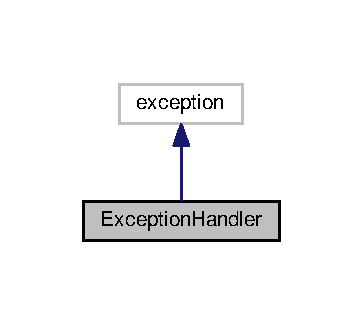
\includegraphics[width=174pt]{class_exception_handler__inherit__graph}
\end{center}
\end{figure}


Diagrama de colaboración para Exception\+Handler\+:\nopagebreak
\begin{figure}[H]
\begin{center}
\leavevmode
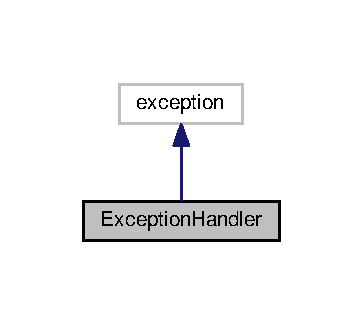
\includegraphics[width=174pt]{class_exception_handler__coll__graph}
\end{center}
\end{figure}
\subsection*{Métodos públicos}
\begin{DoxyCompactItemize}
\item 
\hyperlink{class_exception_handler_aad6e0ff56665a5e0576450c926fe227c}{Exception\+Handler} (const char $\ast$in\+Msg)
\begin{DoxyCompactList}\small\item\em Constructora con valor de inicialización. \end{DoxyCompactList}\item 
const char $\ast$ \hyperlink{class_exception_handler_a0ea814f22127aaa1f140343fd0077775}{what} () const   throw ()
\begin{DoxyCompactList}\small\item\em Consultor de motivo de excepción. \end{DoxyCompactList}\end{DoxyCompactItemize}


\subsection{Descripción detallada}
Controla la generación de excepciones en caso de fallo de las condiciones básicas de funcionamiento del programa. 

\subsection{Documentación del constructor y destructor}
\index{Exception\+Handler@{Exception\+Handler}!Exception\+Handler@{Exception\+Handler}}
\index{Exception\+Handler@{Exception\+Handler}!Exception\+Handler@{Exception\+Handler}}
\subsubsection[{\texorpdfstring{Exception\+Handler(const char $\ast$in\+Msg)}{ExceptionHandler(const char *inMsg)}}]{\setlength{\rightskip}{0pt plus 5cm}Exception\+Handler\+::\+Exception\+Handler (
\begin{DoxyParamCaption}
\item[{const char $\ast$}]{in\+Msg}
\end{DoxyParamCaption}
)\hspace{0.3cm}{\ttfamily [inline]}}\hypertarget{class_exception_handler_aad6e0ff56665a5e0576450c926fe227c}{}\label{class_exception_handler_aad6e0ff56665a5e0576450c926fe227c}


Constructora con valor de inicialización. 

\begin{DoxyPrecond}{Precondición}
{\itshape Cierto} 
\end{DoxyPrecond}
\begin{DoxyPostcond}{Postcondición}
Genera una excepción que muestra, si se proporciona, un mensaje por el canal estándar de salida de errores 
\end{DoxyPostcond}


\subsection{Documentación de las funciones miembro}
\index{Exception\+Handler@{Exception\+Handler}!what@{what}}
\index{what@{what}!Exception\+Handler@{Exception\+Handler}}
\subsubsection[{\texorpdfstring{what() const }{what() const }}]{\setlength{\rightskip}{0pt plus 5cm}const char$\ast$ Exception\+Handler\+::what (
\begin{DoxyParamCaption}
{}
\end{DoxyParamCaption}
) const throw  ) \hspace{0.3cm}{\ttfamily [inline]}}\hypertarget{class_exception_handler_a0ea814f22127aaa1f140343fd0077775}{}\label{class_exception_handler_a0ea814f22127aaa1f140343fd0077775}


Consultor de motivo de excepción. 

\begin{DoxyPrecond}{Precondición}
Se ha generado una excepción 
\end{DoxyPrecond}
\begin{DoxyPostcond}{Postcondición}
Devuelve el motivo por el que se ha generado la excepción, si se proporciona, contenido en el mensaje msg 
\end{DoxyPostcond}


La documentación para esta clase fue generada a partir del siguiente fichero\+:\begin{DoxyCompactItemize}
\item 
\hyperlink{_exception_handler_8hh}{Exception\+Handler.\+hh}\end{DoxyCompactItemize}

\hypertarget{class_expression}{}\section{Referencia de la Clase Expression}
\label{class_expression}\index{Expression@{Expression}}


Representa una expresión mediante el resultado de evaluarla, ya sea expresión entera, lista de expresiones enteras o indefinida.  


\subsection*{Métodos públicos}
\begin{DoxyCompactItemize}
\item 
\hyperlink{class_expression_afcf87716bf0abfe8d414c92529e1564a}{Expression} ()
\begin{DoxyCompactList}\small\item\em Constructora por defecto. \end{DoxyCompactList}\item 
\hyperlink{class_expression_ae84af9ba2a88741d6f65a70ef8869faf}{Expression} (const \hyperlink{class_expression}{Expression} \&in\+Exp)
\begin{DoxyCompactList}\small\item\em Constructora por copia. \end{DoxyCompactList}\item 
\hyperlink{class_expression_a3e99570b177da619eeb2c5787cbb148e}{$\sim$\+Expression} ()
\begin{DoxyCompactList}\small\item\em Destructora por defecto. \end{DoxyCompactList}\item 
\hyperlink{class_expression}{Expression} \& \hyperlink{class_expression_a674ab908807d385df298e12762e4220a}{operator=} (const \hyperlink{class_expression}{Expression} \&in\+Exp)
\begin{DoxyCompactList}\small\item\em Operación de asignación por copia. \end{DoxyCompactList}\item 
\hyperlink{class_expression}{Expression} \& \hyperlink{class_expression_a39021db3a461adc4e2b46c55ffd0e991}{operator$<$$<$} (\hyperlink{class_expression}{Expression} \&in\+Exp)
\begin{DoxyCompactList}\small\item\em Operación de asignación por transferencia. \end{DoxyCompactList}\item 
\hyperlink{class_expression}{Expression} \& \hyperlink{class_expression_a79f76778966b233f97217ed5c2cdefde}{operator$<$$<$} (list$<$ \hyperlink{class_expression}{Expression} $\ast$ $>$ \&l\+Expression)
\begin{DoxyCompactList}\small\item\em Operación de asignación de lista de expresiones por transferencia. \end{DoxyCompactList}\item 
void \hyperlink{class_expression_a21a202129abc628e19cebc38ad532dcc}{operator$>$$>$} (list$<$ \hyperlink{class_expression}{Expression} $\ast$ $>$ \&l\+Expression)
\begin{DoxyCompactList}\small\item\em Operación de asignación de lista de expresiones por transferencia. \end{DoxyCompactList}\item 
bool \hyperlink{class_expression_a8cd982884bef615b9c79526dce0956f6}{operator==} (const \hyperlink{class_expression}{Expression} \&in\+Exp) const 
\begin{DoxyCompactList}\small\item\em Operación de comparación de igualdad. \end{DoxyCompactList}\item 
bool \hyperlink{class_expression_a4f1f64418752d14e116f55b7b57355b8}{operator$<$} (const \hyperlink{class_expression}{Expression} \&in\+Exp) const 
\begin{DoxyCompactList}\small\item\em Operación de comparación lexicográfica de inferioridad exclusiva. \end{DoxyCompactList}\item 
void \hyperlink{class_expression_ab2e0ccb0146cccd559c39f8913f9585e}{clear} ()
\begin{DoxyCompactList}\small\item\em Operación de vaciado de expresión. \end{DoxyCompactList}\item 
void \hyperlink{class_expression_a2f087974bb5cee7d0ea06838f5d68ba8}{insert} (list$<$ \hyperlink{class_expression}{Expression} $\ast$ $>$\+::iterator it, \hyperlink{class_expression}{Expression} $\ast$p\+Exp)
\begin{DoxyCompactList}\small\item\em Operación de inserción de elemetos de lista. \end{DoxyCompactList}\item 
list$<$ \hyperlink{class_expression}{Expression} $\ast$ $>$\+::iterator \hyperlink{class_expression_a3fcf4ce4c5efde7795a6b3b004abf0ad}{erase} (list$<$ \hyperlink{class_expression}{Expression} $\ast$ $>$\+::iterator it)
\begin{DoxyCompactList}\small\item\em Operación de borrado de elemetos de lista. \end{DoxyCompactList}\item 
void \hyperlink{class_expression_afcd885fc3562809ede2796b722bb4854}{splice} (list$<$ \hyperlink{class_expression}{Expression} $\ast$ $>$\+::iterator it, list$<$ \hyperlink{class_expression}{Expression} $\ast$ $>$ l\+Expression)
\begin{DoxyCompactList}\small\item\em Operación de empalmado de listas. \end{DoxyCompactList}\item 
void \hyperlink{class_expression_a1668a7770489da5f57801254c35557ee}{swap\+\_\+list} (\hyperlink{class_expression}{Expression} \&in\+Exp)
\begin{DoxyCompactList}\small\item\em Operación de cambio de listas. \end{DoxyCompactList}\item 
void \hyperlink{class_expression_a1d3ddfe83d20f47930792807e8b22248}{set\+\_\+undefined} ()
\begin{DoxyCompactList}\small\item\em Modificadora a expresión indefinida. \end{DoxyCompactList}\item 
void \hyperlink{class_expression_a307683cc3735bf81d823931aab2d64e0}{set\+\_\+value} (int value)
\begin{DoxyCompactList}\small\item\em Modificadora de valor por asignación. \end{DoxyCompactList}\item 
void \hyperlink{class_expression_adffd3a10200510c64055e550e9eebb1f}{set\+\_\+op} (string \hyperlink{class_expression_a30856695b46075ada151f6f6cdfb9fa8}{op})
\begin{DoxyCompactList}\small\item\em Modificadora de operador. \end{DoxyCompactList}\item 
void \hyperlink{class_expression_a66db516be4fa87d58df4806938676508}{set\+\_\+list} ()
\begin{DoxyCompactList}\small\item\em Modificadora de lista. \end{DoxyCompactList}\item 
void \hyperlink{class_expression_a1e0ff9e6ef7b9b96466300509decab24}{set\+\_\+empty\+\_\+list} ()
\begin{DoxyCompactList}\small\item\em Modificadora de lista vacía. \end{DoxyCompactList}\item 
int \hyperlink{class_expression_a0e8980139631cf7bc9fd3bca9d8caddc}{size} () const 
\begin{DoxyCompactList}\small\item\em Consultora de tamaño de lista. \end{DoxyCompactList}\item 
bool \hyperlink{class_expression_a97f9b6fc78a7ef17dd9595e53a9b6239}{undefined} () const 
\begin{DoxyCompactList}\small\item\em Consultora de estado. \end{DoxyCompactList}\item 
bool \hyperlink{class_expression_a0020daf119d82799da034fd0513ca614}{empty} () const 
\begin{DoxyCompactList}\small\item\em Consultora de estado. \end{DoxyCompactList}\item 
bool \hyperlink{class_expression_a4ee60df2f212d8a4cc228ce7db2da81b}{is\+\_\+value} () const 
\begin{DoxyCompactList}\small\item\em Consultora de tipo de expresión variable. \end{DoxyCompactList}\item 
bool \hyperlink{class_expression_a422fb496720b177eaed37a9694613384}{is\+\_\+op} () const 
\begin{DoxyCompactList}\small\item\em Consultora de tipo de expresión operación. \end{DoxyCompactList}\item 
bool \hyperlink{class_expression_ae835c069faf7d6821fe6037e384f02c0}{is\+\_\+list} () const 
\begin{DoxyCompactList}\small\item\em Consultora de tipo de expresión lista. \end{DoxyCompactList}\item 
bool \hyperlink{class_expression_a776684354326520add7a3ca54a14f4f8}{is\+\_\+empty\+\_\+list} () const 
\begin{DoxyCompactList}\small\item\em Consultora de tipo de expresión lista vacía. \end{DoxyCompactList}\item 
bool \hyperlink{class_expression_ad42c70dcee3b195c77749ca6435c244d}{is\+\_\+bool} () const 
\begin{DoxyCompactList}\small\item\em Consultora de tipo de expresión booleana. \end{DoxyCompactList}\item 
int \hyperlink{class_expression_add3f908cb67ed993a5e886447fd70df0}{get\+\_\+value} () const 
\begin{DoxyCompactList}\small\item\em Consultora de valor. \end{DoxyCompactList}\item 
string \hyperlink{class_expression_a9216cba5bbd3ffa8c3a625a66b91b36f}{get\+\_\+op} () const 
\begin{DoxyCompactList}\small\item\em Consultora de operador. \end{DoxyCompactList}\item 
list$<$ \hyperlink{class_expression}{Expression} $\ast$ $>$\+::iterator \hyperlink{class_expression_a0ed7767d72f93c9121bb73afead5782a}{begin} ()
\begin{DoxyCompactList}\small\item\em Iterador de inicio de lista. \end{DoxyCompactList}\item 
list$<$ \hyperlink{class_expression}{Expression} $\ast$ $>$\+::const\+\_\+iterator \hyperlink{class_expression_a56b9a73d1c5f9b4c1a8a03d639e93ccb}{begin} () const 
\begin{DoxyCompactList}\small\item\em Iterador constante de inicio de lista. \end{DoxyCompactList}\item 
list$<$ \hyperlink{class_expression}{Expression} $\ast$ $>$\+::iterator \hyperlink{class_expression_ae53f7febf676d564d6393bf2762fc08e}{second} ()
\begin{DoxyCompactList}\small\item\em Iterador de segundo elemento de lista. \end{DoxyCompactList}\item 
list$<$ \hyperlink{class_expression}{Expression} $\ast$ $>$\+::const\+\_\+iterator \hyperlink{class_expression_a9991190559b6d1cc04e3b6fc2ade7b18}{second} () const 
\begin{DoxyCompactList}\small\item\em Iterador constante de segundo elemento de lista. \end{DoxyCompactList}\item 
list$<$ \hyperlink{class_expression}{Expression} $\ast$ $>$\+::iterator \hyperlink{class_expression_af5229aaf6bbb7200db55f220f315192e}{end} ()
\begin{DoxyCompactList}\small\item\em Iterador de final de lista. \end{DoxyCompactList}\item 
list$<$ \hyperlink{class_expression}{Expression} $\ast$ $>$\+::const\+\_\+iterator \hyperlink{class_expression_aa8be0d8b3dc53907a982c18e0c159b49}{end} () const 
\begin{DoxyCompactList}\small\item\em Iterador constante de final de lista. \end{DoxyCompactList}\item 
void \hyperlink{class_expression_a6d5d0fa496e3713c332c9f1edc269de5}{write} () const 
\begin{DoxyCompactList}\small\item\em Operación de escritura de expresión. \end{DoxyCompactList}\end{DoxyCompactItemize}
\subsection*{Métodos privados estáticos}
\begin{DoxyCompactItemize}
\item 
static list$<$ \hyperlink{class_expression}{Expression} $\ast$ $>$ \hyperlink{class_expression_a0d7df919d94bc861a5fe5be4be2dc836}{cp\+\_\+exp\+\_\+list} (const list$<$ \hyperlink{class_expression}{Expression} $\ast$ $>$ \&\hyperlink{class_expression_afb4f4617291f7e182cbf2252151b122a}{l\+Exp})
\begin{DoxyCompactList}\small\item\em Método privado de copia de lista de expresiones. \end{DoxyCompactList}\item 
static void \hyperlink{class_expression_ae80247fcce0b4d61f7b0227d5e176dce}{rm\+\_\+exp\+\_\+list} (list$<$ \hyperlink{class_expression}{Expression} $\ast$ $>$ \&\hyperlink{class_expression_afb4f4617291f7e182cbf2252151b122a}{l\+Exp})
\begin{DoxyCompactList}\small\item\em Método privado de borrado de lista de expresiones. \end{DoxyCompactList}\item 
static void \hyperlink{class_expression_af84a5a0c390b2cd9f481ed6e0a894d60}{rm\+\_\+exp\+\_\+list\+\_\+excep} (list$<$ \hyperlink{class_expression}{Expression} $\ast$ $>$ \&\hyperlink{class_expression_afb4f4617291f7e182cbf2252151b122a}{l\+Exp}, \hyperlink{class_expression}{Expression} \&in\+Exp)
\begin{DoxyCompactList}\small\item\em Método privado de borrado de lista de expresiones con excepción. \end{DoxyCompactList}\end{DoxyCompactItemize}
\subsection*{Atributos privados}
\begin{DoxyCompactItemize}
\item 
unsigned char \hyperlink{class_expression_a2c094b93c4863b1f851ea2136aae9612}{type}
\begin{DoxyCompactList}\small\item\em Tipo de expresión. \end{DoxyCompactList}\item 
int \hyperlink{class_expression_a9c15b529b5d59e6bffb3855e384c04aa}{val}
\begin{DoxyCompactList}\small\item\em Valor de expresión. \end{DoxyCompactList}\item 
string \hyperlink{class_expression_a30856695b46075ada151f6f6cdfb9fa8}{op}
\begin{DoxyCompactList}\small\item\em Operador. \end{DoxyCompactList}\item 
list$<$ \hyperlink{class_expression}{Expression} $\ast$ $>$ \hyperlink{class_expression_afb4f4617291f7e182cbf2252151b122a}{l\+Exp}
\begin{DoxyCompactList}\small\item\em Lista de expresiones. \end{DoxyCompactList}\end{DoxyCompactItemize}


\subsection{Descripción detallada}
Representa una expresión mediante el resultado de evaluarla, ya sea expresión entera, lista de expresiones enteras o indefinida. 

Definición en la línea 19 del archivo Expression.\+hh.



\subsection{Documentación del constructor y destructor}
\index{Expression@{Expression}!Expression@{Expression}}
\index{Expression@{Expression}!Expression@{Expression}}
\subsubsection[{\texorpdfstring{Expression()}{Expression()}}]{\setlength{\rightskip}{0pt plus 5cm}Expression\+::\+Expression (
\begin{DoxyParamCaption}
{}
\end{DoxyParamCaption}
)}\hypertarget{class_expression_afcf87716bf0abfe8d414c92529e1564a}{}\label{class_expression_afcf87716bf0abfe8d414c92529e1564a}


Constructora por defecto. 

Se ejecuta automáticamente al declarar una nueva expresión \begin{DoxyPrecond}{Precondición}
{\itshape Cierto} 
\end{DoxyPrecond}
\begin{DoxyPostcond}{Postcondición}
Crea un objeto vacío 
\end{DoxyPostcond}
\begin{DoxyParagraph}{Coste}
Constante 
\end{DoxyParagraph}


Definición en la línea 57 del archivo Expression.\+cc.


\begin{DoxyCode}
58 \{
59   \hyperlink{class_expression_a2c094b93c4863b1f851ea2136aae9612}{type} = 1;
60 \}
\end{DoxyCode}
\index{Expression@{Expression}!Expression@{Expression}}
\index{Expression@{Expression}!Expression@{Expression}}
\subsubsection[{\texorpdfstring{Expression(const Expression \&in\+Exp)}{Expression(const Expression &inExp)}}]{\setlength{\rightskip}{0pt plus 5cm}Expression\+::\+Expression (
\begin{DoxyParamCaption}
\item[{const {\bf Expression} \&}]{in\+Exp}
\end{DoxyParamCaption}
)}\hypertarget{class_expression_ae84af9ba2a88741d6f65a70ef8869faf}{}\label{class_expression_ae84af9ba2a88741d6f65a70ef8869faf}


Constructora por copia. 

\begin{DoxyPrecond}{Precondición}
{\itshape Cierto} 
\end{DoxyPrecond}
\begin{DoxyPostcond}{Postcondición}
Crea un objeto copia de \textquotesingle{}in\+Exp\textquotesingle{} 
\end{DoxyPostcond}
\begin{DoxyParagraph}{Coste}
Lineal respecto al tamaño de \textquotesingle{}in\+Exp\textquotesingle{} 
\end{DoxyParagraph}


Definición en la línea 62 del archivo Expression.\+cc.


\begin{DoxyCode}
63 \{
64   \hyperlink{class_expression_a2c094b93c4863b1f851ea2136aae9612}{type} = inExp.\hyperlink{class_expression_a2c094b93c4863b1f851ea2136aae9612}{type};
65   \hyperlink{class_expression_a9c15b529b5d59e6bffb3855e384c04aa}{val} = inExp.\hyperlink{class_expression_a9c15b529b5d59e6bffb3855e384c04aa}{val};
66   \hyperlink{class_expression_a30856695b46075ada151f6f6cdfb9fa8}{op} = inExp.\hyperlink{class_expression_a30856695b46075ada151f6f6cdfb9fa8}{op};
67   \hyperlink{class_expression_afb4f4617291f7e182cbf2252151b122a}{lExp} = \hyperlink{class_expression_a0d7df919d94bc861a5fe5be4be2dc836}{cp\_exp\_list}(inExp.\hyperlink{class_expression_afb4f4617291f7e182cbf2252151b122a}{lExp});
68 \}
\end{DoxyCode}
\index{Expression@{Expression}!````~Expression@{$\sim$\+Expression}}
\index{````~Expression@{$\sim$\+Expression}!Expression@{Expression}}
\subsubsection[{\texorpdfstring{$\sim$\+Expression()}{~Expression()}}]{\setlength{\rightskip}{0pt plus 5cm}Expression\+::$\sim$\+Expression (
\begin{DoxyParamCaption}
{}
\end{DoxyParamCaption}
)}\hypertarget{class_expression_a3e99570b177da619eeb2c5787cbb148e}{}\label{class_expression_a3e99570b177da619eeb2c5787cbb148e}


Destructora por defecto. 

Se ejecuta automáticamente al salir de un ámbito de visibilidad \begin{DoxyPrecond}{Precondición}
{\itshape Cierto} 
\end{DoxyPrecond}
\begin{DoxyPostcond}{Postcondición}
Libera los recursos locales del parámetro implícito al salir de un ámbito de visibilidad 
\end{DoxyPostcond}
\begin{DoxyParagraph}{Coste}
Lineal respecto al tamaño de la lista de expresiones del parámetro implícito 
\end{DoxyParagraph}


Definición en la línea 72 del archivo Expression.\+cc.


\begin{DoxyCode}
73 \{
74   \hyperlink{class_expression_ae80247fcce0b4d61f7b0227d5e176dce}{rm\_exp\_list}(\hyperlink{class_expression_afb4f4617291f7e182cbf2252151b122a}{lExp});
75 \}
\end{DoxyCode}


\subsection{Documentación de las funciones miembro}
\index{Expression@{Expression}!cp\+\_\+exp\+\_\+list@{cp\+\_\+exp\+\_\+list}}
\index{cp\+\_\+exp\+\_\+list@{cp\+\_\+exp\+\_\+list}!Expression@{Expression}}
\subsubsection[{\texorpdfstring{cp\+\_\+exp\+\_\+list(const list$<$ Expression $\ast$ $>$ \&l\+Exp)}{cp_exp_list(const list< Expression * > &lExp)}}]{\setlength{\rightskip}{0pt plus 5cm}list$<$ {\bf Expression} $\ast$ $>$ Expression\+::cp\+\_\+exp\+\_\+list (
\begin{DoxyParamCaption}
\item[{const list$<$ {\bf Expression} $\ast$ $>$ \&}]{l\+Exp}
\end{DoxyParamCaption}
)\hspace{0.3cm}{\ttfamily [static]}, {\ttfamily [private]}}\hypertarget{class_expression_a0d7df919d94bc861a5fe5be4be2dc836}{}\label{class_expression_a0d7df919d94bc861a5fe5be4be2dc836}


Método privado de copia de lista de expresiones. 

\begin{DoxyPrecond}{Precondición}
{\itshape Cierto} 
\end{DoxyPrecond}
\begin{DoxyPostcond}{Postcondición}
Devuelve una lista de punteros que apuntan a una copia en memoria de los objetos apuntados por \textquotesingle{}l\+Exp\textquotesingle{}, es decir, devuelve una lista conteniendo una copia del contenido de la lista \textquotesingle{}l\+Exp\textquotesingle{} 
\end{DoxyPostcond}
\begin{DoxyParagraph}{Coste}
Lineal respecto al tamaño de \textquotesingle{}l\+Exp\textquotesingle{} 
\end{DoxyParagraph}


Definición en la línea 15 del archivo Expression.\+cc.


\begin{DoxyCode}
16 \{
17   list<Expression*> aux;
18   \hyperlink{class_expression}{Expression}* pAux;
19   \hyperlink{_expression_8cc_a6ff59711533978050143f1bfb54c33b1}{const\_iter} c\_it = \hyperlink{class_expression_afb4f4617291f7e182cbf2252151b122a}{lExp}.begin();
20   \textcolor{comment}{/* INV}
21 \textcolor{comment}{    c\_it es un iterador a un elemento de la lista de expresiones del parámetro implícito comprendido entre
       lExp.begin() y lExp.end()}
22 \textcolor{comment}{  */}
23   \textcolor{keywordflow}{while}(c\_it != \hyperlink{class_expression_afb4f4617291f7e182cbf2252151b122a}{lExp}.end())\{
24     pAux = \textcolor{keyword}{new} \hyperlink{class_expression_afcf87716bf0abfe8d414c92529e1564a}{Expression};
25     pAux -> \hyperlink{class_expression_a2c094b93c4863b1f851ea2136aae9612}{type} = (*c\_it) -> \hyperlink{class_expression_a2c094b93c4863b1f851ea2136aae9612}{type};
26     pAux -> \hyperlink{class_expression_a9c15b529b5d59e6bffb3855e384c04aa}{val} = (*c\_it) -> \hyperlink{class_expression_a9c15b529b5d59e6bffb3855e384c04aa}{val};
27     pAux -> \hyperlink{class_expression_a30856695b46075ada151f6f6cdfb9fa8}{op} = (*c\_it) -> \hyperlink{class_expression_a30856695b46075ada151f6f6cdfb9fa8}{op};
28     \textcolor{comment}{/* HI}
29 \textcolor{comment}{      cp\_exp\_list devuelve una lista de punteros que apuntan a una copia en memoria de los objetos
       apuntados por la lista pasada como parámetro}
30 \textcolor{comment}{    */}
31     pAux -> \hyperlink{class_expression_afb4f4617291f7e182cbf2252151b122a}{lExp} = \hyperlink{class_expression_a0d7df919d94bc861a5fe5be4be2dc836}{cp\_exp\_list}((*c\_it) -> \hyperlink{class_expression_afb4f4617291f7e182cbf2252151b122a}{lExp});
32     aux.insert(aux.end(), pAux);
33     ++c\_it;
34   \}
35   \textcolor{keywordflow}{return} aux;
36 \}
\end{DoxyCode}
\index{Expression@{Expression}!rm\+\_\+exp\+\_\+list@{rm\+\_\+exp\+\_\+list}}
\index{rm\+\_\+exp\+\_\+list@{rm\+\_\+exp\+\_\+list}!Expression@{Expression}}
\subsubsection[{\texorpdfstring{rm\+\_\+exp\+\_\+list(list$<$ Expression $\ast$ $>$ \&l\+Exp)}{rm_exp_list(list< Expression * > &lExp)}}]{\setlength{\rightskip}{0pt plus 5cm}void Expression\+::rm\+\_\+exp\+\_\+list (
\begin{DoxyParamCaption}
\item[{list$<$ {\bf Expression} $\ast$ $>$ \&}]{l\+Exp}
\end{DoxyParamCaption}
)\hspace{0.3cm}{\ttfamily [static]}, {\ttfamily [private]}}\hypertarget{class_expression_ae80247fcce0b4d61f7b0227d5e176dce}{}\label{class_expression_ae80247fcce0b4d61f7b0227d5e176dce}


Método privado de borrado de lista de expresiones. 

\begin{DoxyPrecond}{Precondición}
{\itshape Cierto} 
\end{DoxyPrecond}
\begin{DoxyPostcond}{Postcondición}
Elimina todos los elementos apuntados por la lista \textquotesingle{}l\+Exp\textquotesingle{} y libera la memoria ocupada por ellos 
\end{DoxyPostcond}
\begin{DoxyParagraph}{Coste}
Lineal respecto al tamaño de \textquotesingle{}l\+Exp\textquotesingle{} 
\end{DoxyParagraph}


Definición en la línea 38 del archivo Expression.\+cc.


\begin{DoxyCode}
39 \{
40   \textcolor{keywordflow}{for} (\hyperlink{_expression_8cc_a1d50eb14ec5470381cccafb7dcd8b687}{iter} it = \hyperlink{class_expression_afb4f4617291f7e182cbf2252151b122a}{lExp}.begin(); it != \hyperlink{class_expression_afb4f4617291f7e182cbf2252151b122a}{lExp}.end(); ++it) \{
41     \textcolor{keywordflow}{if}(*it != \hyperlink{_expression_8cc_a67b562dac02b0d19c41323121556d04b}{rm\_excep})\{
42       \textcolor{keyword}{delete} *it;
43     \}
44   \}
45   \hyperlink{class_expression_afb4f4617291f7e182cbf2252151b122a}{lExp}.clear();
46 \}
\end{DoxyCode}
\index{Expression@{Expression}!rm\+\_\+exp\+\_\+list\+\_\+excep@{rm\+\_\+exp\+\_\+list\+\_\+excep}}
\index{rm\+\_\+exp\+\_\+list\+\_\+excep@{rm\+\_\+exp\+\_\+list\+\_\+excep}!Expression@{Expression}}
\subsubsection[{\texorpdfstring{rm\+\_\+exp\+\_\+list\+\_\+excep(list$<$ Expression $\ast$ $>$ \&l\+Exp, Expression \&in\+Exp)}{rm_exp_list_excep(list< Expression * > &lExp, Expression &inExp)}}]{\setlength{\rightskip}{0pt plus 5cm}void Expression\+::rm\+\_\+exp\+\_\+list\+\_\+excep (
\begin{DoxyParamCaption}
\item[{list$<$ {\bf Expression} $\ast$ $>$ \&}]{l\+Exp, }
\item[{{\bf Expression} \&}]{in\+Exp}
\end{DoxyParamCaption}
)\hspace{0.3cm}{\ttfamily [static]}, {\ttfamily [private]}}\hypertarget{class_expression_af84a5a0c390b2cd9f481ed6e0a894d60}{}\label{class_expression_af84a5a0c390b2cd9f481ed6e0a894d60}


Método privado de borrado de lista de expresiones con excepción. 

\begin{DoxyPrecond}{Precondición}
{\itshape Cierto} 
\end{DoxyPrecond}
\begin{DoxyPostcond}{Postcondición}
Elimina todos los elementos apuntados por la lista \textquotesingle{}l\+Expression\textquotesingle{} a excepción del elemento \textquotesingle{}in\+Exp\textquotesingle{} y todos los que dependen de él (si forma parte de \textquotesingle{}l\+Exp\textquotesingle{} o de alguno de los elementos apuntados por los elementos de \textquotesingle{}l\+Exp\textquotesingle{}), y libera la memoria ocupada por ellos 
\end{DoxyPostcond}
\begin{DoxyParagraph}{Coste}
Lineal respecto al tamaño de \textquotesingle{}l\+Exp\textquotesingle{} 
\end{DoxyParagraph}


Definición en la línea 48 del archivo Expression.\+cc.


\begin{DoxyCode}
49 \{
50     \hyperlink{_expression_8cc_a67b562dac02b0d19c41323121556d04b}{rm\_excep} = &inExp;
51     \hyperlink{class_expression_ae80247fcce0b4d61f7b0227d5e176dce}{rm\_exp\_list}(\hyperlink{class_expression_afb4f4617291f7e182cbf2252151b122a}{lExp});
52     \hyperlink{_expression_8cc_a67b562dac02b0d19c41323121556d04b}{rm\_excep} = NULL;
53 \}
\end{DoxyCode}
\index{Expression@{Expression}!operator=@{operator=}}
\index{operator=@{operator=}!Expression@{Expression}}
\subsubsection[{\texorpdfstring{operator=(const Expression \&in\+Exp)}{operator=(const Expression &inExp)}}]{\setlength{\rightskip}{0pt plus 5cm}{\bf Expression} \& Expression\+::operator= (
\begin{DoxyParamCaption}
\item[{const {\bf Expression} \&}]{in\+Exp}
\end{DoxyParamCaption}
)}\hypertarget{class_expression_a674ab908807d385df298e12762e4220a}{}\label{class_expression_a674ab908807d385df298e12762e4220a}


Operación de asignación por copia. 

\begin{DoxyPrecond}{Precondición}
{\itshape Cierto} 
\end{DoxyPrecond}
\begin{DoxyPostcond}{Postcondición}
El parámetro implícito pasa a ser una copia de \textquotesingle{}in\+Exp\textquotesingle{}; retorna el parámetro implícito 
\end{DoxyPostcond}
\begin{DoxyParagraph}{Coste}
Lineal respecto al tamaño de \textquotesingle{}in\+Exp\textquotesingle{} 
\end{DoxyParagraph}


Definición en la línea 79 del archivo Expression.\+cc.


\begin{DoxyCode}
80 \{
81   \textcolor{keywordflow}{if}(\textcolor{keyword}{this} != &inExp) \{
82     \hyperlink{class_expression_a2c094b93c4863b1f851ea2136aae9612}{type} = inExp.\hyperlink{class_expression_a2c094b93c4863b1f851ea2136aae9612}{type};
83     \hyperlink{class_expression_a9c15b529b5d59e6bffb3855e384c04aa}{val} = inExp.\hyperlink{class_expression_a9c15b529b5d59e6bffb3855e384c04aa}{val};
84     \hyperlink{class_expression_a30856695b46075ada151f6f6cdfb9fa8}{op} = inExp.\hyperlink{class_expression_a30856695b46075ada151f6f6cdfb9fa8}{op};
85     list<Expression*> aux = \hyperlink{class_expression_a0d7df919d94bc861a5fe5be4be2dc836}{cp\_exp\_list}(inExp.\hyperlink{class_expression_afb4f4617291f7e182cbf2252151b122a}{lExp});
86     \hyperlink{class_expression_ae80247fcce0b4d61f7b0227d5e176dce}{rm\_exp\_list}(\hyperlink{class_expression_afb4f4617291f7e182cbf2252151b122a}{lExp});
87     \hyperlink{class_expression_afb4f4617291f7e182cbf2252151b122a}{lExp} = aux;
88   \}
89   \textcolor{keywordflow}{return} *\textcolor{keyword}{this};
90 \}
\end{DoxyCode}
\index{Expression@{Expression}!operator$<$$<$@{operator$<$$<$}}
\index{operator$<$$<$@{operator$<$$<$}!Expression@{Expression}}
\subsubsection[{\texorpdfstring{operator$<$$<$(\+Expression \&in\+Exp)}{operator<<(Expression &inExp)}}]{\setlength{\rightskip}{0pt plus 5cm}{\bf Expression} \& Expression\+::operator$<$$<$ (
\begin{DoxyParamCaption}
\item[{{\bf Expression} \&}]{in\+Exp}
\end{DoxyParamCaption}
)}\hypertarget{class_expression_a39021db3a461adc4e2b46c55ffd0e991}{}\label{class_expression_a39021db3a461adc4e2b46c55ffd0e991}


Operación de asignación por transferencia. 

\begin{DoxyPrecond}{Precondición}
{\itshape Cierto} 
\end{DoxyPrecond}
\begin{DoxyPostcond}{Postcondición}
El parámetro implícito pasa a tener todos los elementos de \textquotesingle{}in\+Exp\textquotesingle{} mediante transferencia (sin reubicación de datos en memoria); \textquotesingle{}in\+Exp\textquotesingle{} pasa a dejar de existir en memoria; retorna el parámetro implícito 
\end{DoxyPostcond}
\begin{DoxyParagraph}{Coste}
Lineal respecto al tamaño de \textquotesingle{}in\+Exp\textquotesingle{} 
\end{DoxyParagraph}


Definición en la línea 92 del archivo Expression.\+cc.


\begin{DoxyCode}
93 \{
94   \textcolor{keywordflow}{if}(\textcolor{keyword}{this} != &inExp)\{
95     \hyperlink{class_expression_a2c094b93c4863b1f851ea2136aae9612}{type} = inExp.\hyperlink{class_expression_a2c094b93c4863b1f851ea2136aae9612}{type};
96     \hyperlink{class_expression_a9c15b529b5d59e6bffb3855e384c04aa}{val} = inExp.\hyperlink{class_expression_a9c15b529b5d59e6bffb3855e384c04aa}{val};
97     \hyperlink{class_expression_a30856695b46075ada151f6f6cdfb9fa8}{op} = inExp.\hyperlink{class_expression_a30856695b46075ada151f6f6cdfb9fa8}{op};
98     \hyperlink{class_expression_af84a5a0c390b2cd9f481ed6e0a894d60}{rm\_exp\_list\_excep}(\hyperlink{class_expression_afb4f4617291f7e182cbf2252151b122a}{lExp}, inExp);
99     \hyperlink{class_expression_afb4f4617291f7e182cbf2252151b122a}{lExp} = inExp.\hyperlink{class_expression_afb4f4617291f7e182cbf2252151b122a}{lExp};
100     inExp.\hyperlink{class_expression_afb4f4617291f7e182cbf2252151b122a}{lExp}.clear();
101     inExp.\hyperlink{class_expression_ab2e0ccb0146cccd559c39f8913f9585e}{clear}();
102     \textcolor{keyword}{delete} &inExp;
103   \}
104   \textcolor{keywordflow}{return} *\textcolor{keyword}{this};
105 \}
\end{DoxyCode}
\index{Expression@{Expression}!operator$<$$<$@{operator$<$$<$}}
\index{operator$<$$<$@{operator$<$$<$}!Expression@{Expression}}
\subsubsection[{\texorpdfstring{operator$<$$<$(list$<$ Expression $\ast$ $>$ \&l\+Expression)}{operator<<(list< Expression * > &lExpression)}}]{\setlength{\rightskip}{0pt plus 5cm}{\bf Expression} \& Expression\+::operator$<$$<$ (
\begin{DoxyParamCaption}
\item[{list$<$ {\bf Expression} $\ast$ $>$ \&}]{l\+Expression}
\end{DoxyParamCaption}
)}\hypertarget{class_expression_a79f76778966b233f97217ed5c2cdefde}{}\label{class_expression_a79f76778966b233f97217ed5c2cdefde}


Operación de asignación de lista de expresiones por transferencia. 

\begin{DoxyPrecond}{Precondición}
{\itshape Cierto} 
\end{DoxyPrecond}
\begin{DoxyPostcond}{Postcondición}
El parámetro implícito pasa a tener la lista de expresiones de \textquotesingle{}l\+Expression\textquotesingle{} mediante transferencia (sin reubicación de datos en memoria); \textquotesingle{}l\+Expression\textquotesingle{} pasa a estar vacía; retorna el parámetro implícito 
\end{DoxyPostcond}
\begin{DoxyParagraph}{Coste}
Lineal respecto al tamaño de \textquotesingle{}l\+Expression\textquotesingle{} 
\end{DoxyParagraph}


Definición en la línea 107 del archivo Expression.\+cc.


\begin{DoxyCode}
108 \{
109   \hyperlink{class_expression_ae80247fcce0b4d61f7b0227d5e176dce}{rm\_exp\_list}(\hyperlink{class_expression_afb4f4617291f7e182cbf2252151b122a}{lExp});
110   \hyperlink{class_expression_afb4f4617291f7e182cbf2252151b122a}{lExp} = lExpression;
111   lExpression.clear();
112   \textcolor{keywordflow}{return} *\textcolor{keyword}{this};
113 \}
\end{DoxyCode}
\index{Expression@{Expression}!operator$>$$>$@{operator$>$$>$}}
\index{operator$>$$>$@{operator$>$$>$}!Expression@{Expression}}
\subsubsection[{\texorpdfstring{operator$>$$>$(list$<$ Expression $\ast$ $>$ \&l\+Expression)}{operator>>(list< Expression * > &lExpression)}}]{\setlength{\rightskip}{0pt plus 5cm}void Expression\+::operator$>$$>$ (
\begin{DoxyParamCaption}
\item[{list$<$ {\bf Expression} $\ast$ $>$ \&}]{l\+Expression}
\end{DoxyParamCaption}
)}\hypertarget{class_expression_a21a202129abc628e19cebc38ad532dcc}{}\label{class_expression_a21a202129abc628e19cebc38ad532dcc}


Operación de asignación de lista de expresiones por transferencia. 

\begin{DoxyPrecond}{Precondición}
{\itshape Cierto} 
\end{DoxyPrecond}
\begin{DoxyPostcond}{Postcondición}
La lista \textquotesingle{}l\+Expression\textquotesingle{} pasa a tener la lista de expresiones del parámetro implícito mediante transferencia (sin reubicación de datos en memoria); la lista del parámetro implícito pasa a estar vacía 
\end{DoxyPostcond}
\begin{DoxyParagraph}{Coste}
Lineal respecto al tamaño de \textquotesingle{}l\+Expression\textquotesingle{} 
\end{DoxyParagraph}


Definición en la línea 115 del archivo Expression.\+cc.


\begin{DoxyCode}
116 \{
117   \hyperlink{class_expression_ae80247fcce0b4d61f7b0227d5e176dce}{rm\_exp\_list}(lExpression);
118   lExpression = \hyperlink{class_expression_afb4f4617291f7e182cbf2252151b122a}{lExp};
119   \hyperlink{class_expression_afb4f4617291f7e182cbf2252151b122a}{lExp}.clear();
120 \}
\end{DoxyCode}
\index{Expression@{Expression}!operator==@{operator==}}
\index{operator==@{operator==}!Expression@{Expression}}
\subsubsection[{\texorpdfstring{operator==(const Expression \&in\+Exp) const }{operator==(const Expression &inExp) const }}]{\setlength{\rightskip}{0pt plus 5cm}bool Expression\+::operator== (
\begin{DoxyParamCaption}
\item[{const {\bf Expression} \&}]{in\+Exp}
\end{DoxyParamCaption}
) const}\hypertarget{class_expression_a8cd982884bef615b9c79526dce0956f6}{}\label{class_expression_a8cd982884bef615b9c79526dce0956f6}


Operación de comparación de igualdad. 

\begin{DoxyPrecond}{Precondición}
{\itshape Cierto} 
\end{DoxyPrecond}
\begin{DoxyPostcond}{Postcondición}
Si el parámetro implícito y \textquotesingle{}in\+Exp\textquotesingle{} son valores, devuelve cierto si son iguales; si ambos son listas de expresiones, devuelve cierto si los elementos de las respectivas posiciones de ambas listas son iguales; en otro caso, devuelve falso 
\end{DoxyPostcond}
\begin{DoxyParagraph}{Coste}
Lineal respecto al tamaño de \textquotesingle{}in\+Exp\textquotesingle{} 
\end{DoxyParagraph}


Definición en la línea 122 del archivo Expression.\+cc.


\begin{DoxyCode}
123 \{
124   \textcolor{keywordflow}{if}(\hyperlink{class_expression_a2c094b93c4863b1f851ea2136aae9612}{type} == 2 and inExp.\hyperlink{class_expression_a2c094b93c4863b1f851ea2136aae9612}{type} == 2) \{
125     \textcolor{keywordflow}{return} \hyperlink{class_expression_a9c15b529b5d59e6bffb3855e384c04aa}{val} == inExp.\hyperlink{class_expression_a9c15b529b5d59e6bffb3855e384c04aa}{val};
126   \}
127   \textcolor{keywordflow}{else} \textcolor{keywordflow}{if}(\hyperlink{class_expression_a2c094b93c4863b1f851ea2136aae9612}{type} == 4 and inExp.\hyperlink{class_expression_a2c094b93c4863b1f851ea2136aae9612}{type} == 4) \{
128     \textcolor{keywordflow}{if}(\hyperlink{class_expression_afb4f4617291f7e182cbf2252151b122a}{lExp}.size() == inExp.\hyperlink{class_expression_afb4f4617291f7e182cbf2252151b122a}{lExp}.size()) \{
129       \hyperlink{_expression_8cc_a6ff59711533978050143f1bfb54c33b1}{const\_iter} c\_it1 = \hyperlink{class_expression_afb4f4617291f7e182cbf2252151b122a}{lExp}.begin();
130       \hyperlink{_expression_8cc_a6ff59711533978050143f1bfb54c33b1}{const\_iter} c\_it2 = inExp.\hyperlink{class_expression_afb4f4617291f7e182cbf2252151b122a}{lExp}.begin();
131       \textcolor{comment}{/* INV}
132 \textcolor{comment}{        c\_it1 es un iterador a un elemento de la lista de expresiones del parámetro implícito comprendido
       entre lExp.begin() y lExp.end()}
133 \textcolor{comment}{        c\_it2 es un iterador a un elemento de la lista de expresiones de 'inExp' comprendido entre
       inExp.lExp.begin() y inExp.lExp.end()}
134 \textcolor{comment}{      */}
135       \textcolor{comment}{/* HI}
136 \textcolor{comment}{        *(*c\_it1) == *(*c\_it2) devuelve 'true' si ambas expresiones son iguales y 'false' en otro caso}
137 \textcolor{comment}{      */}
138       \textcolor{keywordflow}{while}(c\_it1 != \hyperlink{class_expression_afb4f4617291f7e182cbf2252151b122a}{lExp}.end() and (*(*c\_it1) == *(*c\_it2))) \{
139         ++c\_it1;
140         ++c\_it2;
141       \}
142       \textcolor{keywordflow}{return} c\_it1 == \hyperlink{class_expression_afb4f4617291f7e182cbf2252151b122a}{lExp}.end();
143     \}
144     \textcolor{keywordflow}{else} \{
145       \textcolor{keywordflow}{return} \textcolor{keyword}{false};
146     \}
147   \}
148   \textcolor{keywordflow}{else} \{
149     \textcolor{keywordflow}{return} \textcolor{keyword}{false};
150   \}
151 \}
\end{DoxyCode}
\index{Expression@{Expression}!operator$<$@{operator$<$}}
\index{operator$<$@{operator$<$}!Expression@{Expression}}
\subsubsection[{\texorpdfstring{operator$<$(const Expression \&in\+Exp) const }{operator<(const Expression &inExp) const }}]{\setlength{\rightskip}{0pt plus 5cm}bool Expression\+::operator$<$ (
\begin{DoxyParamCaption}
\item[{const {\bf Expression} \&}]{in\+Exp}
\end{DoxyParamCaption}
) const}\hypertarget{class_expression_a4f1f64418752d14e116f55b7b57355b8}{}\label{class_expression_a4f1f64418752d14e116f55b7b57355b8}


Operación de comparación lexicográfica de inferioridad exclusiva. 

\begin{DoxyPrecond}{Precondición}
{\itshape Cierto} 
\end{DoxyPrecond}
\begin{DoxyPostcond}{Postcondición}
Devuelve cierto si el parámetro implícito es lexicográficamente menor exclusivo que \textquotesingle{}in\+Exp\textquotesingle{} 
\end{DoxyPostcond}
\begin{DoxyParagraph}{Coste}
Lineal respecto al tamaño de \textquotesingle{}in\+Exp\textquotesingle{} 
\end{DoxyParagraph}


Definición en la línea 153 del archivo Expression.\+cc.


\begin{DoxyCode}
154 \{
155   \textcolor{keywordflow}{if}(\hyperlink{class_expression_a2c094b93c4863b1f851ea2136aae9612}{type} == 2 and inExp.\hyperlink{class_expression_a2c094b93c4863b1f851ea2136aae9612}{type} == 2) \{
156     \textcolor{keywordflow}{return} \hyperlink{class_expression_a9c15b529b5d59e6bffb3855e384c04aa}{val} < inExp.\hyperlink{class_expression_a9c15b529b5d59e6bffb3855e384c04aa}{val};
157   \}
158   \textcolor{keywordflow}{else} \textcolor{keywordflow}{if}(\hyperlink{class_expression_a2c094b93c4863b1f851ea2136aae9612}{type} == 4 and inExp.\hyperlink{class_expression_a2c094b93c4863b1f851ea2136aae9612}{type} == 4) \{
159     \hyperlink{_expression_8cc_a6ff59711533978050143f1bfb54c33b1}{const\_iter} c\_it1 = \hyperlink{class_expression_afb4f4617291f7e182cbf2252151b122a}{lExp}.begin();
160     \hyperlink{_expression_8cc_a6ff59711533978050143f1bfb54c33b1}{const\_iter} c\_it2 = inExp.\hyperlink{class_expression_afb4f4617291f7e182cbf2252151b122a}{lExp}.begin();
161     \textcolor{comment}{/* INV}
162 \textcolor{comment}{      c\_it1 es un iterador a un elemento de la lista de expresiones del parámetro implícito comprendido
       entre lExp.begin() y lExp.end()}
163 \textcolor{comment}{      c\_it2 es un iterador a un elemento de la lista de expresiones de 'inExp' comprendido entre
       inExp.lExp.begin() y inExp.lExp.end()}
164 \textcolor{comment}{    */}
165     \textcolor{keywordflow}{while}(c\_it1 != \hyperlink{class_expression_afb4f4617291f7e182cbf2252151b122a}{lExp}.end() and c\_it2 != inExp.\hyperlink{class_expression_afb4f4617291f7e182cbf2252151b122a}{lExp}.end() and (*(*c\_it1) == *(*c\_it2))) \{
166       ++c\_it1;
167       ++c\_it2;
168     \}
169     \textcolor{comment}{/* HI}
170 \textcolor{comment}{      *(*c\_it1) < *(*c\_it2)) devuelve 'true' si la expresión de la izquierda del operador es
       lexicográficamente menor estricta que la de la derecha del operador}
171 \textcolor{comment}{    */}
172     \textcolor{keywordflow}{return} (c\_it1 == \hyperlink{class_expression_afb4f4617291f7e182cbf2252151b122a}{lExp}.end() and c\_it2 != inExp.\hyperlink{class_expression_afb4f4617291f7e182cbf2252151b122a}{lExp}.end()) or (c\_it1 != 
      \hyperlink{class_expression_afb4f4617291f7e182cbf2252151b122a}{lExp}.end() and c\_it2!= inExp.\hyperlink{class_expression_afb4f4617291f7e182cbf2252151b122a}{lExp}.end() and *(*c\_it1) < *(*c\_it2));
173   \}
174   \textcolor{keywordflow}{else} \{
175     \textcolor{keywordflow}{return} \textcolor{keyword}{false};
176   \}
177 \}
\end{DoxyCode}
\index{Expression@{Expression}!clear@{clear}}
\index{clear@{clear}!Expression@{Expression}}
\subsubsection[{\texorpdfstring{clear()}{clear()}}]{\setlength{\rightskip}{0pt plus 5cm}void Expression\+::clear (
\begin{DoxyParamCaption}
{}
\end{DoxyParamCaption}
)}\hypertarget{class_expression_ab2e0ccb0146cccd559c39f8913f9585e}{}\label{class_expression_ab2e0ccb0146cccd559c39f8913f9585e}


Operación de vaciado de expresión. 

\begin{DoxyPrecond}{Precondición}
{\itshape Cierto} 
\end{DoxyPrecond}
\begin{DoxyPostcond}{Postcondición}
El parámetro implícito pasa a estar vacío 
\end{DoxyPostcond}
\begin{DoxyParagraph}{Coste}
Lineal respecto al tamaño del parámetro implícito 
\end{DoxyParagraph}


Definición en la línea 181 del archivo Expression.\+cc.


\begin{DoxyCode}
182 \{
183   \textcolor{keywordflow}{if}(\hyperlink{class_expression_a2c094b93c4863b1f851ea2136aae9612}{type} != 1) \{
184     \hyperlink{class_expression_a2c094b93c4863b1f851ea2136aae9612}{type} = 1;
185     \hyperlink{class_expression_a30856695b46075ada151f6f6cdfb9fa8}{op}.clear();
186     \hyperlink{class_expression_ae80247fcce0b4d61f7b0227d5e176dce}{rm\_exp\_list}(\hyperlink{class_expression_afb4f4617291f7e182cbf2252151b122a}{lExp});
187     \hyperlink{class_expression_afb4f4617291f7e182cbf2252151b122a}{lExp}.clear();
188   \}
189 \}
\end{DoxyCode}
\index{Expression@{Expression}!insert@{insert}}
\index{insert@{insert}!Expression@{Expression}}
\subsubsection[{\texorpdfstring{insert(list$<$ Expression $\ast$ $>$\+::iterator it, Expression $\ast$p\+Exp)}{insert(list< Expression * >::iterator it, Expression *pExp)}}]{\setlength{\rightskip}{0pt plus 5cm}void Expression\+::insert (
\begin{DoxyParamCaption}
\item[{list$<$ {\bf Expression} $\ast$ $>$\+::iterator}]{it, }
\item[{{\bf Expression} $\ast$}]{p\+Exp}
\end{DoxyParamCaption}
)}\hypertarget{class_expression_a2f087974bb5cee7d0ea06838f5d68ba8}{}\label{class_expression_a2f087974bb5cee7d0ea06838f5d68ba8}


Operación de inserción de elemetos de lista. 

\begin{DoxyPrecond}{Precondición}
\textquotesingle{}it\textquotesingle{} es un iterador a la lista de expresiones del parámetro implícito; \textquotesingle{}p\+Exp\textquotesingle{} es un puntero a una expresión existente en memoria 
\end{DoxyPrecond}
\begin{DoxyPostcond}{Postcondición}
Se inserta el puntero \textquotesingle{}p\+Exp\textquotesingle{} en la posición precedente al iterador \textquotesingle{}it\textquotesingle{} en la lista de expresiones del parámetro implícito 
\end{DoxyPostcond}
\begin{DoxyParagraph}{Coste}
Constante 
\end{DoxyParagraph}


Definición en la línea 191 del archivo Expression.\+cc.


\begin{DoxyCode}
192 \{
193   \hyperlink{class_expression_afb4f4617291f7e182cbf2252151b122a}{lExp}.insert(it, pExp);
194 \}
\end{DoxyCode}
\index{Expression@{Expression}!erase@{erase}}
\index{erase@{erase}!Expression@{Expression}}
\subsubsection[{\texorpdfstring{erase(list$<$ Expression $\ast$ $>$\+::iterator it)}{erase(list< Expression * >::iterator it)}}]{\setlength{\rightskip}{0pt plus 5cm}{\bf iter} Expression\+::erase (
\begin{DoxyParamCaption}
\item[{list$<$ {\bf Expression} $\ast$ $>$\+::iterator}]{it}
\end{DoxyParamCaption}
)}\hypertarget{class_expression_a3fcf4ce4c5efde7795a6b3b004abf0ad}{}\label{class_expression_a3fcf4ce4c5efde7795a6b3b004abf0ad}


Operación de borrado de elemetos de lista. 

\begin{DoxyPrecond}{Precondición}
La lista de expresiones del parámetro implícito no es una lista vacía; \textquotesingle{}it\textquotesingle{} es un iterador a la lista de expresiones del parámetro implícito 
\end{DoxyPrecond}
\begin{DoxyPostcond}{Postcondición}
Se borra el elemento apuntado por el iterador \textquotesingle{}it\textquotesingle{} de la lista de expresiones del parámetro implícito; devuelve un iterador al elemento siguiente al borrado 
\end{DoxyPostcond}
\begin{DoxyParagraph}{Coste}
Constante 
\end{DoxyParagraph}


Definición en la línea 196 del archivo Expression.\+cc.


\begin{DoxyCode}
197 \{
198   \textcolor{keyword}{delete} *it;
199   \textcolor{keywordflow}{return} \hyperlink{class_expression_afb4f4617291f7e182cbf2252151b122a}{lExp}.erase(it);
200 \}
\end{DoxyCode}
\index{Expression@{Expression}!splice@{splice}}
\index{splice@{splice}!Expression@{Expression}}
\subsubsection[{\texorpdfstring{splice(list$<$ Expression $\ast$ $>$\+::iterator it, list$<$ Expression $\ast$ $>$ l\+Expression)}{splice(list< Expression * >::iterator it, list< Expression * > lExpression)}}]{\setlength{\rightskip}{0pt plus 5cm}void Expression\+::splice (
\begin{DoxyParamCaption}
\item[{list$<$ {\bf Expression} $\ast$ $>$\+::iterator}]{it, }
\item[{list$<$ {\bf Expression} $\ast$ $>$}]{l\+Expression}
\end{DoxyParamCaption}
)}\hypertarget{class_expression_afcd885fc3562809ede2796b722bb4854}{}\label{class_expression_afcd885fc3562809ede2796b722bb4854}


Operación de empalmado de listas. 

\begin{DoxyPrecond}{Precondición}
\textquotesingle{}it\textquotesingle{} es un iterador a la lista de expresiones del parámetro implícito 
\end{DoxyPrecond}
\begin{DoxyPostcond}{Postcondición}
la lista de expresiones del parámetro implícito pasa a tener los elementos de \textquotesingle{}l\+Expression\textquotesingle{} antes del elemento apuntado por \textquotesingle{}it\textquotesingle{} 
\end{DoxyPostcond}
\begin{DoxyParagraph}{Coste}
Lineal respecto al tamaño de \textquotesingle{}l\+Expression\textquotesingle{} 
\end{DoxyParagraph}


Definición en la línea 202 del archivo Expression.\+cc.


\begin{DoxyCode}
203 \{
204   \hyperlink{class_expression_afb4f4617291f7e182cbf2252151b122a}{lExp}.splice(it, lExpression);
205 \}
\end{DoxyCode}
\index{Expression@{Expression}!swap\+\_\+list@{swap\+\_\+list}}
\index{swap\+\_\+list@{swap\+\_\+list}!Expression@{Expression}}
\subsubsection[{\texorpdfstring{swap\+\_\+list(\+Expression \&in\+Exp)}{swap_list(Expression &inExp)}}]{\setlength{\rightskip}{0pt plus 5cm}void Expression\+::swap\+\_\+list (
\begin{DoxyParamCaption}
\item[{{\bf Expression} \&}]{in\+Exp}
\end{DoxyParamCaption}
)}\hypertarget{class_expression_a1668a7770489da5f57801254c35557ee}{}\label{class_expression_a1668a7770489da5f57801254c35557ee}


Operación de cambio de listas. 

\begin{DoxyPrecond}{Precondición}
{\itshape Cierto} 
\end{DoxyPrecond}
\begin{DoxyPostcond}{Postcondición}
El parámetro implícito pasa a tener la lista de expresiones de \textquotesingle{}in\+Exp\textquotesingle{}; \textquotesingle{}in\+Exp\textquotesingle{} pasa a tener la lista de expresiones del parámetro implícito 
\end{DoxyPostcond}
\begin{DoxyParagraph}{Coste}
Constante 
\end{DoxyParagraph}


Definición en la línea 207 del archivo Expression.\+cc.


\begin{DoxyCode}
208 \{
209   \hyperlink{class_expression_afb4f4617291f7e182cbf2252151b122a}{lExp}.swap(inExp.\hyperlink{class_expression_afb4f4617291f7e182cbf2252151b122a}{lExp});
210 \}
\end{DoxyCode}
\index{Expression@{Expression}!set\+\_\+undefined@{set\+\_\+undefined}}
\index{set\+\_\+undefined@{set\+\_\+undefined}!Expression@{Expression}}
\subsubsection[{\texorpdfstring{set\+\_\+undefined()}{set_undefined()}}]{\setlength{\rightskip}{0pt plus 5cm}void Expression\+::set\+\_\+undefined (
\begin{DoxyParamCaption}
{}
\end{DoxyParamCaption}
)}\hypertarget{class_expression_a1d3ddfe83d20f47930792807e8b22248}{}\label{class_expression_a1d3ddfe83d20f47930792807e8b22248}


Modificadora a expresión indefinida. 

\begin{DoxyPrecond}{Precondición}
{\itshape Cierto} 
\end{DoxyPrecond}
\begin{DoxyPostcond}{Postcondición}
El parámetro implícito pasa a ser indefinido, si aun no lo era 
\end{DoxyPostcond}
\begin{DoxyParagraph}{Coste}
Lineal respecto al tamaño del parámetro implícito 
\end{DoxyParagraph}


Definición en la línea 212 del archivo Expression.\+cc.


\begin{DoxyCode}
213 \{
214   \textcolor{keywordflow}{if}(\hyperlink{class_expression_a2c094b93c4863b1f851ea2136aae9612}{type} != 0) \{
215     \hyperlink{class_expression_a2c094b93c4863b1f851ea2136aae9612}{type} = 0;
216     \hyperlink{class_expression_a30856695b46075ada151f6f6cdfb9fa8}{op}.clear();
217     \hyperlink{class_expression_ae80247fcce0b4d61f7b0227d5e176dce}{rm\_exp\_list}(\hyperlink{class_expression_afb4f4617291f7e182cbf2252151b122a}{lExp});
218     \hyperlink{class_expression_afb4f4617291f7e182cbf2252151b122a}{lExp}.clear();
219   \}
220 \}
\end{DoxyCode}
\index{Expression@{Expression}!set\+\_\+value@{set\+\_\+value}}
\index{set\+\_\+value@{set\+\_\+value}!Expression@{Expression}}
\subsubsection[{\texorpdfstring{set\+\_\+value(int value)}{set_value(int value)}}]{\setlength{\rightskip}{0pt plus 5cm}void Expression\+::set\+\_\+value (
\begin{DoxyParamCaption}
\item[{int}]{value}
\end{DoxyParamCaption}
)}\hypertarget{class_expression_a307683cc3735bf81d823931aab2d64e0}{}\label{class_expression_a307683cc3735bf81d823931aab2d64e0}


Modificadora de valor por asignación. 

\begin{DoxyPrecond}{Precondición}
{\itshape Cierto} 
\end{DoxyPrecond}
\begin{DoxyPostcond}{Postcondición}
El parámetro implícito pasa a tener valor \textquotesingle{}value\textquotesingle{} y pasa a ser un valor, si aun no lo era 
\end{DoxyPostcond}
\begin{DoxyParagraph}{Coste}
Lineal respecto al tamaño del parámetro implícito 
\end{DoxyParagraph}


Definición en la línea 222 del archivo Expression.\+cc.


\begin{DoxyCode}
223 \{
224   \textcolor{keywordflow}{if}(\hyperlink{class_expression_a2c094b93c4863b1f851ea2136aae9612}{type} != 2) \{
225     \hyperlink{class_expression_a2c094b93c4863b1f851ea2136aae9612}{type} = 2;
226     \hyperlink{class_expression_a30856695b46075ada151f6f6cdfb9fa8}{op}.clear();
227     \hyperlink{class_expression_ae80247fcce0b4d61f7b0227d5e176dce}{rm\_exp\_list}(\hyperlink{class_expression_afb4f4617291f7e182cbf2252151b122a}{lExp});
228     \hyperlink{class_expression_afb4f4617291f7e182cbf2252151b122a}{lExp}.clear();
229   \}
230   \hyperlink{class_expression_a9c15b529b5d59e6bffb3855e384c04aa}{val} = value;
231 \}
\end{DoxyCode}
\index{Expression@{Expression}!set\+\_\+op@{set\+\_\+op}}
\index{set\+\_\+op@{set\+\_\+op}!Expression@{Expression}}
\subsubsection[{\texorpdfstring{set\+\_\+op(string op)}{set_op(string op)}}]{\setlength{\rightskip}{0pt plus 5cm}void Expression\+::set\+\_\+op (
\begin{DoxyParamCaption}
\item[{string}]{op}
\end{DoxyParamCaption}
)}\hypertarget{class_expression_adffd3a10200510c64055e550e9eebb1f}{}\label{class_expression_adffd3a10200510c64055e550e9eebb1f}


Modificadora de operador. 

\begin{DoxyPrecond}{Precondición}
{\itshape Cierto} 
\end{DoxyPrecond}
\begin{DoxyPostcond}{Postcondición}
El parámetro implícito pasa a tener operador \textquotesingle{}op\textquotesingle{} y pasa a ser una operación, si aun no lo era; la lista de expresiones del parámetro implícito es una lista vacía a la espera de ser inicializada 
\end{DoxyPostcond}
\begin{DoxyParagraph}{Coste}
Lineal respecto al tamaño del parámetro implícito 
\end{DoxyParagraph}


Definición en la línea 233 del archivo Expression.\+cc.


\begin{DoxyCode}
234 \{
235   \textcolor{keywordflow}{if}(\hyperlink{class_expression_a2c094b93c4863b1f851ea2136aae9612}{type} != 3) \{
236     \hyperlink{class_expression_a2c094b93c4863b1f851ea2136aae9612}{type} = 3;
237   \}
238   \hyperlink{class_expression_ae80247fcce0b4d61f7b0227d5e176dce}{rm\_exp\_list}(\hyperlink{class_expression_afb4f4617291f7e182cbf2252151b122a}{lExp});
239   \hyperlink{class_expression_afb4f4617291f7e182cbf2252151b122a}{lExp}.clear();
240   \hyperlink{class_expression_a30856695b46075ada151f6f6cdfb9fa8}{op} = inOperator;
241 \}
\end{DoxyCode}
\index{Expression@{Expression}!set\+\_\+list@{set\+\_\+list}}
\index{set\+\_\+list@{set\+\_\+list}!Expression@{Expression}}
\subsubsection[{\texorpdfstring{set\+\_\+list()}{set_list()}}]{\setlength{\rightskip}{0pt plus 5cm}void Expression\+::set\+\_\+list (
\begin{DoxyParamCaption}
{}
\end{DoxyParamCaption}
)}\hypertarget{class_expression_a66db516be4fa87d58df4806938676508}{}\label{class_expression_a66db516be4fa87d58df4806938676508}


Modificadora de lista. 

\begin{DoxyPrecond}{Precondición}
{\itshape Cierto} 
\end{DoxyPrecond}
\begin{DoxyPostcond}{Postcondición}
El parámetro implícito pasa a ser una lista de expresiones o una lista vacía de expresionesS, si aun no lo era 
\end{DoxyPostcond}
\begin{DoxyParagraph}{Coste}
Lineal 
\end{DoxyParagraph}


Definición en la línea 243 del archivo Expression.\+cc.


\begin{DoxyCode}
244 \{
245   \textcolor{keywordflow}{if}(\hyperlink{class_expression_a2c094b93c4863b1f851ea2136aae9612}{type} != 4) \{
246     \hyperlink{class_expression_a2c094b93c4863b1f851ea2136aae9612}{type} = 4;
247     \hyperlink{class_expression_a30856695b46075ada151f6f6cdfb9fa8}{op}.clear();
248   \}
249 \}
\end{DoxyCode}
\index{Expression@{Expression}!set\+\_\+empty\+\_\+list@{set\+\_\+empty\+\_\+list}}
\index{set\+\_\+empty\+\_\+list@{set\+\_\+empty\+\_\+list}!Expression@{Expression}}
\subsubsection[{\texorpdfstring{set\+\_\+empty\+\_\+list()}{set_empty_list()}}]{\setlength{\rightskip}{0pt plus 5cm}void Expression\+::set\+\_\+empty\+\_\+list (
\begin{DoxyParamCaption}
{}
\end{DoxyParamCaption}
)}\hypertarget{class_expression_a1e0ff9e6ef7b9b96466300509decab24}{}\label{class_expression_a1e0ff9e6ef7b9b96466300509decab24}


Modificadora de lista vacía. 

\begin{DoxyPrecond}{Precondición}
{\itshape Cierto} 
\end{DoxyPrecond}
\begin{DoxyPostcond}{Postcondición}
El parámetro implícito pasa a ser una lista vacía, si aun no lo era; la lista de expresiones del parámetro implícito pasa a estar vacía 
\end{DoxyPostcond}
\begin{DoxyParagraph}{Coste}
Lineal respecto al tamaño del parámetro implícito 
\end{DoxyParagraph}


Definición en la línea 251 del archivo Expression.\+cc.


\begin{DoxyCode}
252 \{
253   \textcolor{keywordflow}{if}(\hyperlink{class_expression_a2c094b93c4863b1f851ea2136aae9612}{type} != 4 or not \hyperlink{class_expression_afb4f4617291f7e182cbf2252151b122a}{lExp}.empty()) \{
254     \hyperlink{class_expression_a2c094b93c4863b1f851ea2136aae9612}{type} = 4;
255     \hyperlink{class_expression_a30856695b46075ada151f6f6cdfb9fa8}{op}.clear();
256     \hyperlink{class_expression_ae80247fcce0b4d61f7b0227d5e176dce}{rm\_exp\_list}(\hyperlink{class_expression_afb4f4617291f7e182cbf2252151b122a}{lExp});
257     \hyperlink{class_expression_afb4f4617291f7e182cbf2252151b122a}{lExp}.clear();
258   \}
259 \}
\end{DoxyCode}
\index{Expression@{Expression}!size@{size}}
\index{size@{size}!Expression@{Expression}}
\subsubsection[{\texorpdfstring{size() const }{size() const }}]{\setlength{\rightskip}{0pt plus 5cm}int Expression\+::size (
\begin{DoxyParamCaption}
{}
\end{DoxyParamCaption}
) const}\hypertarget{class_expression_a0e8980139631cf7bc9fd3bca9d8caddc}{}\label{class_expression_a0e8980139631cf7bc9fd3bca9d8caddc}


Consultora de tamaño de lista. 

\begin{DoxyPrecond}{Precondición}
{\itshape Cierto} 
\end{DoxyPrecond}
\begin{DoxyPostcond}{Postcondición}
Devuelve el tamaño de la lista de expresiones del parámetro implícito 
\end{DoxyPostcond}
\begin{DoxyParagraph}{Coste}
Constante 
\end{DoxyParagraph}


Definición en la línea 263 del archivo Expression.\+cc.


\begin{DoxyCode}
264 \{
265   \textcolor{keywordflow}{return} \hyperlink{class_expression_afb4f4617291f7e182cbf2252151b122a}{lExp}.size();
266 \}
\end{DoxyCode}
\index{Expression@{Expression}!undefined@{undefined}}
\index{undefined@{undefined}!Expression@{Expression}}
\subsubsection[{\texorpdfstring{undefined() const }{undefined() const }}]{\setlength{\rightskip}{0pt plus 5cm}bool Expression\+::undefined (
\begin{DoxyParamCaption}
{}
\end{DoxyParamCaption}
) const}\hypertarget{class_expression_a97f9b6fc78a7ef17dd9595e53a9b6239}{}\label{class_expression_a97f9b6fc78a7ef17dd9595e53a9b6239}


Consultora de estado. 

\begin{DoxyPrecond}{Precondición}
{\itshape Cierto} 
\end{DoxyPrecond}
\begin{DoxyPostcond}{Postcondición}
Devuelve cierto si el parámetro implícito es indefinido; en otro caso, devuelve falso 
\end{DoxyPostcond}
\begin{DoxyParagraph}{Coste}
Constante 
\end{DoxyParagraph}


Definición en la línea 268 del archivo Expression.\+cc.


\begin{DoxyCode}
269 \{
270   \textcolor{keywordflow}{return} \hyperlink{class_expression_a2c094b93c4863b1f851ea2136aae9612}{type} == 0;
271 \}
\end{DoxyCode}
\index{Expression@{Expression}!empty@{empty}}
\index{empty@{empty}!Expression@{Expression}}
\subsubsection[{\texorpdfstring{empty() const }{empty() const }}]{\setlength{\rightskip}{0pt plus 5cm}bool Expression\+::empty (
\begin{DoxyParamCaption}
{}
\end{DoxyParamCaption}
) const}\hypertarget{class_expression_a0020daf119d82799da034fd0513ca614}{}\label{class_expression_a0020daf119d82799da034fd0513ca614}


Consultora de estado. 

\begin{DoxyPrecond}{Precondición}
{\itshape Cierto} 
\end{DoxyPrecond}
\begin{DoxyPostcond}{Postcondición}
Devuelve cierto si el parámetro implícito es vacío; en otro caso, devuelve falso 
\end{DoxyPostcond}
\begin{DoxyParagraph}{Coste}
Constante 
\end{DoxyParagraph}


Definición en la línea 273 del archivo Expression.\+cc.


\begin{DoxyCode}
274 \{
275   \textcolor{keywordflow}{return} \hyperlink{class_expression_a2c094b93c4863b1f851ea2136aae9612}{type} == 1;
276 \}
\end{DoxyCode}
\index{Expression@{Expression}!is\+\_\+value@{is\+\_\+value}}
\index{is\+\_\+value@{is\+\_\+value}!Expression@{Expression}}
\subsubsection[{\texorpdfstring{is\+\_\+value() const }{is_value() const }}]{\setlength{\rightskip}{0pt plus 5cm}bool Expression\+::is\+\_\+value (
\begin{DoxyParamCaption}
{}
\end{DoxyParamCaption}
) const}\hypertarget{class_expression_a4ee60df2f212d8a4cc228ce7db2da81b}{}\label{class_expression_a4ee60df2f212d8a4cc228ce7db2da81b}


Consultora de tipo de expresión variable. 

\begin{DoxyPrecond}{Precondición}
{\itshape Cierto} 
\end{DoxyPrecond}
\begin{DoxyPostcond}{Postcondición}
Devuelve cierto si el parámetro implícito es un valor; en otro caso, devuelve falso 
\end{DoxyPostcond}
\begin{DoxyParagraph}{Coste}
Constante 
\end{DoxyParagraph}


Definición en la línea 278 del archivo Expression.\+cc.


\begin{DoxyCode}
279 \{
280   \textcolor{keywordflow}{return} \hyperlink{class_expression_a2c094b93c4863b1f851ea2136aae9612}{type} == 2;
281 \}
\end{DoxyCode}
\index{Expression@{Expression}!is\+\_\+op@{is\+\_\+op}}
\index{is\+\_\+op@{is\+\_\+op}!Expression@{Expression}}
\subsubsection[{\texorpdfstring{is\+\_\+op() const }{is_op() const }}]{\setlength{\rightskip}{0pt plus 5cm}bool Expression\+::is\+\_\+op (
\begin{DoxyParamCaption}
{}
\end{DoxyParamCaption}
) const}\hypertarget{class_expression_a422fb496720b177eaed37a9694613384}{}\label{class_expression_a422fb496720b177eaed37a9694613384}


Consultora de tipo de expresión operación. 

\begin{DoxyPrecond}{Precondición}
{\itshape Cierto} 
\end{DoxyPrecond}
\begin{DoxyPostcond}{Postcondición}
Devuelve cierto si el parámetro implícito es una operación a ser evaluada; en otro caso, devuelve falso 
\end{DoxyPostcond}
\begin{DoxyParagraph}{Coste}
Constante 
\end{DoxyParagraph}


Definición en la línea 283 del archivo Expression.\+cc.


\begin{DoxyCode}
284 \{
285   \textcolor{keywordflow}{return} \hyperlink{class_expression_a2c094b93c4863b1f851ea2136aae9612}{type} == 3;
286 \}
\end{DoxyCode}
\index{Expression@{Expression}!is\+\_\+list@{is\+\_\+list}}
\index{is\+\_\+list@{is\+\_\+list}!Expression@{Expression}}
\subsubsection[{\texorpdfstring{is\+\_\+list() const }{is_list() const }}]{\setlength{\rightskip}{0pt plus 5cm}bool Expression\+::is\+\_\+list (
\begin{DoxyParamCaption}
{}
\end{DoxyParamCaption}
) const}\hypertarget{class_expression_ae835c069faf7d6821fe6037e384f02c0}{}\label{class_expression_ae835c069faf7d6821fe6037e384f02c0}


Consultora de tipo de expresión lista. 

\begin{DoxyPrecond}{Precondición}
{\itshape Cierto} 
\end{DoxyPrecond}
\begin{DoxyPostcond}{Postcondición}
Devuelve cierto si el parámetro implícito es una lista de expresiones o una lista vacía de expresiones; en otro caso, devuelve falso 
\end{DoxyPostcond}
\begin{DoxyParagraph}{Coste}
Constante 
\end{DoxyParagraph}


Definición en la línea 288 del archivo Expression.\+cc.


\begin{DoxyCode}
289 \{
290   \textcolor{keywordflow}{return} \hyperlink{class_expression_a2c094b93c4863b1f851ea2136aae9612}{type} == 4;
291 \}
\end{DoxyCode}
\index{Expression@{Expression}!is\+\_\+empty\+\_\+list@{is\+\_\+empty\+\_\+list}}
\index{is\+\_\+empty\+\_\+list@{is\+\_\+empty\+\_\+list}!Expression@{Expression}}
\subsubsection[{\texorpdfstring{is\+\_\+empty\+\_\+list() const }{is_empty_list() const }}]{\setlength{\rightskip}{0pt plus 5cm}bool Expression\+::is\+\_\+empty\+\_\+list (
\begin{DoxyParamCaption}
{}
\end{DoxyParamCaption}
) const}\hypertarget{class_expression_a776684354326520add7a3ca54a14f4f8}{}\label{class_expression_a776684354326520add7a3ca54a14f4f8}


Consultora de tipo de expresión lista vacía. 

\begin{DoxyPrecond}{Precondición}
{\itshape Cierto} 
\end{DoxyPrecond}
\begin{DoxyPostcond}{Postcondición}
Devuelve cierto si el parámetro implícito es una lista de expresiones vacía; en otro caso, devuelve falso 
\end{DoxyPostcond}
\begin{DoxyParagraph}{Coste}
Constante 
\end{DoxyParagraph}


Definición en la línea 293 del archivo Expression.\+cc.


\begin{DoxyCode}
294 \{
295   \textcolor{keywordflow}{return} \hyperlink{class_expression_a2c094b93c4863b1f851ea2136aae9612}{type} == 4 and \hyperlink{class_expression_afb4f4617291f7e182cbf2252151b122a}{lExp}.empty();
296 \}
\end{DoxyCode}
\index{Expression@{Expression}!is\+\_\+bool@{is\+\_\+bool}}
\index{is\+\_\+bool@{is\+\_\+bool}!Expression@{Expression}}
\subsubsection[{\texorpdfstring{is\+\_\+bool() const }{is_bool() const }}]{\setlength{\rightskip}{0pt plus 5cm}bool Expression\+::is\+\_\+bool (
\begin{DoxyParamCaption}
{}
\end{DoxyParamCaption}
) const}\hypertarget{class_expression_ad42c70dcee3b195c77749ca6435c244d}{}\label{class_expression_ad42c70dcee3b195c77749ca6435c244d}


Consultora de tipo de expresión booleana. 

\begin{DoxyPrecond}{Precondición}
{\itshape Cierto} 
\end{DoxyPrecond}
\begin{DoxyPostcond}{Postcondición}
Devuelve cierto si el parámetro implícito es una expresión booleana; en otro caso, devuelve falso 
\end{DoxyPostcond}
\begin{DoxyParagraph}{Coste}
Constante 
\end{DoxyParagraph}


Definición en la línea 298 del archivo Expression.\+cc.


\begin{DoxyCode}
299 \{
300   \textcolor{keywordflow}{return} \hyperlink{class_expression_a2c094b93c4863b1f851ea2136aae9612}{type} == 2 and (\hyperlink{class_expression_a9c15b529b5d59e6bffb3855e384c04aa}{val} == 0 or \hyperlink{class_expression_a9c15b529b5d59e6bffb3855e384c04aa}{val} == 1);
301 \}
\end{DoxyCode}
\index{Expression@{Expression}!get\+\_\+value@{get\+\_\+value}}
\index{get\+\_\+value@{get\+\_\+value}!Expression@{Expression}}
\subsubsection[{\texorpdfstring{get\+\_\+value() const }{get_value() const }}]{\setlength{\rightskip}{0pt plus 5cm}int Expression\+::get\+\_\+value (
\begin{DoxyParamCaption}
{}
\end{DoxyParamCaption}
) const}\hypertarget{class_expression_add3f908cb67ed993a5e886447fd70df0}{}\label{class_expression_add3f908cb67ed993a5e886447fd70df0}


Consultora de valor. 

\begin{DoxyPrecond}{Precondición}
El parámetro implícito representa un valor 
\end{DoxyPrecond}
\begin{DoxyPostcond}{Postcondición}
Devuelve el valor del parámetro implícito 
\end{DoxyPostcond}
\begin{DoxyParagraph}{Coste}
Constante 
\end{DoxyParagraph}


Definición en la línea 303 del archivo Expression.\+cc.


\begin{DoxyCode}
304 \{
305   \textcolor{keywordflow}{return} \hyperlink{class_expression_a9c15b529b5d59e6bffb3855e384c04aa}{val};
306 \}
\end{DoxyCode}
\index{Expression@{Expression}!get\+\_\+op@{get\+\_\+op}}
\index{get\+\_\+op@{get\+\_\+op}!Expression@{Expression}}
\subsubsection[{\texorpdfstring{get\+\_\+op() const }{get_op() const }}]{\setlength{\rightskip}{0pt plus 5cm}string Expression\+::get\+\_\+op (
\begin{DoxyParamCaption}
{}
\end{DoxyParamCaption}
) const}\hypertarget{class_expression_a9216cba5bbd3ffa8c3a625a66b91b36f}{}\label{class_expression_a9216cba5bbd3ffa8c3a625a66b91b36f}


Consultora de operador. 

\begin{DoxyPrecond}{Precondición}
El parámetro implícito representa una operación a evaluar 
\end{DoxyPrecond}
\begin{DoxyPostcond}{Postcondición}
Devuelve el operador del parámetro implícito 
\end{DoxyPostcond}
\begin{DoxyParagraph}{Coste}
Constante 
\end{DoxyParagraph}


Definición en la línea 308 del archivo Expression.\+cc.


\begin{DoxyCode}
309 \{
310   \textcolor{keywordflow}{return} \hyperlink{class_expression_a30856695b46075ada151f6f6cdfb9fa8}{op};
311 \}
\end{DoxyCode}
\index{Expression@{Expression}!begin@{begin}}
\index{begin@{begin}!Expression@{Expression}}
\subsubsection[{\texorpdfstring{begin()}{begin()}}]{\setlength{\rightskip}{0pt plus 5cm}{\bf iter} Expression\+::begin (
\begin{DoxyParamCaption}
{}
\end{DoxyParamCaption}
)}\hypertarget{class_expression_a0ed7767d72f93c9121bb73afead5782a}{}\label{class_expression_a0ed7767d72f93c9121bb73afead5782a}


Iterador de inicio de lista. 

\begin{DoxyPrecond}{Precondición}
{\itshape Cierto} 
\end{DoxyPrecond}
\begin{DoxyPostcond}{Postcondición}
Devuelve un iterador que apunta al inicio de la lista de expresiones del parámetro implícito 
\end{DoxyPostcond}
\begin{DoxyParagraph}{Coste}
Constante 
\end{DoxyParagraph}


Definición en la línea 315 del archivo Expression.\+cc.


\begin{DoxyCode}
316 \{
317   \textcolor{keywordflow}{return} \hyperlink{class_expression_afb4f4617291f7e182cbf2252151b122a}{lExp}.begin();
318 \}
\end{DoxyCode}
\index{Expression@{Expression}!begin@{begin}}
\index{begin@{begin}!Expression@{Expression}}
\subsubsection[{\texorpdfstring{begin() const }{begin() const }}]{\setlength{\rightskip}{0pt plus 5cm}{\bf const\+\_\+iter} Expression\+::begin (
\begin{DoxyParamCaption}
{}
\end{DoxyParamCaption}
) const}\hypertarget{class_expression_a56b9a73d1c5f9b4c1a8a03d639e93ccb}{}\label{class_expression_a56b9a73d1c5f9b4c1a8a03d639e93ccb}


Iterador constante de inicio de lista. 

\begin{DoxyPrecond}{Precondición}
{\itshape Cierto} 
\end{DoxyPrecond}
\begin{DoxyPostcond}{Postcondición}
Devuelve un const\+\_\+iterator que apunta al inicio de la lista de expresiones del parámetro implícito 
\end{DoxyPostcond}
\begin{DoxyParagraph}{Coste}
Constante 
\end{DoxyParagraph}


Definición en la línea 320 del archivo Expression.\+cc.


\begin{DoxyCode}
321 \{
322   \textcolor{keywordflow}{return} \hyperlink{class_expression_afb4f4617291f7e182cbf2252151b122a}{lExp}.begin();
323 \}
\end{DoxyCode}
\index{Expression@{Expression}!second@{second}}
\index{second@{second}!Expression@{Expression}}
\subsubsection[{\texorpdfstring{second()}{second()}}]{\setlength{\rightskip}{0pt plus 5cm}{\bf iter} Expression\+::second (
\begin{DoxyParamCaption}
{}
\end{DoxyParamCaption}
)}\hypertarget{class_expression_ae53f7febf676d564d6393bf2762fc08e}{}\label{class_expression_ae53f7febf676d564d6393bf2762fc08e}


Iterador de segundo elemento de lista. 

\begin{DoxyPrecond}{Precondición}
La lista de expresiones del parámetro implícito no está vacía 
\end{DoxyPrecond}
\begin{DoxyPostcond}{Postcondición}
Devuelve un iterador que apunta al segundo elemento de la lista de expresiones del parámetro implícito 
\end{DoxyPostcond}
\begin{DoxyParagraph}{Coste}
Constante 
\end{DoxyParagraph}


Definición en la línea 325 del archivo Expression.\+cc.


\begin{DoxyCode}
326 \{
327   \textcolor{keywordflow}{return} ++\hyperlink{class_expression_afb4f4617291f7e182cbf2252151b122a}{lExp}.begin();
328 \}
\end{DoxyCode}
\index{Expression@{Expression}!second@{second}}
\index{second@{second}!Expression@{Expression}}
\subsubsection[{\texorpdfstring{second() const }{second() const }}]{\setlength{\rightskip}{0pt plus 5cm}{\bf const\+\_\+iter} Expression\+::second (
\begin{DoxyParamCaption}
{}
\end{DoxyParamCaption}
) const}\hypertarget{class_expression_a9991190559b6d1cc04e3b6fc2ade7b18}{}\label{class_expression_a9991190559b6d1cc04e3b6fc2ade7b18}


Iterador constante de segundo elemento de lista. 

\begin{DoxyPrecond}{Precondición}
La lista de expresiones del parámetro implícito no está vacía 
\end{DoxyPrecond}
\begin{DoxyPostcond}{Postcondición}
Devuelve un const\+\_\+iterator que apunta al segundo elemento de la lista de expresiones del parámetro implícito 
\end{DoxyPostcond}
\begin{DoxyParagraph}{Coste}
Constante 
\end{DoxyParagraph}


Definición en la línea 330 del archivo Expression.\+cc.


\begin{DoxyCode}
331 \{
332   \textcolor{keywordflow}{return} ++\hyperlink{class_expression_afb4f4617291f7e182cbf2252151b122a}{lExp}.begin();
333 \}
\end{DoxyCode}
\index{Expression@{Expression}!end@{end}}
\index{end@{end}!Expression@{Expression}}
\subsubsection[{\texorpdfstring{end()}{end()}}]{\setlength{\rightskip}{0pt plus 5cm}{\bf iter} Expression\+::end (
\begin{DoxyParamCaption}
{}
\end{DoxyParamCaption}
)}\hypertarget{class_expression_af5229aaf6bbb7200db55f220f315192e}{}\label{class_expression_af5229aaf6bbb7200db55f220f315192e}


Iterador de final de lista. 

\begin{DoxyPrecond}{Precondición}
{\itshape Cierto} 
\end{DoxyPrecond}
\begin{DoxyPostcond}{Postcondición}
Devuelve un iterador que apunta al final de la lista de expresiones del parámetro implícito 
\end{DoxyPostcond}
\begin{DoxyParagraph}{Coste}
Constante 
\end{DoxyParagraph}


Definición en la línea 335 del archivo Expression.\+cc.


\begin{DoxyCode}
336 \{
337   \textcolor{keywordflow}{return} \hyperlink{class_expression_afb4f4617291f7e182cbf2252151b122a}{lExp}.end();
338 \}
\end{DoxyCode}
\index{Expression@{Expression}!end@{end}}
\index{end@{end}!Expression@{Expression}}
\subsubsection[{\texorpdfstring{end() const }{end() const }}]{\setlength{\rightskip}{0pt plus 5cm}{\bf const\+\_\+iter} Expression\+::end (
\begin{DoxyParamCaption}
{}
\end{DoxyParamCaption}
) const}\hypertarget{class_expression_aa8be0d8b3dc53907a982c18e0c159b49}{}\label{class_expression_aa8be0d8b3dc53907a982c18e0c159b49}


Iterador constante de final de lista. 

\begin{DoxyPrecond}{Precondición}
{\itshape Cierto} 
\end{DoxyPrecond}
\begin{DoxyPostcond}{Postcondición}
Devuelve un const\+\_\+iterator que apunta al final de la lista de expresiones del parámetro implícito 
\end{DoxyPostcond}
\begin{DoxyParagraph}{Coste}
Constante 
\end{DoxyParagraph}


Definición en la línea 340 del archivo Expression.\+cc.


\begin{DoxyCode}
341 \{
342   \textcolor{keywordflow}{return} \hyperlink{class_expression_afb4f4617291f7e182cbf2252151b122a}{lExp}.end();
343 \}
\end{DoxyCode}
\index{Expression@{Expression}!write@{write}}
\index{write@{write}!Expression@{Expression}}
\subsubsection[{\texorpdfstring{write() const }{write() const }}]{\setlength{\rightskip}{0pt plus 5cm}void Expression\+::write (
\begin{DoxyParamCaption}
{}
\end{DoxyParamCaption}
) const}\hypertarget{class_expression_a6d5d0fa496e3713c332c9f1edc269de5}{}\label{class_expression_a6d5d0fa496e3713c332c9f1edc269de5}


Operación de escritura de expresión. 

\begin{DoxyPrecond}{Precondición}
{\itshape Cierto} 
\end{DoxyPrecond}
\begin{DoxyPostcond}{Postcondición}
Escribe el valor de la expresión o la lista de valores de la lista de expresiones representada/s por el parámetro implícito por el canal estandar de salida; en caso que el parámetro implícito no represente ninguno de los tipos permitidos, escribe \char`\"{}indefinit\char`\"{} 
\end{DoxyPostcond}
\begin{DoxyParagraph}{Coste}
Lineal respecto al tamaño del parámetro implícito 
\end{DoxyParagraph}


Definición en la línea 347 del archivo Expression.\+cc.


\begin{DoxyCode}
348 \{
349   \textcolor{keywordflow}{if}(\hyperlink{class_expression_a2c094b93c4863b1f851ea2136aae9612}{type} == 2) \{
350     cout << \hyperlink{class_expression_a9c15b529b5d59e6bffb3855e384c04aa}{val} << endl;
351   \}
352   \textcolor{keywordflow}{else} \textcolor{keywordflow}{if}(\hyperlink{class_expression_a2c094b93c4863b1f851ea2136aae9612}{type} == 4) \{
353     cout << \textcolor{stringliteral}{"("};
354     \textcolor{keywordflow}{if}(not \hyperlink{class_expression_afb4f4617291f7e182cbf2252151b122a}{lExp}.empty()) \{
355       \hyperlink{_expression_8cc_a6ff59711533978050143f1bfb54c33b1}{const\_iter} c\_it = \hyperlink{class_expression_afb4f4617291f7e182cbf2252151b122a}{lExp}.begin();
356       cout << (*c\_it) -> \hyperlink{class_expression_a9c15b529b5d59e6bffb3855e384c04aa}{val};
357       ++c\_it;
358       \textcolor{comment}{/* INV}
359 \textcolor{comment}{        c\_it es un iterador a un elemento de la lista de expresiones del parámetro implícito comprendido
       entre lExp.begin() y lExp.end()}
360 \textcolor{comment}{      */}
361       \textcolor{keywordflow}{while}(c\_it != \hyperlink{class_expression_afb4f4617291f7e182cbf2252151b122a}{lExp}.end()) \{
362         cout << \textcolor{stringliteral}{" "} << (*c\_it) -> \hyperlink{class_expression_a9c15b529b5d59e6bffb3855e384c04aa}{val};
363         ++c\_it;
364       \}
365     \}
366     cout << \textcolor{stringliteral}{")"} << endl;
367   \}
368   \textcolor{keywordflow}{else} \{
369     cout << \textcolor{stringliteral}{"indefinit"} << endl;
370   \}
371 \}
\end{DoxyCode}


\subsection{Documentación de los datos miembro}
\index{Expression@{Expression}!type@{type}}
\index{type@{type}!Expression@{Expression}}
\subsubsection[{\texorpdfstring{type}{type}}]{\setlength{\rightskip}{0pt plus 5cm}unsigned char Expression\+::type\hspace{0.3cm}{\ttfamily [private]}}\hypertarget{class_expression_a2c094b93c4863b1f851ea2136aae9612}{}\label{class_expression_a2c094b93c4863b1f851ea2136aae9612}


Tipo de expresión. 

Atributo que codifica el tipo de expresión según la correspondencia\+: 0 -\/$>$ indefinido; 1 -\/$>$ vacío; 2 -\/$>$ valor; 3 -\/$>$ operación a ser evaluada; 4 -\/$>$lista de expresiones 

Definición en la línea 59 del archivo Expression.\+hh.

\index{Expression@{Expression}!val@{val}}
\index{val@{val}!Expression@{Expression}}
\subsubsection[{\texorpdfstring{val}{val}}]{\setlength{\rightskip}{0pt plus 5cm}int Expression\+::val\hspace{0.3cm}{\ttfamily [private]}}\hypertarget{class_expression_a9c15b529b5d59e6bffb3855e384c04aa}{}\label{class_expression_a9c15b529b5d59e6bffb3855e384c04aa}


Valor de expresión. 

Atributo que contiene el valor entero de una expresión atómica o resultado de una operación que se evalua a un entero 

Definición en la línea 65 del archivo Expression.\+hh.

\index{Expression@{Expression}!op@{op}}
\index{op@{op}!Expression@{Expression}}
\subsubsection[{\texorpdfstring{op}{op}}]{\setlength{\rightskip}{0pt plus 5cm}string Expression\+::op\hspace{0.3cm}{\ttfamily [private]}}\hypertarget{class_expression_a30856695b46075ada151f6f6cdfb9fa8}{}\label{class_expression_a30856695b46075ada151f6f6cdfb9fa8}


Operador. 

Atributo que contiene el operador de una operación a ser evaluada 

Definición en la línea 71 del archivo Expression.\+hh.

\index{Expression@{Expression}!l\+Exp@{l\+Exp}}
\index{l\+Exp@{l\+Exp}!Expression@{Expression}}
\subsubsection[{\texorpdfstring{l\+Exp}{lExp}}]{\setlength{\rightskip}{0pt plus 5cm}list$<${\bf Expression}$\ast$$>$ Expression\+::l\+Exp\hspace{0.3cm}{\ttfamily [private]}}\hypertarget{class_expression_afb4f4617291f7e182cbf2252151b122a}{}\label{class_expression_afb4f4617291f7e182cbf2252151b122a}


Lista de expresiones. 

Atributo que contiene una lista de punteros a expresiones en caso que la expresión sea una operación (miembros de la operación) o una lista de expresiones 

Definición en la línea 77 del archivo Expression.\+hh.



La documentación para esta clase fue generada a partir de los siguientes ficheros\+:\begin{DoxyCompactItemize}
\item 
\hyperlink{_expression_8hh}{Expression.\+hh}\item 
\hyperlink{_expression_8cc}{Expression.\+cc}\end{DoxyCompactItemize}

\hypertarget{class_operation_space}{}\section{Referencia de la Clase Operation\+Space}
\label{class_operation_space}\index{Operation\+Space@{Operation\+Space}}


Espacio de almacenamiento de operaciones definidas por el usuario.  


\subsection*{Clases}
\begin{DoxyCompactItemize}
\item 
struct \hyperlink{struct_operation_space_1_1definition}{definition}
\begin{DoxyCompactList}\small\item\em Atributo de definición de expresión. \end{DoxyCompactList}\end{DoxyCompactItemize}
\subsection*{Métodos públicos}
\begin{DoxyCompactItemize}
\item 
\hyperlink{class_operation_space_a7e3b8f0bede707cc77038ace8152d00f}{Operation\+Space} ()
\begin{DoxyCompactList}\small\item\em Constructora por defecto. \end{DoxyCompactList}\item 
\hyperlink{class_operation_space_a5312b628b76702ca0fb82eb925b9999d}{$\sim$\+Operation\+Space} ()
\begin{DoxyCompactList}\small\item\em Destructora por defecto. \end{DoxyCompactList}\item 
void \hyperlink{class_operation_space_af0370646ebfa97001ea7b21fcac4b3b2}{set} (string key, string parameters, string exp)
\begin{DoxyCompactList}\small\item\em Modificadora por establecimiento de operación. \end{DoxyCompactList}\item 
bool \hyperlink{class_operation_space_abdb93147a79f23d909c896a339371e00}{empty} () const 
\begin{DoxyCompactList}\small\item\em Consultora de parámetro implícito vacío. \end{DoxyCompactList}\item 
bool \hyperlink{class_operation_space_a860a20e7ef047fe60690deb1c155e68a}{exists} (string key) const 
\begin{DoxyCompactList}\small\item\em Consultora de existencia de operación. \end{DoxyCompactList}\item 
pair$<$ string, string $>$ \hyperlink{class_operation_space_af2bcc0acd07952fa40e2cce5dec8c235}{get} (string key)
\begin{DoxyCompactList}\small\item\em Consultora de recuperación de operación. \end{DoxyCompactList}\item 
int \hyperlink{class_operation_space_a21c12c42dc3204e985a5bbe53ef17c4b}{num\+\_\+pars} (string key)
\begin{DoxyCompactList}\small\item\em Consultora de número de parámetros. \end{DoxyCompactList}\item 
void \hyperlink{class_operation_space_a20984ed564af09da9402980310f538c9}{write} () const 
\begin{DoxyCompactList}\small\item\em Operación de escritura del espacio de operaciones definidas por el usuario. \end{DoxyCompactList}\item 
void \hyperlink{class_operation_space_af671c739e788c44d4af703d4e0fd2284}{write\+\_\+op} (string key)
\begin{DoxyCompactList}\small\item\em Operación de escritura de operación definida por el usuario. \end{DoxyCompactList}\end{DoxyCompactItemize}
\subsection*{Métodos privados estáticos}
\begin{DoxyCompactItemize}
\item 
static int \hyperlink{class_operation_space_acec5b48678e494c0be7df4cc3bcc0768}{count\+\_\+vars} (string parameters)
\begin{DoxyCompactList}\small\item\em Método privado de cálculo de número de parámetros. \end{DoxyCompactList}\end{DoxyCompactItemize}
\subsection*{Atributos privados}
\begin{DoxyCompactItemize}
\item 
map$<$ string, \hyperlink{struct_operation_space_1_1definition}{definition} $>$ \hyperlink{class_operation_space_aae64cd370655d6b2fb3f2305c5a520a7}{op\+Map}
\begin{DoxyCompactList}\small\item\em Mapa de operaciones definidas por el usuario. \end{DoxyCompactList}\end{DoxyCompactItemize}


\subsection{Descripción detallada}
Espacio de almacenamiento de operaciones definidas por el usuario. 

Definición en la línea 18 del archivo Operation\+Space.\+hh.



\subsection{Documentación del constructor y destructor}
\index{Operation\+Space@{Operation\+Space}!Operation\+Space@{Operation\+Space}}
\index{Operation\+Space@{Operation\+Space}!Operation\+Space@{Operation\+Space}}
\subsubsection[{\texorpdfstring{Operation\+Space()}{OperationSpace()}}]{\setlength{\rightskip}{0pt plus 5cm}Operation\+Space\+::\+Operation\+Space (
\begin{DoxyParamCaption}
{}
\end{DoxyParamCaption}
)}\hypertarget{class_operation_space_a7e3b8f0bede707cc77038ace8152d00f}{}\label{class_operation_space_a7e3b8f0bede707cc77038ace8152d00f}


Constructora por defecto. 

Se ejecuta automáticamente al declarar un nuevo espacio de operaciones \begin{DoxyPrecond}{Precondición}
{\itshape Cierto} 
\end{DoxyPrecond}
\begin{DoxyPostcond}{Postcondición}
Crea un objeto vacío 
\end{DoxyPostcond}
\begin{DoxyParagraph}{Coste}
Constante 
\end{DoxyParagraph}


Definición en la línea 25 del archivo Operation\+Space.\+cc.


\begin{DoxyCode}
26 \{
27 \}
\end{DoxyCode}
\index{Operation\+Space@{Operation\+Space}!````~Operation\+Space@{$\sim$\+Operation\+Space}}
\index{````~Operation\+Space@{$\sim$\+Operation\+Space}!Operation\+Space@{Operation\+Space}}
\subsubsection[{\texorpdfstring{$\sim$\+Operation\+Space()}{~OperationSpace()}}]{\setlength{\rightskip}{0pt plus 5cm}Operation\+Space\+::$\sim$\+Operation\+Space (
\begin{DoxyParamCaption}
{}
\end{DoxyParamCaption}
)}\hypertarget{class_operation_space_a5312b628b76702ca0fb82eb925b9999d}{}\label{class_operation_space_a5312b628b76702ca0fb82eb925b9999d}


Destructora por defecto. 

Se ejecuta automáticamente al salir de un ámbito de visibilidad \begin{DoxyPrecond}{Precondición}
{\itshape Cierto} 
\end{DoxyPrecond}
\begin{DoxyPostcond}{Postcondición}
Libera los recursos locales del parámetro implícito al salir de un ámbito de visibilidad 
\end{DoxyPostcond}
\begin{DoxyParagraph}{Coste}
Lineal respecto al tamaño del parámetro implícito 
\end{DoxyParagraph}


Definición en la línea 31 del archivo Operation\+Space.\+cc.


\begin{DoxyCode}
32 \{
33 \}
\end{DoxyCode}


\subsection{Documentación de las funciones miembro}
\index{Operation\+Space@{Operation\+Space}!count\+\_\+vars@{count\+\_\+vars}}
\index{count\+\_\+vars@{count\+\_\+vars}!Operation\+Space@{Operation\+Space}}
\subsubsection[{\texorpdfstring{count\+\_\+vars(string parameters)}{count_vars(string parameters)}}]{\setlength{\rightskip}{0pt plus 5cm}int Operation\+Space\+::count\+\_\+vars (
\begin{DoxyParamCaption}
\item[{string}]{parameters}
\end{DoxyParamCaption}
)\hspace{0.3cm}{\ttfamily [static]}, {\ttfamily [private]}}\hypertarget{class_operation_space_acec5b48678e494c0be7df4cc3bcc0768}{}\label{class_operation_space_acec5b48678e494c0be7df4cc3bcc0768}


Método privado de cálculo de número de parámetros. 

\begin{DoxyPrecond}{Precondición}
{\itshape Cierto} 
\end{DoxyPrecond}
\begin{DoxyPostcond}{Postcondición}
Devuelve el número de parámetros contenidos en la variable \textquotesingle{}parameters\textquotesingle{} 
\end{DoxyPostcond}
\begin{DoxyParagraph}{Coste}
Lineal respecto al tamaño de \textquotesingle{}parameters\textquotesingle{} 
\end{DoxyParagraph}


Definición en la línea 9 del archivo Operation\+Space.\+cc.


\begin{DoxyCode}
10 \{
11   \textcolor{keywordtype}{int} c = not parameters.empty();
12   \textcolor{comment}{/* INV}
13 \textcolor{comment}{    c es el número de parámetros que hay contenidos en el string 'parameters' en el rango de posiciones
       [0...i]}
14 \textcolor{comment}{  */}
15   \textcolor{keywordflow}{for}(\textcolor{keywordtype}{int} i = 1; i < parameters.size(); ++i) \{
16     \textcolor{keywordflow}{if}(parameters[i] == \textcolor{charliteral}{' '}) \{
17       ++c;
18     \}
19   \}
20   \textcolor{keywordflow}{return} c;
21 \}
\end{DoxyCode}
\index{Operation\+Space@{Operation\+Space}!set@{set}}
\index{set@{set}!Operation\+Space@{Operation\+Space}}
\subsubsection[{\texorpdfstring{set(string key, string parameters, string exp)}{set(string key, string parameters, string exp)}}]{\setlength{\rightskip}{0pt plus 5cm}void Operation\+Space\+::set (
\begin{DoxyParamCaption}
\item[{string}]{key, }
\item[{string}]{parameters, }
\item[{string}]{exp}
\end{DoxyParamCaption}
)}\hypertarget{class_operation_space_af0370646ebfa97001ea7b21fcac4b3b2}{}\label{class_operation_space_af0370646ebfa97001ea7b21fcac4b3b2}


Modificadora por establecimiento de operación. 

\begin{DoxyPrecond}{Precondición}
\textquotesingle{}key\textquotesingle{} es un string no vacío; \textquotesingle{}key\textquotesingle{} no corresponde al nombre de ninguna de las operaciones primitivas ni al nombre de ninguna de las variables definidas por el usuario 
\end{DoxyPrecond}
\begin{DoxyPostcond}{Postcondición}
Se añade al parámetro implícito la operacion con nombre \textquotesingle{}key\textquotesingle{}, parámetros \textquotesingle{}parameters\textquotesingle{} y expresión \textquotesingle{}exp\textquotesingle{}, o se actualizan sus parámetros a \textquotesingle{}parameters\textquotesingle{} y su expresión a \textquotesingle{}exp\textquotesingle{} si ya existía previamente 
\end{DoxyPostcond}
\begin{DoxyParagraph}{Coste}
Lineal respecto al tamaño de \textquotesingle{}parameters\textquotesingle{} 
\end{DoxyParagraph}


Definición en la línea 37 del archivo Operation\+Space.\+cc.


\begin{DoxyCode}
38 \{
39   definition aux;
40   aux.n\_parameters = \hyperlink{class_operation_space_acec5b48678e494c0be7df4cc3bcc0768}{count\_vars}(parameters);
41   aux.parameters = parameters;
42   aux.exp = exp;
43   \hyperlink{class_operation_space_aae64cd370655d6b2fb3f2305c5a520a7}{opMap}[key] = aux;
44 \}
\end{DoxyCode}
\index{Operation\+Space@{Operation\+Space}!empty@{empty}}
\index{empty@{empty}!Operation\+Space@{Operation\+Space}}
\subsubsection[{\texorpdfstring{empty() const }{empty() const }}]{\setlength{\rightskip}{0pt plus 5cm}bool Operation\+Space\+::empty (
\begin{DoxyParamCaption}
{}
\end{DoxyParamCaption}
) const}\hypertarget{class_operation_space_abdb93147a79f23d909c896a339371e00}{}\label{class_operation_space_abdb93147a79f23d909c896a339371e00}


Consultora de parámetro implícito vacío. 

\begin{DoxyPrecond}{Precondición}
{\itshape Cierto} 
\end{DoxyPrecond}
\begin{DoxyPostcond}{Postcondición}
Devuelve cierto si el parámetro implícito está vacío 
\end{DoxyPostcond}
\begin{DoxyParagraph}{Coste}
Constante 
\end{DoxyParagraph}


Definición en la línea 48 del archivo Operation\+Space.\+cc.


\begin{DoxyCode}
49 \{
50   \textcolor{keywordflow}{return} \hyperlink{class_operation_space_aae64cd370655d6b2fb3f2305c5a520a7}{opMap}.empty();
51 \}
\end{DoxyCode}
\index{Operation\+Space@{Operation\+Space}!exists@{exists}}
\index{exists@{exists}!Operation\+Space@{Operation\+Space}}
\subsubsection[{\texorpdfstring{exists(string key) const }{exists(string key) const }}]{\setlength{\rightskip}{0pt plus 5cm}bool Operation\+Space\+::exists (
\begin{DoxyParamCaption}
\item[{string}]{key}
\end{DoxyParamCaption}
) const}\hypertarget{class_operation_space_a860a20e7ef047fe60690deb1c155e68a}{}\label{class_operation_space_a860a20e7ef047fe60690deb1c155e68a}


Consultora de existencia de operación. 

\begin{DoxyPrecond}{Precondición}
\textquotesingle{}key\textquotesingle{} es un string no vacío 
\end{DoxyPrecond}
\begin{DoxyPostcond}{Postcondición}
Devuelve cierto si la operación con nombre \textquotesingle{}key\textquotesingle{} existe en el parámetro implícito; en otro caso, devuelve falso 
\end{DoxyPostcond}
\begin{DoxyParagraph}{Coste}
Logarítmico respecto al tamaño del parámetro implícito respecto al tamaño del parámetro implícito 
\end{DoxyParagraph}


Definición en la línea 53 del archivo Operation\+Space.\+cc.


\begin{DoxyCode}
54 \{
55   \textcolor{keywordflow}{return} \hyperlink{class_operation_space_aae64cd370655d6b2fb3f2305c5a520a7}{opMap}.find(key) != \hyperlink{class_operation_space_aae64cd370655d6b2fb3f2305c5a520a7}{opMap}.end();
56 \}
\end{DoxyCode}
\index{Operation\+Space@{Operation\+Space}!get@{get}}
\index{get@{get}!Operation\+Space@{Operation\+Space}}
\subsubsection[{\texorpdfstring{get(string key)}{get(string key)}}]{\setlength{\rightskip}{0pt plus 5cm}pair$<$ string, string $>$ Operation\+Space\+::get (
\begin{DoxyParamCaption}
\item[{string}]{key}
\end{DoxyParamCaption}
)}\hypertarget{class_operation_space_af2bcc0acd07952fa40e2cce5dec8c235}{}\label{class_operation_space_af2bcc0acd07952fa40e2cce5dec8c235}


Consultora de recuperación de operación. 

\begin{DoxyPrecond}{Precondición}
\textquotesingle{}key\textquotesingle{} es un string no vacío; el parámetro implícito contiene una operación con valor \textquotesingle{}key\textquotesingle{} 
\end{DoxyPrecond}
\begin{DoxyPostcond}{Postcondición}
Devuelve los parámetros y la expresión, respectivamente contenidos en forma de pair, de la operación de nombre \textquotesingle{}key\textquotesingle{} 
\end{DoxyPostcond}
\begin{DoxyParagraph}{Coste}
Logarítmico respecto al tamaño del parámetro implícito 
\end{DoxyParagraph}


Definición en la línea 58 del archivo Operation\+Space.\+cc.


\begin{DoxyCode}
59 \{
60   definition aux = \hyperlink{class_operation_space_aae64cd370655d6b2fb3f2305c5a520a7}{opMap}[key];
61   \textcolor{keywordflow}{return} make\_pair(aux.parameters, aux.exp);
62 \}
\end{DoxyCode}
\index{Operation\+Space@{Operation\+Space}!num\+\_\+pars@{num\+\_\+pars}}
\index{num\+\_\+pars@{num\+\_\+pars}!Operation\+Space@{Operation\+Space}}
\subsubsection[{\texorpdfstring{num\+\_\+pars(string key)}{num_pars(string key)}}]{\setlength{\rightskip}{0pt plus 5cm}int Operation\+Space\+::num\+\_\+pars (
\begin{DoxyParamCaption}
\item[{string}]{key}
\end{DoxyParamCaption}
)}\hypertarget{class_operation_space_a21c12c42dc3204e985a5bbe53ef17c4b}{}\label{class_operation_space_a21c12c42dc3204e985a5bbe53ef17c4b}


Consultora de número de parámetros. 

\begin{DoxyPrecond}{Precondición}
\textquotesingle{}key\textquotesingle{} es un string no vacío; el parámetro implícito contiene una operación de nombre\textquotesingle{}key\textquotesingle{} 
\end{DoxyPrecond}
\begin{DoxyPostcond}{Postcondición}
Devuelve el número de parámetros de la operación de nombre \textquotesingle{}key\textquotesingle{} 
\end{DoxyPostcond}
\begin{DoxyParagraph}{Coste}
Logarítmico respecto al tamaño del parámetro implícito 
\end{DoxyParagraph}


Definición en la línea 64 del archivo Operation\+Space.\+cc.


\begin{DoxyCode}
65 \{
66   \textcolor{keywordflow}{return} \hyperlink{class_operation_space_aae64cd370655d6b2fb3f2305c5a520a7}{opMap}[key].n\_parameters;
67 \}
\end{DoxyCode}
\index{Operation\+Space@{Operation\+Space}!write@{write}}
\index{write@{write}!Operation\+Space@{Operation\+Space}}
\subsubsection[{\texorpdfstring{write() const }{write() const }}]{\setlength{\rightskip}{0pt plus 5cm}void Operation\+Space\+::write (
\begin{DoxyParamCaption}
{}
\end{DoxyParamCaption}
) const}\hypertarget{class_operation_space_a20984ed564af09da9402980310f538c9}{}\label{class_operation_space_a20984ed564af09da9402980310f538c9}


Operación de escritura del espacio de operaciones definidas por el usuario. 

\begin{DoxyPrecond}{Precondición}
{\itshape Cierto} 
\end{DoxyPrecond}
\begin{DoxyPostcond}{Postcondición}
Se han escrito las operaciones definidas por el usuario por el canal estándar de salida 
\end{DoxyPostcond}
\begin{DoxyParagraph}{Coste}
Lineal respecto al tamaño del parámetro implícito 
\end{DoxyParagraph}


Definición en la línea 71 del archivo Operation\+Space.\+cc.


\begin{DoxyCode}
72 \{
73   cout << \textcolor{stringliteral}{"Operacions:"} << endl;
74   map<string, definition>::const\_iterator c\_it = \hyperlink{class_operation_space_aae64cd370655d6b2fb3f2305c5a520a7}{opMap}.begin();
75   \textcolor{comment}{/* INV}
76 \textcolor{comment}{    c\_it es un iterador a un elemento del mapa de operaciones definidas por el usuario del parámetro
       implícito comprendido entre opMap.begin() y opMap.end()}
77 \textcolor{comment}{  */}
78   \textcolor{keywordflow}{while}(c\_it != \hyperlink{class_operation_space_aae64cd370655d6b2fb3f2305c5a520a7}{opMap}.end()) \{
79     cout << c\_it -> first << \textcolor{stringliteral}{" #"} << c\_it -> second.n\_parameters << endl;
80     ++c\_it;
81   \}
82 \}
\end{DoxyCode}
\index{Operation\+Space@{Operation\+Space}!write\+\_\+op@{write\+\_\+op}}
\index{write\+\_\+op@{write\+\_\+op}!Operation\+Space@{Operation\+Space}}
\subsubsection[{\texorpdfstring{write\+\_\+op(string key)}{write_op(string key)}}]{\setlength{\rightskip}{0pt plus 5cm}void Operation\+Space\+::write\+\_\+op (
\begin{DoxyParamCaption}
\item[{string}]{key}
\end{DoxyParamCaption}
)}\hypertarget{class_operation_space_af671c739e788c44d4af703d4e0fd2284}{}\label{class_operation_space_af671c739e788c44d4af703d4e0fd2284}


Operación de escritura de operación definida por el usuario. 

\begin{DoxyPrecond}{Precondición}
\textquotesingle{}key\textquotesingle{} es un string no vacío; el parámetro implícito contiene una operación de nombre \textquotesingle{}key\textquotesingle{} 
\end{DoxyPrecond}
\begin{DoxyPostcond}{Postcondición}
Se ha escrito el contenido de la operación de nombre \textquotesingle{}key\textquotesingle{} por el canal estándar de salida 
\end{DoxyPostcond}
\begin{DoxyParagraph}{Coste}
Logarítmico respecto al tamaño del parámetro implícito 
\end{DoxyParagraph}


Definición en la línea 84 del archivo Operation\+Space.\+cc.


\begin{DoxyCode}
85 \{
86   cout << key << \textcolor{stringliteral}{" #"} << \hyperlink{class_operation_space_aae64cd370655d6b2fb3f2305c5a520a7}{opMap}[key].n\_parameters << endl;
87 \}\end{DoxyCode}


\subsection{Documentación de los datos miembro}
\index{Operation\+Space@{Operation\+Space}!op\+Map@{op\+Map}}
\index{op\+Map@{op\+Map}!Operation\+Space@{Operation\+Space}}
\subsubsection[{\texorpdfstring{op\+Map}{opMap}}]{\setlength{\rightskip}{0pt plus 5cm}map$<$string, {\bf definition}$>$ Operation\+Space\+::op\+Map\hspace{0.3cm}{\ttfamily [private]}}\hypertarget{class_operation_space_aae64cd370655d6b2fb3f2305c5a520a7}{}\label{class_operation_space_aae64cd370655d6b2fb3f2305c5a520a7}


Mapa de operaciones definidas por el usuario. 

Atributo que almacena las operaciones definidas por el usuario con su identificador como clave 

Definición en la línea 42 del archivo Operation\+Space.\+hh.



La documentación para esta clase fue generada a partir de los siguientes ficheros\+:\begin{DoxyCompactItemize}
\item 
\hyperlink{_operation_space_8hh}{Operation\+Space.\+hh}\item 
\hyperlink{_operation_space_8cc}{Operation\+Space.\+cc}\end{DoxyCompactItemize}

\hypertarget{class_primitive_operation_space}{}\section{Referencia de la Clase Primitive\+Operation\+Space}
\label{class_primitive_operation_space}\index{Primitive\+Operation\+Space@{Primitive\+Operation\+Space}}


Espacio de almacenamiento de las operaciones primitivas predefinidas.  


\subsection*{Métodos públicos}
\begin{DoxyCompactItemize}
\item 
\hyperlink{class_primitive_operation_space_a8213986669f4d655d23c73313d982b46}{Primitive\+Operation\+Space} ()
\begin{DoxyCompactList}\small\item\em Constructora por defecto. \end{DoxyCompactList}\item 
\hyperlink{class_primitive_operation_space_a76e59fa7a125f95689faa84d59f2e0d1}{$\sim$\+Primitive\+Operation\+Space} ()
\begin{DoxyCompactList}\small\item\em Destructora por defecto. \end{DoxyCompactList}\item 
bool \hyperlink{class_primitive_operation_space_ada17e99cdecb0f8113dfcdf11f4d9e38}{exists} (string key) const 
\begin{DoxyCompactList}\small\item\em Consultora de existencia de operación primitiva. \end{DoxyCompactList}\item 
\hyperlink{class_primitive_operation_space_a09c5a4b643964f8e61f797460dc6e765}{primitive\+Operation} \hyperlink{class_primitive_operation_space_abac38eedfb2f0acc93822a88fe2501ef}{get} (string key)
\begin{DoxyCompactList}\small\item\em Consultora de recuperación de operación primitiva. \end{DoxyCompactList}\end{DoxyCompactItemize}
\subsection*{Tipos privados}
\begin{DoxyCompactItemize}
\item 
typedef void($\ast$ \hyperlink{class_primitive_operation_space_a09c5a4b643964f8e61f797460dc6e765}{primitive\+Operation}) (\hyperlink{class_expression}{Expression} \&)
\end{DoxyCompactItemize}
\subsection*{Métodos privados estáticos}
\begin{DoxyCompactItemize}
\item 
static void \hyperlink{class_primitive_operation_space_aa30a58f2003a097535af96ea40b03429}{sum} (\hyperlink{class_expression}{Expression} \&exp)
\begin{DoxyCompactList}\small\item\em Operación de suma. \end{DoxyCompactList}\item 
static void \hyperlink{class_primitive_operation_space_a2ac4306bae8330f3eb73f5ef8926dfda}{neg} (\hyperlink{class_expression}{Expression} \&exp)
\begin{DoxyCompactList}\small\item\em Operación de cambio de signo. \end{DoxyCompactList}\item 
static void \hyperlink{class_primitive_operation_space_a4d80dbbbc29a79c286df7c8d7f351111}{cons} (\hyperlink{class_expression}{Expression} \&exp)
\begin{DoxyCompactList}\small\item\em Operación de empalme de elemento en lista. \end{DoxyCompactList}\item 
static void \hyperlink{class_primitive_operation_space_a97c2b5092e2465c7deb1aff6ceccc7de}{head} (\hyperlink{class_expression}{Expression} \&exp)
\begin{DoxyCompactList}\small\item\em Operación de separación de primer elemento de lista. \end{DoxyCompactList}\item 
static void \hyperlink{class_primitive_operation_space_a08ecc4d0207c93ab245f05732e0024c3}{tail} (\hyperlink{class_expression}{Expression} \&exp)
\begin{DoxyCompactList}\small\item\em Operación de eliminación de primer elemento de lista. \end{DoxyCompactList}\item 
static void \hyperlink{class_primitive_operation_space_a0a18ec45c82366aea7d1a39ec3b6bb57}{equal} (\hyperlink{class_expression}{Expression} \&exp)
\begin{DoxyCompactList}\small\item\em Operación de comparación de igualdad. \end{DoxyCompactList}\item 
static void \hyperlink{class_primitive_operation_space_aa5b70cdd115a646d48f686fd49cdedb1}{less} (\hyperlink{class_expression}{Expression} \&exp)
\begin{DoxyCompactList}\small\item\em Operación de comparación de inferioridad lexicográfica exclusiva. \end{DoxyCompactList}\item 
static void \hyperlink{class_primitive_operation_space_afcb171950067a1a6638b01c916900c78}{bool\+\_\+not} (\hyperlink{class_expression}{Expression} \&exp)
\begin{DoxyCompactList}\small\item\em Operación booleana N\+OT. \end{DoxyCompactList}\item 
static void \hyperlink{class_primitive_operation_space_a741c40c2ced4d13a87b4ee5c849abdfd}{bool\+\_\+and} (\hyperlink{class_expression}{Expression} \&exp)
\begin{DoxyCompactList}\small\item\em Operación booleana A\+ND. \end{DoxyCompactList}\item 
static void \hyperlink{class_primitive_operation_space_abb131ec0899228bc3fe2ed54d5c0ebc9}{bool\+\_\+or} (\hyperlink{class_expression}{Expression} \&exp)
\begin{DoxyCompactList}\small\item\em Operación booleana OR. \end{DoxyCompactList}\item 
static void \hyperlink{class_primitive_operation_space_abbb7fc1afddfa5c5041ac8adfa4a2d55}{cond\+\_\+if} (\hyperlink{class_expression}{Expression} \&exp)
\begin{DoxyCompactList}\small\item\em Operación condicional. \end{DoxyCompactList}\end{DoxyCompactItemize}
\subsection*{Atributos privados}
\begin{DoxyCompactItemize}
\item 
map$<$ string, \hyperlink{class_primitive_operation_space_a09c5a4b643964f8e61f797460dc6e765}{primitive\+Operation} $>$ \hyperlink{class_primitive_operation_space_afd359615001ed1e9b44b9618287834ec}{prim\+Op\+Map}
\begin{DoxyCompactList}\small\item\em Mapa de operaciones primitivas. \end{DoxyCompactList}\end{DoxyCompactItemize}


\subsection{Descripción detallada}
Espacio de almacenamiento de las operaciones primitivas predefinidas. 

Definición en la línea 20 del archivo Primitive\+Operation\+Space.\+hh.



\subsection{Documentación de los \textquotesingle{}Typedef\textquotesingle{} miembros de la clase}
\index{Primitive\+Operation\+Space@{Primitive\+Operation\+Space}!primitive\+Operation@{primitive\+Operation}}
\index{primitive\+Operation@{primitive\+Operation}!Primitive\+Operation\+Space@{Primitive\+Operation\+Space}}
\subsubsection[{\texorpdfstring{primitive\+Operation}{primitiveOperation}}]{\setlength{\rightskip}{0pt plus 5cm}typedef void($\ast$ Primitive\+Operation\+Space\+::primitive\+Operation) ({\bf Expression} \&)\hspace{0.3cm}{\ttfamily [private]}}\hypertarget{class_primitive_operation_space_a09c5a4b643964f8e61f797460dc6e765}{}\label{class_primitive_operation_space_a09c5a4b643964f8e61f797460dc6e765}


Definición en la línea 29 del archivo Primitive\+Operation\+Space.\+hh.



\subsection{Documentación del constructor y destructor}
\index{Primitive\+Operation\+Space@{Primitive\+Operation\+Space}!Primitive\+Operation\+Space@{Primitive\+Operation\+Space}}
\index{Primitive\+Operation\+Space@{Primitive\+Operation\+Space}!Primitive\+Operation\+Space@{Primitive\+Operation\+Space}}
\subsubsection[{\texorpdfstring{Primitive\+Operation\+Space()}{PrimitiveOperationSpace()}}]{\setlength{\rightskip}{0pt plus 5cm}Primitive\+Operation\+Space\+::\+Primitive\+Operation\+Space (
\begin{DoxyParamCaption}
{}
\end{DoxyParamCaption}
)}\hypertarget{class_primitive_operation_space_a8213986669f4d655d23c73313d982b46}{}\label{class_primitive_operation_space_a8213986669f4d655d23c73313d982b46}


Constructora por defecto. 

Se ejecuta automáticamente al declarar un nuevo espacio de operaciones primitivas predefinidas \begin{DoxyPrecond}{Precondición}
{\itshape Cierto} 
\end{DoxyPrecond}
\begin{DoxyPostcond}{Postcondición}
Crea un objeto inicializado con las operaciones primitivas predefinidas 
\end{DoxyPostcond}


Definición en la línea 188 del archivo Primitive\+Operation\+Space.\+cc.


\begin{DoxyCode}
189 \{
190   \hyperlink{class_primitive_operation_space_afd359615001ed1e9b44b9618287834ec}{primOpMap}[\textcolor{stringliteral}{"+"}] = &\hyperlink{class_primitive_operation_space_aa30a58f2003a097535af96ea40b03429}{sum};
191   \hyperlink{class_primitive_operation_space_afd359615001ed1e9b44b9618287834ec}{primOpMap}[\textcolor{stringliteral}{"-"}] = &\hyperlink{class_primitive_operation_space_a2ac4306bae8330f3eb73f5ef8926dfda}{neg};
192   \hyperlink{class_primitive_operation_space_afd359615001ed1e9b44b9618287834ec}{primOpMap}[\textcolor{stringliteral}{"cons"}] = &\hyperlink{class_primitive_operation_space_a4d80dbbbc29a79c286df7c8d7f351111}{cons};
193   \hyperlink{class_primitive_operation_space_afd359615001ed1e9b44b9618287834ec}{primOpMap}[\textcolor{stringliteral}{"head"}] = &\hyperlink{class_primitive_operation_space_a97c2b5092e2465c7deb1aff6ceccc7de}{head};
194   \hyperlink{class_primitive_operation_space_afd359615001ed1e9b44b9618287834ec}{primOpMap}[\textcolor{stringliteral}{"tail"}] = &\hyperlink{class_primitive_operation_space_a08ecc4d0207c93ab245f05732e0024c3}{tail};
195   \hyperlink{class_primitive_operation_space_afd359615001ed1e9b44b9618287834ec}{primOpMap}[\textcolor{stringliteral}{"="}] = &\hyperlink{class_primitive_operation_space_a0a18ec45c82366aea7d1a39ec3b6bb57}{equal};
196   \hyperlink{class_primitive_operation_space_afd359615001ed1e9b44b9618287834ec}{primOpMap}[\textcolor{stringliteral}{"<"}] = &\hyperlink{class_primitive_operation_space_aa5b70cdd115a646d48f686fd49cdedb1}{less};
197   \hyperlink{class_primitive_operation_space_afd359615001ed1e9b44b9618287834ec}{primOpMap}[\textcolor{stringliteral}{"not"}] = &\hyperlink{class_primitive_operation_space_afcb171950067a1a6638b01c916900c78}{bool\_not};
198   \hyperlink{class_primitive_operation_space_afd359615001ed1e9b44b9618287834ec}{primOpMap}[\textcolor{stringliteral}{"and"}] = &\hyperlink{class_primitive_operation_space_a741c40c2ced4d13a87b4ee5c849abdfd}{bool\_and};
199   \hyperlink{class_primitive_operation_space_afd359615001ed1e9b44b9618287834ec}{primOpMap}[\textcolor{stringliteral}{"or"}] = &\hyperlink{class_primitive_operation_space_abb131ec0899228bc3fe2ed54d5c0ebc9}{bool\_or};
200   \hyperlink{class_primitive_operation_space_afd359615001ed1e9b44b9618287834ec}{primOpMap}[\textcolor{stringliteral}{"if"}] = &\hyperlink{class_primitive_operation_space_abbb7fc1afddfa5c5041ac8adfa4a2d55}{cond\_if};
201 \}
\end{DoxyCode}
\index{Primitive\+Operation\+Space@{Primitive\+Operation\+Space}!````~Primitive\+Operation\+Space@{$\sim$\+Primitive\+Operation\+Space}}
\index{````~Primitive\+Operation\+Space@{$\sim$\+Primitive\+Operation\+Space}!Primitive\+Operation\+Space@{Primitive\+Operation\+Space}}
\subsubsection[{\texorpdfstring{$\sim$\+Primitive\+Operation\+Space()}{~PrimitiveOperationSpace()}}]{\setlength{\rightskip}{0pt plus 5cm}Primitive\+Operation\+Space\+::$\sim$\+Primitive\+Operation\+Space (
\begin{DoxyParamCaption}
{}
\end{DoxyParamCaption}
)}\hypertarget{class_primitive_operation_space_a76e59fa7a125f95689faa84d59f2e0d1}{}\label{class_primitive_operation_space_a76e59fa7a125f95689faa84d59f2e0d1}


Destructora por defecto. 

Se ejecuta automáticamente al salir de un ámbito de visibilidad \begin{DoxyPrecond}{Precondición}
{\itshape Cierto} 
\end{DoxyPrecond}
\begin{DoxyPostcond}{Postcondición}
Libera los recursos locales del parámetro implícito al salir de un ámbito de visibilidad 
\end{DoxyPostcond}


Definición en la línea 203 del archivo Primitive\+Operation\+Space.\+cc.


\begin{DoxyCode}
204 \{
205 \}
\end{DoxyCode}


\subsection{Documentación de las funciones miembro}
\index{Primitive\+Operation\+Space@{Primitive\+Operation\+Space}!sum@{sum}}
\index{sum@{sum}!Primitive\+Operation\+Space@{Primitive\+Operation\+Space}}
\subsubsection[{\texorpdfstring{sum(\+Expression \&exp)}{sum(Expression &exp)}}]{\setlength{\rightskip}{0pt plus 5cm}void Primitive\+Operation\+Space\+::sum (
\begin{DoxyParamCaption}
\item[{{\bf Expression} \&}]{exp}
\end{DoxyParamCaption}
)\hspace{0.3cm}{\ttfamily [static]}, {\ttfamily [private]}}\hypertarget{class_primitive_operation_space_aa30a58f2003a097535af96ea40b03429}{}\label{class_primitive_operation_space_aa30a58f2003a097535af96ea40b03429}


Operación de suma. 

\begin{DoxyPrecond}{Precondición}
\textquotesingle{}exp\textquotesingle{} = \textquotesingle{}E\+XP\textquotesingle{} 
\end{DoxyPrecond}
\begin{DoxyPostcond}{Postcondición}
Si \textquotesingle{}E\+XP\textquotesingle{} era una lista con dos punteros a dos expresiones enteras, \textquotesingle{}exp\textquotesingle{} pasa a contener el valor de la suma de las dos expresiones enteras; en otro caso, \textquotesingle{}exp\textquotesingle{} pasa a ser indefinido 
\end{DoxyPostcond}


Definición en la línea 12 del archivo Primitive\+Operation\+Space.\+cc.


\begin{DoxyCode}
13 \{
14   \textcolor{keywordflow}{if}(exp.\hyperlink{class_expression_a422fb496720b177eaed37a9694613384}{is\_op}() and exp.\hyperlink{class_expression_a0e8980139631cf7bc9fd3bca9d8caddc}{size}() == 2) \{
15     \textcolor{keywordflow}{if}((*exp.\hyperlink{class_expression_a0ed7767d72f93c9121bb73afead5782a}{begin}()) -> is\_value() and (*exp.\hyperlink{class_expression_ae53f7febf676d564d6393bf2762fc08e}{second}()) -> is\_value()) \{
16       exp.\hyperlink{class_expression_a307683cc3735bf81d823931aab2d64e0}{set\_value}(((*exp.\hyperlink{class_expression_a0ed7767d72f93c9121bb73afead5782a}{begin}()) -> get\_value()) + ((*exp.
      \hyperlink{class_expression_ae53f7febf676d564d6393bf2762fc08e}{second}()) -> get\_value()));
17     \}
18     \textcolor{keywordflow}{else} \{
19       exp.\hyperlink{class_expression_a1d3ddfe83d20f47930792807e8b22248}{set\_undefined}();
20     \}
21   \}
22   \textcolor{keywordflow}{else} \{
23     exp.\hyperlink{class_expression_a1d3ddfe83d20f47930792807e8b22248}{set\_undefined}();
24   \}
25 \}
\end{DoxyCode}
\index{Primitive\+Operation\+Space@{Primitive\+Operation\+Space}!neg@{neg}}
\index{neg@{neg}!Primitive\+Operation\+Space@{Primitive\+Operation\+Space}}
\subsubsection[{\texorpdfstring{neg(\+Expression \&exp)}{neg(Expression &exp)}}]{\setlength{\rightskip}{0pt plus 5cm}void Primitive\+Operation\+Space\+::neg (
\begin{DoxyParamCaption}
\item[{{\bf Expression} \&}]{exp}
\end{DoxyParamCaption}
)\hspace{0.3cm}{\ttfamily [static]}, {\ttfamily [private]}}\hypertarget{class_primitive_operation_space_a2ac4306bae8330f3eb73f5ef8926dfda}{}\label{class_primitive_operation_space_a2ac4306bae8330f3eb73f5ef8926dfda}


Operación de cambio de signo. 

\begin{DoxyPrecond}{Precondición}
\textquotesingle{}exp\textquotesingle{} = \textquotesingle{}E\+XP\textquotesingle{} 
\end{DoxyPrecond}
\begin{DoxyPostcond}{Postcondición}
Si \textquotesingle{}E\+XP\textquotesingle{} era una lista con un puntero a una expresión entera, \textquotesingle{}exp\textquotesingle{} pasa a contener el valor de la expresión entera cambiado de signo; en otro caso, \textquotesingle{}exp\textquotesingle{} pasa a ser indefinido 
\end{DoxyPostcond}


Definición en la línea 27 del archivo Primitive\+Operation\+Space.\+cc.


\begin{DoxyCode}
28 \{
29   \textcolor{keywordflow}{if}(exp.\hyperlink{class_expression_a422fb496720b177eaed37a9694613384}{is\_op}() and exp.\hyperlink{class_expression_a0e8980139631cf7bc9fd3bca9d8caddc}{size}() == 1) \{
30     \textcolor{keywordflow}{if}((*exp.\hyperlink{class_expression_a0ed7767d72f93c9121bb73afead5782a}{begin}()) -> is\_value()) \{
31       exp.\hyperlink{class_expression_a307683cc3735bf81d823931aab2d64e0}{set\_value}(-1 * ((*exp.\hyperlink{class_expression_a0ed7767d72f93c9121bb73afead5782a}{begin}()) -> get\_value()));
32     \}
33     \textcolor{keywordflow}{else} \{
34       exp.\hyperlink{class_expression_a1d3ddfe83d20f47930792807e8b22248}{set\_undefined}();
35     \}
36   \}
37   \textcolor{keywordflow}{else} \{
38     exp.\hyperlink{class_expression_a1d3ddfe83d20f47930792807e8b22248}{set\_undefined}();
39   \}
40 \}
\end{DoxyCode}
\index{Primitive\+Operation\+Space@{Primitive\+Operation\+Space}!cons@{cons}}
\index{cons@{cons}!Primitive\+Operation\+Space@{Primitive\+Operation\+Space}}
\subsubsection[{\texorpdfstring{cons(\+Expression \&exp)}{cons(Expression &exp)}}]{\setlength{\rightskip}{0pt plus 5cm}void Primitive\+Operation\+Space\+::cons (
\begin{DoxyParamCaption}
\item[{{\bf Expression} \&}]{exp}
\end{DoxyParamCaption}
)\hspace{0.3cm}{\ttfamily [static]}, {\ttfamily [private]}}\hypertarget{class_primitive_operation_space_a4d80dbbbc29a79c286df7c8d7f351111}{}\label{class_primitive_operation_space_a4d80dbbbc29a79c286df7c8d7f351111}


Operación de empalme de elemento en lista. 

\begin{DoxyPrecond}{Precondición}
\textquotesingle{}exp\textquotesingle{} = \textquotesingle{}E\+XP\textquotesingle{} 
\end{DoxyPrecond}
\begin{DoxyPostcond}{Postcondición}
Si \textquotesingle{}E\+XP\textquotesingle{} era una lista con un puntero a una expresión entera y un puntero a una expresión lista de expresiones enteras, \textquotesingle{}exp\textquotesingle{} pasa a tener una lista con la expresión entera como cabeza de la lista; en otro caso, \textquotesingle{}exp\textquotesingle{} pasa a ser indefinido 
\end{DoxyPostcond}


Definición en la línea 42 del archivo Primitive\+Operation\+Space.\+cc.


\begin{DoxyCode}
43 \{
44   \textcolor{keywordflow}{if}(exp.\hyperlink{class_expression_a422fb496720b177eaed37a9694613384}{is\_op}() and exp.\hyperlink{class_expression_a0e8980139631cf7bc9fd3bca9d8caddc}{size}() == 2) \{
45     \textcolor{keywordflow}{if}((*exp.\hyperlink{class_expression_a0ed7767d72f93c9121bb73afead5782a}{begin}()) -> is\_value() and (*exp.\hyperlink{class_expression_ae53f7febf676d564d6393bf2762fc08e}{second}()) -> is\_list()) \{
46       list<Expression*> aux;
47       *(*exp.\hyperlink{class_expression_ae53f7febf676d564d6393bf2762fc08e}{second}()) >> aux;
48       exp.\hyperlink{class_expression_a3fcf4ce4c5efde7795a6b3b004abf0ad}{erase}(exp.\hyperlink{class_expression_ae53f7febf676d564d6393bf2762fc08e}{second}());
49       exp.\hyperlink{class_expression_afcd885fc3562809ede2796b722bb4854}{splice}(exp.\hyperlink{class_expression_af5229aaf6bbb7200db55f220f315192e}{end}(), aux);
50       exp.\hyperlink{class_expression_a66db516be4fa87d58df4806938676508}{set\_list}();
51     \}
52     \textcolor{keywordflow}{else} \{
53       exp.\hyperlink{class_expression_a1d3ddfe83d20f47930792807e8b22248}{set\_undefined}();
54     \}
55   \}
56   \textcolor{keywordflow}{else} \{
57     exp.\hyperlink{class_expression_a1d3ddfe83d20f47930792807e8b22248}{set\_undefined}();
58   \}
59 \}
\end{DoxyCode}
\index{Primitive\+Operation\+Space@{Primitive\+Operation\+Space}!head@{head}}
\index{head@{head}!Primitive\+Operation\+Space@{Primitive\+Operation\+Space}}
\subsubsection[{\texorpdfstring{head(\+Expression \&exp)}{head(Expression &exp)}}]{\setlength{\rightskip}{0pt plus 5cm}void Primitive\+Operation\+Space\+::head (
\begin{DoxyParamCaption}
\item[{{\bf Expression} \&}]{exp}
\end{DoxyParamCaption}
)\hspace{0.3cm}{\ttfamily [static]}, {\ttfamily [private]}}\hypertarget{class_primitive_operation_space_a97c2b5092e2465c7deb1aff6ceccc7de}{}\label{class_primitive_operation_space_a97c2b5092e2465c7deb1aff6ceccc7de}


Operación de separación de primer elemento de lista. 

\begin{DoxyPrecond}{Precondición}
\textquotesingle{}exp\textquotesingle{} = \textquotesingle{}E\+XP\textquotesingle{} 
\end{DoxyPrecond}
\begin{DoxyPostcond}{Postcondición}
Si \textquotesingle{}E\+XP\textquotesingle{} era una lista no vacía de punteros a expresiones enteras, \textquotesingle{}exp\textquotesingle{} pasa a ser el valor apuntado por el primer puntero de la lista; en otro caso, \textquotesingle{}exp\textquotesingle{} pasa a ser indefinido 
\end{DoxyPostcond}


Definición en la línea 61 del archivo Primitive\+Operation\+Space.\+cc.


\begin{DoxyCode}
62 \{
63   \textcolor{keywordflow}{if}(exp.\hyperlink{class_expression_a422fb496720b177eaed37a9694613384}{is\_op}() and exp.\hyperlink{class_expression_a0e8980139631cf7bc9fd3bca9d8caddc}{size}() == 1) \{
64     \textcolor{keywordflow}{if}((*exp.\hyperlink{class_expression_a0ed7767d72f93c9121bb73afead5782a}{begin}()) -> is\_list() and not (*exp.\hyperlink{class_expression_a0ed7767d72f93c9121bb73afead5782a}{begin}()) -> is\_empty\_list()) \{
65       exp << *(*((*exp.\hyperlink{class_expression_a0ed7767d72f93c9121bb73afead5782a}{begin}()) -> begin()));
66     \}
67     \textcolor{keywordflow}{else} \{
68       exp.\hyperlink{class_expression_a1d3ddfe83d20f47930792807e8b22248}{set\_undefined}();
69     \}
70   \}
71   \textcolor{keywordflow}{else} \{
72     exp.\hyperlink{class_expression_a1d3ddfe83d20f47930792807e8b22248}{set\_undefined}();
73   \}
74 \}
\end{DoxyCode}
\index{Primitive\+Operation\+Space@{Primitive\+Operation\+Space}!tail@{tail}}
\index{tail@{tail}!Primitive\+Operation\+Space@{Primitive\+Operation\+Space}}
\subsubsection[{\texorpdfstring{tail(\+Expression \&exp)}{tail(Expression &exp)}}]{\setlength{\rightskip}{0pt plus 5cm}void Primitive\+Operation\+Space\+::tail (
\begin{DoxyParamCaption}
\item[{{\bf Expression} \&}]{exp}
\end{DoxyParamCaption}
)\hspace{0.3cm}{\ttfamily [static]}, {\ttfamily [private]}}\hypertarget{class_primitive_operation_space_a08ecc4d0207c93ab245f05732e0024c3}{}\label{class_primitive_operation_space_a08ecc4d0207c93ab245f05732e0024c3}


Operación de eliminación de primer elemento de lista. 

\begin{DoxyPrecond}{Precondición}
\textquotesingle{}exp\textquotesingle{} = \textquotesingle{}E\+XP\textquotesingle{} 
\end{DoxyPrecond}
\begin{DoxyPostcond}{Postcondición}
Si \textquotesingle{}E\+XP\textquotesingle{} era una lista no vacía de punteros a enteros, \textquotesingle{}exp\textquotesingle{} pasa a tener la misma lista sin el primer elemento 
\end{DoxyPostcond}


Definición en la línea 76 del archivo Primitive\+Operation\+Space.\+cc.


\begin{DoxyCode}
77 \{
78   \textcolor{keywordflow}{if}(exp.\hyperlink{class_expression_a422fb496720b177eaed37a9694613384}{is\_op}() and exp.\hyperlink{class_expression_a0e8980139631cf7bc9fd3bca9d8caddc}{size}() == 1) \{
79     \textcolor{keywordflow}{if}((*exp.\hyperlink{class_expression_a0ed7767d72f93c9121bb73afead5782a}{begin}()) -> is\_list() and not (*exp.\hyperlink{class_expression_a0ed7767d72f93c9121bb73afead5782a}{begin}()) -> is\_empty\_list()) \{
80       \textcolor{keywordflow}{if}((*exp.\hyperlink{class_expression_a0ed7767d72f93c9121bb73afead5782a}{begin}()) -> erase((*exp.\hyperlink{class_expression_a0ed7767d72f93c9121bb73afead5782a}{begin}()) -> begin()) != (*exp.
      \hyperlink{class_expression_a0ed7767d72f93c9121bb73afead5782a}{begin}()) -> end()) \{
81         exp << *(*exp.\hyperlink{class_expression_a0ed7767d72f93c9121bb73afead5782a}{begin}());
82       \}
83       \textcolor{keywordflow}{else} \{
84         exp.\hyperlink{class_expression_a1e0ff9e6ef7b9b96466300509decab24}{set\_empty\_list}();
85       \}
86     \}
87     \textcolor{keywordflow}{else} \{
88       exp.\hyperlink{class_expression_a1d3ddfe83d20f47930792807e8b22248}{set\_undefined}();
89     \}
90   \}
91   \textcolor{keywordflow}{else} \{
92     exp.\hyperlink{class_expression_a1d3ddfe83d20f47930792807e8b22248}{set\_undefined}();
93   \}
94 \}
\end{DoxyCode}
\index{Primitive\+Operation\+Space@{Primitive\+Operation\+Space}!equal@{equal}}
\index{equal@{equal}!Primitive\+Operation\+Space@{Primitive\+Operation\+Space}}
\subsubsection[{\texorpdfstring{equal(\+Expression \&exp)}{equal(Expression &exp)}}]{\setlength{\rightskip}{0pt plus 5cm}void Primitive\+Operation\+Space\+::equal (
\begin{DoxyParamCaption}
\item[{{\bf Expression} \&}]{exp}
\end{DoxyParamCaption}
)\hspace{0.3cm}{\ttfamily [static]}, {\ttfamily [private]}}\hypertarget{class_primitive_operation_space_a0a18ec45c82366aea7d1a39ec3b6bb57}{}\label{class_primitive_operation_space_a0a18ec45c82366aea7d1a39ec3b6bb57}


Operación de comparación de igualdad. 

\begin{DoxyPrecond}{Precondición}
\textquotesingle{}exp\textquotesingle{} = \textquotesingle{}E\+XP\textquotesingle{} 
\end{DoxyPrecond}
\begin{DoxyPostcond}{Postcondición}
Si \textquotesingle{}E\+XP\textquotesingle{} era una lista con dos punteros a dos expresiones evaluables del mismo tipo, \textquotesingle{}exp\textquotesingle{} pasa a tener valor 1 si ambas expresiones eran iguales, y 0 si no lo eran; en otro caso, \textquotesingle{}exp\textquotesingle{} pasa a ser indefinido 
\end{DoxyPostcond}


Definición en la línea 96 del archivo Primitive\+Operation\+Space.\+cc.


\begin{DoxyCode}
97 \{
98   \textcolor{keywordflow}{if}(exp.\hyperlink{class_expression_a422fb496720b177eaed37a9694613384}{is\_op}() and exp.\hyperlink{class_expression_a0e8980139631cf7bc9fd3bca9d8caddc}{size}() == 2) \{
99     \textcolor{keywordflow}{if}(((*exp.\hyperlink{class_expression_a0ed7767d72f93c9121bb73afead5782a}{begin}()) -> is\_value() and (*exp.\hyperlink{class_expression_ae53f7febf676d564d6393bf2762fc08e}{second}()) -> is\_value()) or ((*exp.
      \hyperlink{class_expression_a0ed7767d72f93c9121bb73afead5782a}{begin}()) -> is\_list() and (*exp.\hyperlink{class_expression_ae53f7febf676d564d6393bf2762fc08e}{second}()) -> is\_list()))\{
100       exp.\hyperlink{class_expression_a307683cc3735bf81d823931aab2d64e0}{set\_value}(*(*exp.\hyperlink{class_expression_a0ed7767d72f93c9121bb73afead5782a}{begin}()) == *(*exp.\hyperlink{class_expression_ae53f7febf676d564d6393bf2762fc08e}{second}()));
101     \}
102     \textcolor{keywordflow}{else} \{
103       exp.\hyperlink{class_expression_a1d3ddfe83d20f47930792807e8b22248}{set\_undefined}();
104     \}
105   \}
106   \textcolor{keywordflow}{else} \{
107     exp.\hyperlink{class_expression_a1d3ddfe83d20f47930792807e8b22248}{set\_undefined}();
108   \}
109 \}
\end{DoxyCode}
\index{Primitive\+Operation\+Space@{Primitive\+Operation\+Space}!less@{less}}
\index{less@{less}!Primitive\+Operation\+Space@{Primitive\+Operation\+Space}}
\subsubsection[{\texorpdfstring{less(\+Expression \&exp)}{less(Expression &exp)}}]{\setlength{\rightskip}{0pt plus 5cm}void Primitive\+Operation\+Space\+::less (
\begin{DoxyParamCaption}
\item[{{\bf Expression} \&}]{exp}
\end{DoxyParamCaption}
)\hspace{0.3cm}{\ttfamily [static]}, {\ttfamily [private]}}\hypertarget{class_primitive_operation_space_aa5b70cdd115a646d48f686fd49cdedb1}{}\label{class_primitive_operation_space_aa5b70cdd115a646d48f686fd49cdedb1}


Operación de comparación de inferioridad lexicográfica exclusiva. 

\begin{DoxyPrecond}{Precondición}
\textquotesingle{}exp\textquotesingle{} = \textquotesingle{}E\+XP\textquotesingle{} 
\end{DoxyPrecond}
\begin{DoxyPostcond}{Postcondición}
Si \textquotesingle{}E\+XP\textquotesingle{} era una lista con dos punteros a dos expresiones evaluables del mismo tipo, \textquotesingle{}exp\textquotesingle{} pasa a tener valor 1 si la primera expresión era lexicográficamente menor que la segunda, y 0 si no lo era; en otro caso, \textquotesingle{}exp\textquotesingle{} pasa a ser indefinido 
\end{DoxyPostcond}


Definición en la línea 111 del archivo Primitive\+Operation\+Space.\+cc.


\begin{DoxyCode}
112 \{
113   \textcolor{keywordflow}{if}(exp.\hyperlink{class_expression_a422fb496720b177eaed37a9694613384}{is\_op}() and exp.\hyperlink{class_expression_a0e8980139631cf7bc9fd3bca9d8caddc}{size}() == 2) \{
114     \textcolor{keywordflow}{if}(((*exp.\hyperlink{class_expression_a0ed7767d72f93c9121bb73afead5782a}{begin}()) -> is\_value() and (*exp.\hyperlink{class_expression_ae53f7febf676d564d6393bf2762fc08e}{second}()) -> is\_value()) or ((*exp.
      \hyperlink{class_expression_a0ed7767d72f93c9121bb73afead5782a}{begin}()) -> is\_list() and (*exp.\hyperlink{class_expression_ae53f7febf676d564d6393bf2762fc08e}{second}()) -> is\_list()))\{
115       exp.\hyperlink{class_expression_a307683cc3735bf81d823931aab2d64e0}{set\_value}(*(*exp.\hyperlink{class_expression_a0ed7767d72f93c9121bb73afead5782a}{begin}()) < *(*exp.\hyperlink{class_expression_ae53f7febf676d564d6393bf2762fc08e}{second}()));
116     \}
117     \textcolor{keywordflow}{else} \{
118       exp.\hyperlink{class_expression_a1d3ddfe83d20f47930792807e8b22248}{set\_undefined}();
119     \}
120   \}
121   \textcolor{keywordflow}{else} \{
122     exp.\hyperlink{class_expression_a1d3ddfe83d20f47930792807e8b22248}{set\_undefined}();
123   \}
124 \}
\end{DoxyCode}
\index{Primitive\+Operation\+Space@{Primitive\+Operation\+Space}!bool\+\_\+not@{bool\+\_\+not}}
\index{bool\+\_\+not@{bool\+\_\+not}!Primitive\+Operation\+Space@{Primitive\+Operation\+Space}}
\subsubsection[{\texorpdfstring{bool\+\_\+not(\+Expression \&exp)}{bool_not(Expression &exp)}}]{\setlength{\rightskip}{0pt plus 5cm}void Primitive\+Operation\+Space\+::bool\+\_\+not (
\begin{DoxyParamCaption}
\item[{{\bf Expression} \&}]{exp}
\end{DoxyParamCaption}
)\hspace{0.3cm}{\ttfamily [static]}, {\ttfamily [private]}}\hypertarget{class_primitive_operation_space_afcb171950067a1a6638b01c916900c78}{}\label{class_primitive_operation_space_afcb171950067a1a6638b01c916900c78}


Operación booleana N\+OT. 

\begin{DoxyPrecond}{Precondición}
\textquotesingle{}exp\textquotesingle{} = \textquotesingle{}E\+XP\textquotesingle{} 
\end{DoxyPrecond}
\begin{DoxyPostcond}{Postcondición}
Si \textquotesingle{}E\+XP\textquotesingle{} era un booleano, \textquotesingle{}exp\textquotesingle{} pasa a tener el valor de \textquotesingle{}exp\textquotesingle{} negado; en otro caso, \textquotesingle{}exp\textquotesingle{} pasa a ser indefinido 
\end{DoxyPostcond}


Definición en la línea 126 del archivo Primitive\+Operation\+Space.\+cc.


\begin{DoxyCode}
127 \{
128   \textcolor{keywordflow}{if}(exp.\hyperlink{class_expression_a422fb496720b177eaed37a9694613384}{is\_op}() and exp.\hyperlink{class_expression_a0e8980139631cf7bc9fd3bca9d8caddc}{size}() == 1) \{
129     \textcolor{keywordflow}{if}((*exp.\hyperlink{class_expression_a0ed7767d72f93c9121bb73afead5782a}{begin}()) -> is\_bool()) \{
130       exp.\hyperlink{class_expression_a307683cc3735bf81d823931aab2d64e0}{set\_value}((*exp.\hyperlink{class_expression_a0ed7767d72f93c9121bb73afead5782a}{begin}()) -> get\_value() == 0);
131     \}
132     \textcolor{keywordflow}{else} \{
133       exp.\hyperlink{class_expression_a1d3ddfe83d20f47930792807e8b22248}{set\_undefined}();
134     \}
135   \}
136   \textcolor{keywordflow}{else} \{
137     exp.\hyperlink{class_expression_a1d3ddfe83d20f47930792807e8b22248}{set\_undefined}();
138   \}
139 \}
\end{DoxyCode}
\index{Primitive\+Operation\+Space@{Primitive\+Operation\+Space}!bool\+\_\+and@{bool\+\_\+and}}
\index{bool\+\_\+and@{bool\+\_\+and}!Primitive\+Operation\+Space@{Primitive\+Operation\+Space}}
\subsubsection[{\texorpdfstring{bool\+\_\+and(\+Expression \&exp)}{bool_and(Expression &exp)}}]{\setlength{\rightskip}{0pt plus 5cm}void Primitive\+Operation\+Space\+::bool\+\_\+and (
\begin{DoxyParamCaption}
\item[{{\bf Expression} \&}]{exp}
\end{DoxyParamCaption}
)\hspace{0.3cm}{\ttfamily [static]}, {\ttfamily [private]}}\hypertarget{class_primitive_operation_space_a741c40c2ced4d13a87b4ee5c849abdfd}{}\label{class_primitive_operation_space_a741c40c2ced4d13a87b4ee5c849abdfd}


Operación booleana A\+ND. 

\begin{DoxyPrecond}{Precondición}
\textquotesingle{}exp\textquotesingle{} = \textquotesingle{}E\+XP\textquotesingle{} 
\end{DoxyPrecond}
\begin{DoxyPostcond}{Postcondición}
Si \textquotesingle{}E\+XP\textquotesingle{} era una lista con dos punteros a dos booleanos, \textquotesingle{}exp\textquotesingle{} pasa a tener valor 1 si ambos valores eran 1, y 0 si no lo eran; en otro caso, \textquotesingle{}exp\textquotesingle{} pasa a ser indefinido 
\end{DoxyPostcond}


Definición en la línea 141 del archivo Primitive\+Operation\+Space.\+cc.


\begin{DoxyCode}
142 \{
143   \textcolor{keywordflow}{if}(exp.\hyperlink{class_expression_a422fb496720b177eaed37a9694613384}{is\_op}() and exp.\hyperlink{class_expression_a0e8980139631cf7bc9fd3bca9d8caddc}{size}() == 2) \{
144     \textcolor{keywordflow}{if}((*exp.\hyperlink{class_expression_a0ed7767d72f93c9121bb73afead5782a}{begin}()) -> is\_bool() and (*exp.\hyperlink{class_expression_ae53f7febf676d564d6393bf2762fc08e}{second}()) -> is\_bool()) \{
145       exp.\hyperlink{class_expression_a307683cc3735bf81d823931aab2d64e0}{set\_value}(((*exp.\hyperlink{class_expression_a0ed7767d72f93c9121bb73afead5782a}{begin}()) -> get\_value() == 1) and ((*exp.
      \hyperlink{class_expression_ae53f7febf676d564d6393bf2762fc08e}{second}()) -> get\_value() == 1));
146     \}
147     \textcolor{keywordflow}{else} \{
148       exp.\hyperlink{class_expression_a1d3ddfe83d20f47930792807e8b22248}{set\_undefined}();
149     \}
150   \}
151   \textcolor{keywordflow}{else} \{
152     exp.\hyperlink{class_expression_a1d3ddfe83d20f47930792807e8b22248}{set\_undefined}();
153   \}
154 \}
\end{DoxyCode}
\index{Primitive\+Operation\+Space@{Primitive\+Operation\+Space}!bool\+\_\+or@{bool\+\_\+or}}
\index{bool\+\_\+or@{bool\+\_\+or}!Primitive\+Operation\+Space@{Primitive\+Operation\+Space}}
\subsubsection[{\texorpdfstring{bool\+\_\+or(\+Expression \&exp)}{bool_or(Expression &exp)}}]{\setlength{\rightskip}{0pt plus 5cm}void Primitive\+Operation\+Space\+::bool\+\_\+or (
\begin{DoxyParamCaption}
\item[{{\bf Expression} \&}]{exp}
\end{DoxyParamCaption}
)\hspace{0.3cm}{\ttfamily [static]}, {\ttfamily [private]}}\hypertarget{class_primitive_operation_space_abb131ec0899228bc3fe2ed54d5c0ebc9}{}\label{class_primitive_operation_space_abb131ec0899228bc3fe2ed54d5c0ebc9}


Operación booleana OR. 

\begin{DoxyPrecond}{Precondición}
\textquotesingle{}exp\textquotesingle{} = \textquotesingle{}E\+XP\textquotesingle{} 
\end{DoxyPrecond}
\begin{DoxyPostcond}{Postcondición}
Si \textquotesingle{}E\+XP\textquotesingle{} era una lista con dos punteros a dos booleanos, \textquotesingle{}exp\textquotesingle{} pasa a ser 0 si ambos valores eran 0, y 1 si no lo eran; en otro caso, \textquotesingle{}exp\textquotesingle{} pasa a ser indefinido 
\end{DoxyPostcond}


Definición en la línea 156 del archivo Primitive\+Operation\+Space.\+cc.


\begin{DoxyCode}
157 \{
158   \textcolor{keywordflow}{if}(exp.\hyperlink{class_expression_a422fb496720b177eaed37a9694613384}{is\_op}() and exp.\hyperlink{class_expression_a0e8980139631cf7bc9fd3bca9d8caddc}{size}() == 2) \{
159     \textcolor{keywordflow}{if}((*exp.\hyperlink{class_expression_a0ed7767d72f93c9121bb73afead5782a}{begin}()) -> is\_bool() and (*exp.\hyperlink{class_expression_ae53f7febf676d564d6393bf2762fc08e}{second}()) -> is\_bool()) \{
160       exp.\hyperlink{class_expression_a307683cc3735bf81d823931aab2d64e0}{set\_value}(((*exp.\hyperlink{class_expression_a0ed7767d72f93c9121bb73afead5782a}{begin}()) -> get\_value() == 1) or ((*exp.
      \hyperlink{class_expression_ae53f7febf676d564d6393bf2762fc08e}{second}()) -> get\_value() == 1));
161     \}
162     \textcolor{keywordflow}{else} \{
163       exp.\hyperlink{class_expression_a1d3ddfe83d20f47930792807e8b22248}{set\_undefined}();
164     \}
165   \}
166   \textcolor{keywordflow}{else} \{
167     exp.\hyperlink{class_expression_a1d3ddfe83d20f47930792807e8b22248}{set\_undefined}();
168   \}
169 \}
\end{DoxyCode}
\index{Primitive\+Operation\+Space@{Primitive\+Operation\+Space}!cond\+\_\+if@{cond\+\_\+if}}
\index{cond\+\_\+if@{cond\+\_\+if}!Primitive\+Operation\+Space@{Primitive\+Operation\+Space}}
\subsubsection[{\texorpdfstring{cond\+\_\+if(\+Expression \&exp)}{cond_if(Expression &exp)}}]{\setlength{\rightskip}{0pt plus 5cm}void Primitive\+Operation\+Space\+::cond\+\_\+if (
\begin{DoxyParamCaption}
\item[{{\bf Expression} \&}]{exp}
\end{DoxyParamCaption}
)\hspace{0.3cm}{\ttfamily [static]}, {\ttfamily [private]}}\hypertarget{class_primitive_operation_space_abbb7fc1afddfa5c5041ac8adfa4a2d55}{}\label{class_primitive_operation_space_abbb7fc1afddfa5c5041ac8adfa4a2d55}


Operación condicional. 

\begin{DoxyPrecond}{Precondición}
\textquotesingle{}exp\textquotesingle{} = \textquotesingle{}E\+XP\textquotesingle{} 
\end{DoxyPrecond}
\begin{DoxyPostcond}{Postcondición}
Si \textquotesingle{}E\+XP\textquotesingle{} era una lista con un valor booleano y una expresión, \textquotesingle{}exp\textquotesingle{} pasa a ser igual a dicha expresión; en otro caso, \textquotesingle{}exp\textquotesingle{} es indefinido 
\end{DoxyPostcond}


Definición en la línea 171 del archivo Primitive\+Operation\+Space.\+cc.


\begin{DoxyCode}
172 \{
173   \textcolor{keywordflow}{if}(exp.\hyperlink{class_expression_a422fb496720b177eaed37a9694613384}{is\_op}() and exp.\hyperlink{class_expression_a0e8980139631cf7bc9fd3bca9d8caddc}{size}() == 2) \{
174     \textcolor{keywordflow}{if}((*exp.\hyperlink{class_expression_a0ed7767d72f93c9121bb73afead5782a}{begin}()) -> is\_bool()) \{
175       exp << *(*exp.\hyperlink{class_expression_ae53f7febf676d564d6393bf2762fc08e}{second}());
176     \}
177     \textcolor{keywordflow}{else} \{
178       exp.\hyperlink{class_expression_a1d3ddfe83d20f47930792807e8b22248}{set\_undefined}();
179     \}
180   \}
181   \textcolor{keywordflow}{else} \{
182     exp.\hyperlink{class_expression_a1d3ddfe83d20f47930792807e8b22248}{set\_undefined}();
183   \}
184 \}
\end{DoxyCode}
\index{Primitive\+Operation\+Space@{Primitive\+Operation\+Space}!exists@{exists}}
\index{exists@{exists}!Primitive\+Operation\+Space@{Primitive\+Operation\+Space}}
\subsubsection[{\texorpdfstring{exists(string key) const }{exists(string key) const }}]{\setlength{\rightskip}{0pt plus 5cm}bool Primitive\+Operation\+Space\+::exists (
\begin{DoxyParamCaption}
\item[{string}]{key}
\end{DoxyParamCaption}
) const}\hypertarget{class_primitive_operation_space_ada17e99cdecb0f8113dfcdf11f4d9e38}{}\label{class_primitive_operation_space_ada17e99cdecb0f8113dfcdf11f4d9e38}


Consultora de existencia de operación primitiva. 

\begin{DoxyPrecond}{Precondición}
\textquotesingle{}key\textquotesingle{} es un string no vacío 
\end{DoxyPrecond}
\begin{DoxyPostcond}{Postcondición}
Devuelve cierto si la operación primitiva con nombre \textquotesingle{}key\textquotesingle{} existe entre las operaciones primitivas del parámetro implícito; en otro caso, devuelve falso 
\end{DoxyPostcond}


Definición en la línea 209 del archivo Primitive\+Operation\+Space.\+cc.


\begin{DoxyCode}
210 \{
211   \textcolor{keywordflow}{return} \hyperlink{class_primitive_operation_space_afd359615001ed1e9b44b9618287834ec}{primOpMap}.find(key) != \hyperlink{class_primitive_operation_space_afd359615001ed1e9b44b9618287834ec}{primOpMap}.end();
212 \}
\end{DoxyCode}
\index{Primitive\+Operation\+Space@{Primitive\+Operation\+Space}!get@{get}}
\index{get@{get}!Primitive\+Operation\+Space@{Primitive\+Operation\+Space}}
\subsubsection[{\texorpdfstring{get(string key)}{get(string key)}}]{\setlength{\rightskip}{0pt plus 5cm}{\bf primitive\+Operation} Primitive\+Operation\+Space\+::get (
\begin{DoxyParamCaption}
\item[{string}]{key}
\end{DoxyParamCaption}
)}\hypertarget{class_primitive_operation_space_abac38eedfb2f0acc93822a88fe2501ef}{}\label{class_primitive_operation_space_abac38eedfb2f0acc93822a88fe2501ef}


Consultora de recuperación de operación primitiva. 

\begin{DoxyPrecond}{Precondición}
\textquotesingle{}key\textquotesingle{} es un string no vacío; el parámetro implícito contiene una operación primitiva con nombre \textquotesingle{}key\textquotesingle{} 
\end{DoxyPrecond}
\begin{DoxyPostcond}{Postcondición}
Devuelve la operación primitiva de nombre \textquotesingle{}key\textquotesingle{} 
\end{DoxyPostcond}


Definición en la línea 214 del archivo Primitive\+Operation\+Space.\+cc.


\begin{DoxyCode}
215 \{
216   \textcolor{keywordflow}{return} \hyperlink{class_primitive_operation_space_afd359615001ed1e9b44b9618287834ec}{primOpMap}[key];
217 \}
\end{DoxyCode}


\subsection{Documentación de los datos miembro}
\index{Primitive\+Operation\+Space@{Primitive\+Operation\+Space}!prim\+Op\+Map@{prim\+Op\+Map}}
\index{prim\+Op\+Map@{prim\+Op\+Map}!Primitive\+Operation\+Space@{Primitive\+Operation\+Space}}
\subsubsection[{\texorpdfstring{prim\+Op\+Map}{primOpMap}}]{\setlength{\rightskip}{0pt plus 5cm}map$<$string, {\bf primitive\+Operation}$>$ Primitive\+Operation\+Space\+::prim\+Op\+Map\hspace{0.3cm}{\ttfamily [private]}}\hypertarget{class_primitive_operation_space_afd359615001ed1e9b44b9618287834ec}{}\label{class_primitive_operation_space_afd359615001ed1e9b44b9618287834ec}


Mapa de operaciones primitivas. 

Atributo que almacena las operaciones primitivas predefinidas con su identificador como clave 

Definición en la línea 35 del archivo Primitive\+Operation\+Space.\+hh.



La documentación para esta clase fue generada a partir de los siguientes ficheros\+:\begin{DoxyCompactItemize}
\item 
\hyperlink{_primitive_operation_space_8hh}{Primitive\+Operation\+Space.\+hh}\item 
\hyperlink{_primitive_operation_space_8cc}{Primitive\+Operation\+Space.\+cc}\end{DoxyCompactItemize}

\hypertarget{class_variable_space}{}\section{Referencia de la Clase Variable\+Space}
\label{class_variable_space}\index{Variable\+Space@{Variable\+Space}}


Espacio de almacenamiento de variables definidas por el usuario.  


\subsection*{Métodos públicos}
\begin{DoxyCompactItemize}
\item 
\hyperlink{class_variable_space_aa5cc75308d063873297bc15dbb3df9b0}{Variable\+Space} ()
\begin{DoxyCompactList}\small\item\em Constructora por defecto. \end{DoxyCompactList}\item 
\hyperlink{class_variable_space_a61593b2566ddf90eb391bfad68c1caf0}{Variable\+Space} (const \hyperlink{class_variable_space}{Variable\+Space} \&var\+Space)
\begin{DoxyCompactList}\small\item\em Constructora por copia. \end{DoxyCompactList}\item 
\hyperlink{class_variable_space_aa84c24cfe3aff34d73704b52e3860210}{$\sim$\+Variable\+Space} ()
\begin{DoxyCompactList}\small\item\em Destructora por defecto. \end{DoxyCompactList}\item 
void \hyperlink{class_variable_space_a8fa500a305d3931fa4bbfb3f53eea771}{clear} ()
\begin{DoxyCompactList}\small\item\em Modificadora por eliminación de contenido. \end{DoxyCompactList}\item 
void \hyperlink{class_variable_space_a8283cea5dc219241f0e680137aa038ca}{set} (string key, const \hyperlink{class_expression}{Expression} \&exp)
\begin{DoxyCompactList}\small\item\em Modificadora por establecimiento de variable. \end{DoxyCompactList}\item 
bool \hyperlink{class_variable_space_afe850fa6a1dd65e8dffda97d70b7bd93}{empty} () const 
\begin{DoxyCompactList}\small\item\em Consultora de parámetro implícito vacío. \end{DoxyCompactList}\item 
bool \hyperlink{class_variable_space_abb2147dc634abb8256c9c35b7a170b03}{exists} (string key) const 
\begin{DoxyCompactList}\small\item\em Consultora de existencia de variable. \end{DoxyCompactList}\item 
\hyperlink{class_expression}{Expression} \& \hyperlink{class_variable_space_a21b85771487ed047f8716a7fa7df7d1f}{get} (string key)
\begin{DoxyCompactList}\small\item\em Consultora de recuperación de variable. \end{DoxyCompactList}\item 
void \hyperlink{class_variable_space_a98f9eac695830e33d68341515bfd0b4f}{write} () const 
\begin{DoxyCompactList}\small\item\em Operación de escritura del espacio de variables definidas por el usuario. \end{DoxyCompactList}\item 
void \hyperlink{class_variable_space_a15b32633f6bf18d04323ea9f55f40b24}{write\+\_\+var} (string key)
\begin{DoxyCompactList}\small\item\em Operación de escritura de variable definida por el usuario. \end{DoxyCompactList}\end{DoxyCompactItemize}
\subsection*{Atributos privados}
\begin{DoxyCompactItemize}
\item 
map$<$ string, \hyperlink{class_expression}{Expression} $>$ \hyperlink{class_variable_space_a5af4ff4cfb476da8de2ffd88e511dd01}{var\+Map}
\begin{DoxyCompactList}\small\item\em Mapa de variables definidas por el usuario. \end{DoxyCompactList}\end{DoxyCompactItemize}


\subsection{Descripción detallada}
Espacio de almacenamiento de variables definidas por el usuario. 

Definición en la línea 20 del archivo Variable\+Space.\+hh.



\subsection{Documentación del constructor y destructor}
\index{Variable\+Space@{Variable\+Space}!Variable\+Space@{Variable\+Space}}
\index{Variable\+Space@{Variable\+Space}!Variable\+Space@{Variable\+Space}}
\subsubsection[{\texorpdfstring{Variable\+Space()}{VariableSpace()}}]{\setlength{\rightskip}{0pt plus 5cm}Variable\+Space\+::\+Variable\+Space (
\begin{DoxyParamCaption}
{}
\end{DoxyParamCaption}
)}\hypertarget{class_variable_space_aa5cc75308d063873297bc15dbb3df9b0}{}\label{class_variable_space_aa5cc75308d063873297bc15dbb3df9b0}


Constructora por defecto. 

Se ejecuta automáticamente al declarar un nuevo espacio de variables \begin{DoxyPrecond}{Precondición}
{\itshape Cierto} 
\end{DoxyPrecond}
\begin{DoxyPostcond}{Postcondición}
Crea un objeto vacío 
\end{DoxyPostcond}
\begin{DoxyParagraph}{Coste}
Constante 
\end{DoxyParagraph}


Definición en la línea 17 del archivo Variable\+Space.\+cc.


\begin{DoxyCode}
18 \{
19 \}
\end{DoxyCode}
\index{Variable\+Space@{Variable\+Space}!Variable\+Space@{Variable\+Space}}
\index{Variable\+Space@{Variable\+Space}!Variable\+Space@{Variable\+Space}}
\subsubsection[{\texorpdfstring{Variable\+Space(const Variable\+Space \&var\+Space)}{VariableSpace(const VariableSpace &varSpace)}}]{\setlength{\rightskip}{0pt plus 5cm}Variable\+Space\+::\+Variable\+Space (
\begin{DoxyParamCaption}
\item[{const {\bf Variable\+Space} \&}]{var\+Space}
\end{DoxyParamCaption}
)}\hypertarget{class_variable_space_a61593b2566ddf90eb391bfad68c1caf0}{}\label{class_variable_space_a61593b2566ddf90eb391bfad68c1caf0}


Constructora por copia. 

\begin{DoxyPrecond}{Precondición}
{\itshape Cierto} 
\end{DoxyPrecond}
\begin{DoxyPostcond}{Postcondición}
Crea un objeto copia de \textquotesingle{}var\+Space\textquotesingle{} 
\end{DoxyPostcond}
\begin{DoxyParagraph}{Coste}
Logarítmico respecto al tamaño de \textquotesingle{}var\+Space\textquotesingle{} 
\end{DoxyParagraph}


Definición en la línea 21 del archivo Variable\+Space.\+cc.


\begin{DoxyCode}
22 \{
23   \hyperlink{class_variable_space_a5af4ff4cfb476da8de2ffd88e511dd01}{varMap} = varSpace.\hyperlink{class_variable_space_a5af4ff4cfb476da8de2ffd88e511dd01}{varMap};
24 \}
\end{DoxyCode}
\index{Variable\+Space@{Variable\+Space}!````~Variable\+Space@{$\sim$\+Variable\+Space}}
\index{````~Variable\+Space@{$\sim$\+Variable\+Space}!Variable\+Space@{Variable\+Space}}
\subsubsection[{\texorpdfstring{$\sim$\+Variable\+Space()}{~VariableSpace()}}]{\setlength{\rightskip}{0pt plus 5cm}Variable\+Space\+::$\sim$\+Variable\+Space (
\begin{DoxyParamCaption}
{}
\end{DoxyParamCaption}
)}\hypertarget{class_variable_space_aa84c24cfe3aff34d73704b52e3860210}{}\label{class_variable_space_aa84c24cfe3aff34d73704b52e3860210}


Destructora por defecto. 

Se ejecuta automáticamente al salir de un ámbito de visibilidad \begin{DoxyPrecond}{Precondición}
{\itshape Cierto} 
\end{DoxyPrecond}
\begin{DoxyPostcond}{Postcondición}
Libera los recursos locales del parámetro implícito al salir de un ámbito de visibilidad 
\end{DoxyPostcond}
\begin{DoxyParagraph}{Coste}
Lineal respecto al tamaño del parámetro implícito 
\end{DoxyParagraph}


Definición en la línea 28 del archivo Variable\+Space.\+cc.


\begin{DoxyCode}
29 \{
30 \}
\end{DoxyCode}


\subsection{Documentación de las funciones miembro}
\index{Variable\+Space@{Variable\+Space}!clear@{clear}}
\index{clear@{clear}!Variable\+Space@{Variable\+Space}}
\subsubsection[{\texorpdfstring{clear()}{clear()}}]{\setlength{\rightskip}{0pt plus 5cm}void Variable\+Space\+::clear (
\begin{DoxyParamCaption}
{}
\end{DoxyParamCaption}
)}\hypertarget{class_variable_space_a8fa500a305d3931fa4bbfb3f53eea771}{}\label{class_variable_space_a8fa500a305d3931fa4bbfb3f53eea771}


Modificadora por eliminación de contenido. 

\begin{DoxyPrecond}{Precondición}
{\itshape Cierto} 
\end{DoxyPrecond}
\begin{DoxyPostcond}{Postcondición}
Elimina el contenido del parámetro implícito, que pasa a estar vacío 
\end{DoxyPostcond}
\begin{DoxyParagraph}{Coste}
Lineal respecto al tamaño del parámetro implícito 
\end{DoxyParagraph}


Definición en la línea 34 del archivo Variable\+Space.\+cc.


\begin{DoxyCode}
35 \{
36   \hyperlink{class_variable_space_a5af4ff4cfb476da8de2ffd88e511dd01}{varMap}.clear();
37 \}
\end{DoxyCode}
\index{Variable\+Space@{Variable\+Space}!set@{set}}
\index{set@{set}!Variable\+Space@{Variable\+Space}}
\subsubsection[{\texorpdfstring{set(string key, const Expression \&exp)}{set(string key, const Expression &exp)}}]{\setlength{\rightskip}{0pt plus 5cm}void Variable\+Space\+::set (
\begin{DoxyParamCaption}
\item[{string}]{key, }
\item[{const {\bf Expression} \&}]{exp}
\end{DoxyParamCaption}
)}\hypertarget{class_variable_space_a8283cea5dc219241f0e680137aa038ca}{}\label{class_variable_space_a8283cea5dc219241f0e680137aa038ca}


Modificadora por establecimiento de variable. 

\begin{DoxyPrecond}{Precondición}
\textquotesingle{}key\textquotesingle{} es un string no vacío; \textquotesingle{}key\textquotesingle{} no corresponde al nombre de ninguna de las operaciones primitivas predefinidas ni al nombre de ninguna de las operaciones definidas por el usuario; \textquotesingle{}exp\textquotesingle{} no es una expresión indefinida 
\end{DoxyPrecond}
\begin{DoxyPostcond}{Postcondición}
Se añade al parámetro implícito la variable con nombre \textquotesingle{}key\textquotesingle{} y expresión \textquotesingle{}exp\textquotesingle{}, o se actualiza su expresión a \textquotesingle{}exp\textquotesingle{} si ya existía previamente 
\end{DoxyPostcond}
\begin{DoxyParagraph}{Coste}
Logarítmico respecto al tamaño del parámetro implícito 
\end{DoxyParagraph}


Definición en la línea 39 del archivo Variable\+Space.\+cc.


\begin{DoxyCode}
40 \{
41   \hyperlink{class_variable_space_a5af4ff4cfb476da8de2ffd88e511dd01}{varMap}[key] = exp;
42 \}
\end{DoxyCode}
\index{Variable\+Space@{Variable\+Space}!empty@{empty}}
\index{empty@{empty}!Variable\+Space@{Variable\+Space}}
\subsubsection[{\texorpdfstring{empty() const }{empty() const }}]{\setlength{\rightskip}{0pt plus 5cm}bool Variable\+Space\+::empty (
\begin{DoxyParamCaption}
{}
\end{DoxyParamCaption}
) const}\hypertarget{class_variable_space_afe850fa6a1dd65e8dffda97d70b7bd93}{}\label{class_variable_space_afe850fa6a1dd65e8dffda97d70b7bd93}


Consultora de parámetro implícito vacío. 

\begin{DoxyPrecond}{Precondición}
{\itshape Cierto} 
\end{DoxyPrecond}
\begin{DoxyPostcond}{Postcondición}
Devuelve cierto si el parámetro implícito está vacío 
\end{DoxyPostcond}
\begin{DoxyParagraph}{Coste}
Constante 
\end{DoxyParagraph}


Definición en la línea 46 del archivo Variable\+Space.\+cc.


\begin{DoxyCode}
47 \{
48   \textcolor{keywordflow}{return} \hyperlink{class_variable_space_a5af4ff4cfb476da8de2ffd88e511dd01}{varMap}.empty();
49 \}
\end{DoxyCode}
\index{Variable\+Space@{Variable\+Space}!exists@{exists}}
\index{exists@{exists}!Variable\+Space@{Variable\+Space}}
\subsubsection[{\texorpdfstring{exists(string key) const }{exists(string key) const }}]{\setlength{\rightskip}{0pt plus 5cm}bool Variable\+Space\+::exists (
\begin{DoxyParamCaption}
\item[{string}]{key}
\end{DoxyParamCaption}
) const}\hypertarget{class_variable_space_abb2147dc634abb8256c9c35b7a170b03}{}\label{class_variable_space_abb2147dc634abb8256c9c35b7a170b03}


Consultora de existencia de variable. 

\begin{DoxyPrecond}{Precondición}
\textquotesingle{}key\textquotesingle{} es un string no vacío 
\end{DoxyPrecond}
\begin{DoxyPostcond}{Postcondición}
Devuelve cierto si la variable con nombre \textquotesingle{}key\textquotesingle{} existe en el parámetro implícito; en otro caso, devuelve falso 
\end{DoxyPostcond}
\begin{DoxyParagraph}{Coste}
Logarítmico respecto al tamaño del parámetro implícito 
\end{DoxyParagraph}


Definición en la línea 51 del archivo Variable\+Space.\+cc.


\begin{DoxyCode}
52 \{
53   \textcolor{keywordflow}{return} \hyperlink{class_variable_space_a5af4ff4cfb476da8de2ffd88e511dd01}{varMap}.find(key) != \hyperlink{class_variable_space_a5af4ff4cfb476da8de2ffd88e511dd01}{varMap}.end();
54 \}
\end{DoxyCode}
\index{Variable\+Space@{Variable\+Space}!get@{get}}
\index{get@{get}!Variable\+Space@{Variable\+Space}}
\subsubsection[{\texorpdfstring{get(string key)}{get(string key)}}]{\setlength{\rightskip}{0pt plus 5cm}{\bf Expression} \& Variable\+Space\+::get (
\begin{DoxyParamCaption}
\item[{string}]{key}
\end{DoxyParamCaption}
)}\hypertarget{class_variable_space_a21b85771487ed047f8716a7fa7df7d1f}{}\label{class_variable_space_a21b85771487ed047f8716a7fa7df7d1f}


Consultora de recuperación de variable. 

\begin{DoxyPrecond}{Precondición}
\textquotesingle{}key\textquotesingle{} es un string no vacío; el parámetro implícito contiene una variable con nombre \textquotesingle{}key\textquotesingle{} 
\end{DoxyPrecond}
\begin{DoxyPostcond}{Postcondición}
Devuelve la expresión representada por la variable de nombre \textquotesingle{}key\textquotesingle{} 
\end{DoxyPostcond}
\begin{DoxyParagraph}{Coste}
Logarítmico respecto al tamaño del parámetro implícito 
\end{DoxyParagraph}


Definición en la línea 56 del archivo Variable\+Space.\+cc.


\begin{DoxyCode}
57 \{
58   \textcolor{keywordflow}{return} \hyperlink{class_variable_space_a5af4ff4cfb476da8de2ffd88e511dd01}{varMap}[key];
59 \}
\end{DoxyCode}
\index{Variable\+Space@{Variable\+Space}!write@{write}}
\index{write@{write}!Variable\+Space@{Variable\+Space}}
\subsubsection[{\texorpdfstring{write() const }{write() const }}]{\setlength{\rightskip}{0pt plus 5cm}void Variable\+Space\+::write (
\begin{DoxyParamCaption}
{}
\end{DoxyParamCaption}
) const}\hypertarget{class_variable_space_a98f9eac695830e33d68341515bfd0b4f}{}\label{class_variable_space_a98f9eac695830e33d68341515bfd0b4f}


Operación de escritura del espacio de variables definidas por el usuario. 

\begin{DoxyPrecond}{Precondición}
{\itshape Cierto} 
\end{DoxyPrecond}
\begin{DoxyPostcond}{Postcondición}
Se ha escrito el contenido del parámetro implícito por el canal estándar de salida 
\end{DoxyPostcond}
\begin{DoxyParagraph}{Coste}
Lineal respecto al tamaño del parámetro implícito 
\end{DoxyParagraph}


Definición en la línea 63 del archivo Variable\+Space.\+cc.


\begin{DoxyCode}
64 \{
65   cout << \textcolor{stringliteral}{"Variables:"} << endl;
66   map<string, Expression>::const\_iterator c\_it = \hyperlink{class_variable_space_a5af4ff4cfb476da8de2ffd88e511dd01}{varMap}.begin();
67   \textcolor{comment}{/* INV}
68 \textcolor{comment}{    c\_it es un iterador a un elemento del mapa de variables definidas por el usuario del parámetro
       implícito comprendido entre varMap.begin() y varMap.end()}
69 \textcolor{comment}{  */}
70   \textcolor{keywordflow}{while}(c\_it != \hyperlink{class_variable_space_a5af4ff4cfb476da8de2ffd88e511dd01}{varMap}.end()) \{
71     cout << c\_it -> first << \textcolor{stringliteral}{" "};
72     c\_it -> second.write();
73     ++c\_it;
74   \}
75 \}
\end{DoxyCode}
\index{Variable\+Space@{Variable\+Space}!write\+\_\+var@{write\+\_\+var}}
\index{write\+\_\+var@{write\+\_\+var}!Variable\+Space@{Variable\+Space}}
\subsubsection[{\texorpdfstring{write\+\_\+var(string key)}{write_var(string key)}}]{\setlength{\rightskip}{0pt plus 5cm}void Variable\+Space\+::write\+\_\+var (
\begin{DoxyParamCaption}
\item[{string}]{key}
\end{DoxyParamCaption}
)}\hypertarget{class_variable_space_a15b32633f6bf18d04323ea9f55f40b24}{}\label{class_variable_space_a15b32633f6bf18d04323ea9f55f40b24}


Operación de escritura de variable definida por el usuario. 

\begin{DoxyPrecond}{Precondición}
\textquotesingle{}key\textquotesingle{} es un string no vacío; el parámetro implícito contiene una variable con nombre \textquotesingle{}key\textquotesingle{} 
\end{DoxyPrecond}
\begin{DoxyPostcond}{Postcondición}
Se ha escrito el contenido de la variable con nombre \textquotesingle{}key\textquotesingle{} por el canal estándar de salida 
\end{DoxyPostcond}
\begin{DoxyParagraph}{Coste}
Logarítmico respecto al tamaño del parámetro implícito 
\end{DoxyParagraph}


Definición en la línea 77 del archivo Variable\+Space.\+cc.


\begin{DoxyCode}
78 \{
79   cout << key << \textcolor{stringliteral}{" "};
80   \hyperlink{class_variable_space_a5af4ff4cfb476da8de2ffd88e511dd01}{varMap}[key].write();
81 \}
\end{DoxyCode}


\subsection{Documentación de los datos miembro}
\index{Variable\+Space@{Variable\+Space}!var\+Map@{var\+Map}}
\index{var\+Map@{var\+Map}!Variable\+Space@{Variable\+Space}}
\subsubsection[{\texorpdfstring{var\+Map}{varMap}}]{\setlength{\rightskip}{0pt plus 5cm}map$<$string, {\bf Expression}$>$ Variable\+Space\+::var\+Map\hspace{0.3cm}{\ttfamily [private]}}\hypertarget{class_variable_space_a5af4ff4cfb476da8de2ffd88e511dd01}{}\label{class_variable_space_a5af4ff4cfb476da8de2ffd88e511dd01}


Mapa de variables definidas por el usuario. 

Atributo que almacena las variables definidas por el usuario con su identificador como clave 

Definición en la línea 34 del archivo Variable\+Space.\+hh.



La documentación para esta clase fue generada a partir de los siguientes ficheros\+:\begin{DoxyCompactItemize}
\item 
\hyperlink{_variable_space_8hh}{Variable\+Space.\+hh}\item 
\hyperlink{_variable_space_8cc}{Variable\+Space.\+cc}\end{DoxyCompactItemize}

\chapter{Documentación de archivos}
\hypertarget{_environment_8hh}{}\section{Referencia del Archivo Environment.\+hh}
\label{_environment_8hh}\index{Environment.\+hh@{Environment.\+hh}}


Especificación de la clase \hyperlink{class_environment}{Environment}.  


{\ttfamily \#include \char`\"{}Expression.\+hh\char`\"{}}\\*
{\ttfamily \#include \char`\"{}Primitive\+Operation\+Space.\+hh\char`\"{}}\\*
{\ttfamily \#include \char`\"{}Variable\+Space.\+hh\char`\"{}}\\*
{\ttfamily \#include \char`\"{}Operation\+Space.\+hh\char`\"{}}\\*
Dependencia gráfica adjunta para Environment.\+hh\+:
\nopagebreak
\begin{figure}[H]
\begin{center}
\leavevmode
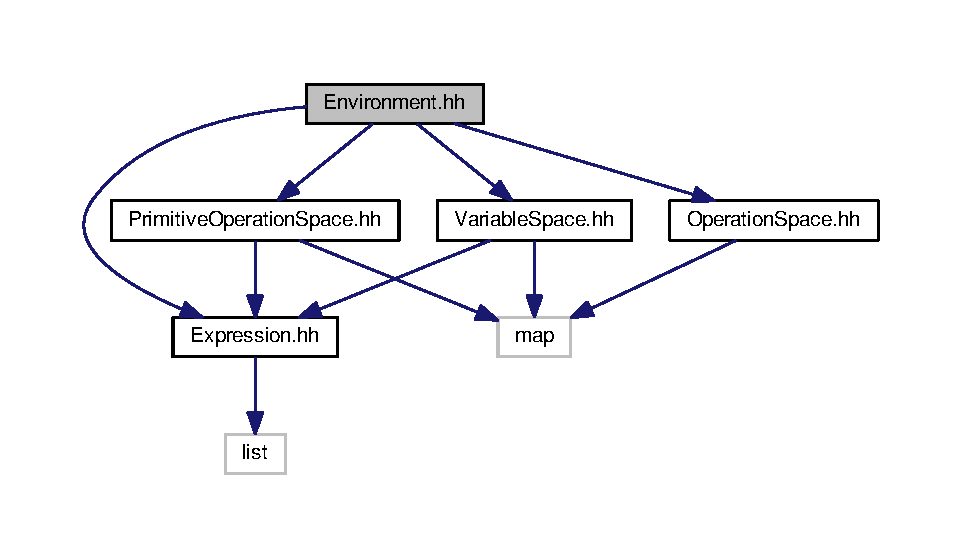
\includegraphics[width=350pt]{_environment_8hh__incl}
\end{center}
\end{figure}
Gráfico de los archivos que directa o indirectamente incluyen a este archivo\+:
\nopagebreak
\begin{figure}[H]
\begin{center}
\leavevmode
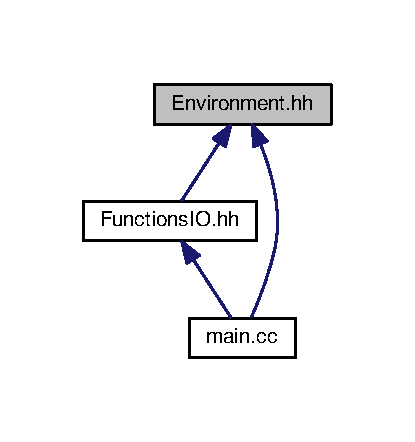
\includegraphics[width=199pt]{_environment_8hh__dep__incl}
\end{center}
\end{figure}
\subsection*{Clases}
\begin{DoxyCompactItemize}
\item 
class \hyperlink{class_environment}{Environment}
\begin{DoxyCompactList}\small\item\em Representa un entorno de ejecución con todas las operaciones primitivas predefinidas, así como con todas las variables y operaciones definidas por el usuario. \end{DoxyCompactList}\end{DoxyCompactItemize}


\subsection{Descripción detallada}
Especificación de la clase \hyperlink{class_environment}{Environment}. 


\hypertarget{_exception_handler_8hh}{}\section{Referencia del Archivo Exception\+Handler.\+hh}
\label{_exception_handler_8hh}\index{Exception\+Handler.\+hh@{Exception\+Handler.\+hh}}


Especificación de la clase \hyperlink{class_exception_handler}{Exception\+Handler}.  


{\ttfamily \#include $<$exception$>$}\\*
Dependencia gráfica adjunta para Exception\+Handler.\+hh\+:\nopagebreak
\begin{figure}[H]
\begin{center}
\leavevmode
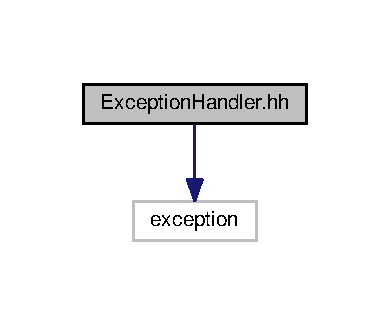
\includegraphics[width=187pt]{_exception_handler_8hh__incl}
\end{center}
\end{figure}
\subsection*{Clases}
\begin{DoxyCompactItemize}
\item 
class \hyperlink{class_exception_handler}{Exception\+Handler}
\begin{DoxyCompactList}\small\item\em Controla la generación de excepciones en caso de fallo de las condiciones básicas de funcionamiento del programa. \end{DoxyCompactList}\end{DoxyCompactItemize}


\subsection{Descripción detallada}
Especificación de la clase \hyperlink{class_exception_handler}{Exception\+Handler}. 


\hypertarget{_expression_8hh}{}\section{Referencia del Archivo Expression.\+hh}
\label{_expression_8hh}\index{Expression.\+hh@{Expression.\+hh}}


Especificación de la clase \hyperlink{class_expression}{Expression}.  


\subsection*{Clases}
\begin{DoxyCompactItemize}
\item 
class \hyperlink{class_expression}{Expression}
\begin{DoxyCompactList}\small\item\em Representa una expresión mediante el resultado de evaluarla, ya sea expresión entera, lista de expresiones enteras o indefinida. \end{DoxyCompactList}\end{DoxyCompactItemize}


\subsection{Descripción detallada}
Especificación de la clase \hyperlink{class_expression}{Expression}. 


\hypertarget{_functions_i_o_8hh}{}\section{Referencia del Archivo Functions\+I\+O.\+hh}
\label{_functions_i_o_8hh}\index{Functions\+I\+O.\+hh@{Functions\+I\+O.\+hh}}


Especificación de las operaciones de lectura/escritura de expresiones.  


Dependencia gráfica adjunta para Functions\+I\+O.\+hh\+:\nopagebreak
\begin{figure}[H]
\begin{center}
\leavevmode
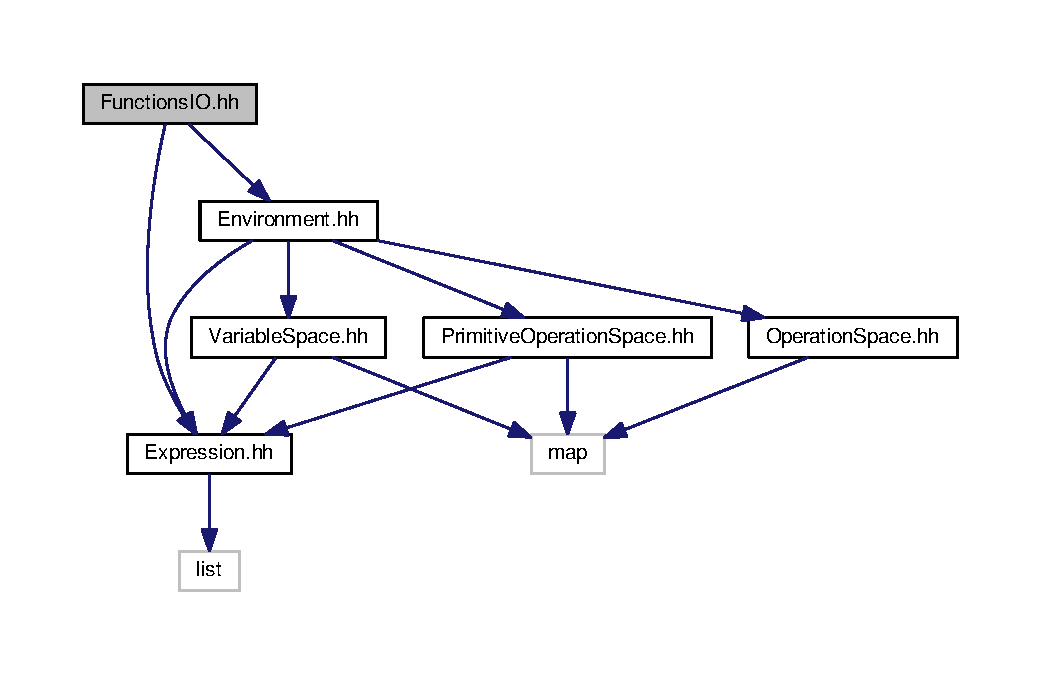
\includegraphics[width=350pt]{_functions_i_o_8hh__incl}
\end{center}
\end{figure}
\subsection*{Funciones}
\begin{DoxyCompactItemize}
\item 
bool \hyperlink{_functions_i_o_8hh_ae6062008fb1c70242c967349d6ee0f9b}{is\+\_\+num} (string str)
\begin{DoxyCompactList}\small\item\em Operación para identicar un número en una cadena de strings. \end{DoxyCompactList}\item 
bool \hyperlink{_functions_i_o_8hh_a9ef0154c2cb7ee5236239fcee8333acb}{is\+\_\+valid} (\hyperlink{class_environment}{Environment} \&env, string str)
\begin{DoxyCompactList}\small\item\em Operación para identificar si los datos introducidos por el canal estandar de entrada son validos. \end{DoxyCompactList}\item 
void \hyperlink{_functions_i_o_8hh_a77ed86fa2fad279d440800e10d0f4a9a}{create\+Local\+Var\+Space} (\hyperlink{class_environment}{Environment} \&env, \hyperlink{class_expression}{Expression} \&exp, string parameters)
\begin{DoxyCompactList}\small\item\em Crea un espacio de variables local. \end{DoxyCompactList}\item 
void \hyperlink{_functions_i_o_8hh_ad4d84fbc6c7e89fb6c14869a204e0913}{evaluate} (\hyperlink{class_environment}{Environment} \&env, \hyperlink{class_expression}{Expression} \&exp)
\begin{DoxyCompactList}\small\item\em Operación de separación de strings. \end{DoxyCompactList}\item 
void \hyperlink{_functions_i_o_8hh_aa35945b371ae9ece372fe0a7c8e97aee}{read\+List} (\hyperlink{class_environment}{Environment} \&env, \hyperlink{class_expression}{Expression} \&exp, \hyperlink{class_input}{Input} \&in)
\begin{DoxyCompactList}\small\item\em Lee una lista de expresiones y las añade a una lista de expresiones de exp. \end{DoxyCompactList}\item 
bool \hyperlink{_functions_i_o_8hh_a52044451543aacd73dad0b1bdfb9c0bd}{check} (\hyperlink{class_environment}{Environment} \&env, \hyperlink{class_input}{Input} \&in)
\begin{DoxyCompactList}\small\item\em Comprueba que una cadena de caracteres sea valida. \end{DoxyCompactList}\item 
void \hyperlink{_functions_i_o_8hh_ae5d92549027ba3619eca48a15b567682}{read\+If} (\hyperlink{class_environment}{Environment} \&env, \hyperlink{class_expression}{Expression} \&exp, \hyperlink{class_input}{Input} \&in)
\begin{DoxyCompactList}\small\item\em Lee la operación if con sus expresiones. \end{DoxyCompactList}\item 
void \hyperlink{_functions_i_o_8hh_acb31c57a06915fe17eee64989f500f0d}{read\+Op} (\hyperlink{class_environment}{Environment} \&env, \hyperlink{class_expression}{Expression} \&exp, \hyperlink{class_input}{Input} \&in)
\begin{DoxyCompactList}\small\item\em Lee una operación primitiva o previamente definida por el usuario. \end{DoxyCompactList}\item 
void \hyperlink{_functions_i_o_8hh_a2b0504402167c389ef8c7de12d41149b}{define\+Var} (\hyperlink{class_environment}{Environment} \&env, string key, \hyperlink{class_input}{Input} \&in)
\begin{DoxyCompactList}\small\item\em Define una variable introducida por el canal estandar de entrada. \end{DoxyCompactList}\item 
void \hyperlink{_functions_i_o_8hh_a39e6424c2643bf6ddf2e5ff8a8c342e9}{define\+Op} (\hyperlink{class_environment}{Environment} \&env, string key, string parameters, \hyperlink{class_input}{Input} \&in)
\begin{DoxyCompactList}\small\item\em Define una operación introducida por el canal estandar de entrada. \end{DoxyCompactList}\item 
void \hyperlink{_functions_i_o_8hh_a65f523a256e113ca2711c3972157df26}{define} (\hyperlink{class_environment}{Environment} \&env, \hyperlink{class_input}{Input} \&in)
\begin{DoxyCompactList}\small\item\em Interpreta si se definirá una variable u operación. \end{DoxyCompactList}\item 
bool \hyperlink{_functions_i_o_8hh_a0c2a0ba0f4fe2dfe26ec14053ce4d408}{read\+Expression} (\hyperlink{class_environment}{Environment} \&env, \hyperlink{class_expression}{Expression} \&exp, \hyperlink{class_input}{Input} \&in)
\begin{DoxyCompactList}\small\item\em Operación de lectura de expresiones. \end{DoxyCompactList}\item 
bool \hyperlink{_functions_i_o_8hh_a10264ecdb3196a71243b69fd4f98c229}{read} (\hyperlink{class_environment}{Environment} \&env, \hyperlink{class_expression}{Expression} \&exp)
\begin{DoxyCompactList}\small\item\em Operación de lectura de expresiones. \end{DoxyCompactList}\end{DoxyCompactItemize}


\subsection{Descripción detallada}
Especificación de las operaciones de lectura/escritura de expresiones. 



\subsection{Documentación de las funciones}
\index{Functions\+I\+O.\+hh@{Functions\+I\+O.\+hh}!is\+\_\+num@{is\+\_\+num}}
\index{is\+\_\+num@{is\+\_\+num}!Functions\+I\+O.\+hh@{Functions\+I\+O.\+hh}}
\subsubsection[{\texorpdfstring{is\+\_\+num(string str)}{is_num(string str)}}]{\setlength{\rightskip}{0pt plus 5cm}bool is\+\_\+num (
\begin{DoxyParamCaption}
\item[{string}]{str}
\end{DoxyParamCaption}
)}\hypertarget{_functions_i_o_8hh_ae6062008fb1c70242c967349d6ee0f9b}{}\label{_functions_i_o_8hh_ae6062008fb1c70242c967349d6ee0f9b}


Operación para identicar un número en una cadena de strings. 

\begin{DoxyPrecond}{Precondición}
{\itshape Cierto} 
\end{DoxyPrecond}
\begin{DoxyPostcond}{Postcondición}
Devuelve cierto si la variable \textquotesingle{}str\textquotesingle{} es un número, falso en caso contrario. 
\end{DoxyPostcond}
\index{Functions\+I\+O.\+hh@{Functions\+I\+O.\+hh}!is\+\_\+valid@{is\+\_\+valid}}
\index{is\+\_\+valid@{is\+\_\+valid}!Functions\+I\+O.\+hh@{Functions\+I\+O.\+hh}}
\subsubsection[{\texorpdfstring{is\+\_\+valid(\+Environment \&env, string str)}{is_valid(Environment &env, string str)}}]{\setlength{\rightskip}{0pt plus 5cm}bool is\+\_\+valid (
\begin{DoxyParamCaption}
\item[{{\bf Environment} \&}]{env, }
\item[{string}]{str}
\end{DoxyParamCaption}
)}\hypertarget{_functions_i_o_8hh_a9ef0154c2cb7ee5236239fcee8333acb}{}\label{_functions_i_o_8hh_a9ef0154c2cb7ee5236239fcee8333acb}


Operación para identificar si los datos introducidos por el canal estandar de entrada son validos. 

\begin{DoxyPrecond}{Precondición}
\textquotesingle{}env\textquotesingle{} es un entorno con variable primitivas previamente inicializadas, str es un string no vacio 
\end{DoxyPrecond}
\begin{DoxyPostcond}{Postcondición}
Devuelve true si str es un parentesis, número, operación definida, variable definida o una primitva. Falso en cualquier otro caso. 
\end{DoxyPostcond}
\index{Functions\+I\+O.\+hh@{Functions\+I\+O.\+hh}!create\+Local\+Var\+Space@{create\+Local\+Var\+Space}}
\index{create\+Local\+Var\+Space@{create\+Local\+Var\+Space}!Functions\+I\+O.\+hh@{Functions\+I\+O.\+hh}}
\subsubsection[{\texorpdfstring{create\+Local\+Var\+Space(\+Environment \&env, Expression \&exp, string parameters)}{createLocalVarSpace(Environment &env, Expression &exp, string parameters)}}]{\setlength{\rightskip}{0pt plus 5cm}void create\+Local\+Var\+Space (
\begin{DoxyParamCaption}
\item[{{\bf Environment} \&}]{env, }
\item[{{\bf Expression} \&}]{exp, }
\item[{string}]{parameters}
\end{DoxyParamCaption}
)}\hypertarget{_functions_i_o_8hh_a77ed86fa2fad279d440800e10d0f4a9a}{}\label{_functions_i_o_8hh_a77ed86fa2fad279d440800e10d0f4a9a}


Crea un espacio de variables local. 

\begin{DoxyPrecond}{Precondición}
\textquotesingle{}env\textquotesingle{} es un entorno con variable primitivas previamente inicializadas, exp una expresion no vacia y parameters los paremtros a definir 
\end{DoxyPrecond}
\begin{DoxyPostcond}{Postcondición}

\end{DoxyPostcond}
\index{Functions\+I\+O.\+hh@{Functions\+I\+O.\+hh}!evaluate@{evaluate}}
\index{evaluate@{evaluate}!Functions\+I\+O.\+hh@{Functions\+I\+O.\+hh}}
\subsubsection[{\texorpdfstring{evaluate(\+Environment \&env, Expression \&exp)}{evaluate(Environment &env, Expression &exp)}}]{\setlength{\rightskip}{0pt plus 5cm}void evaluate (
\begin{DoxyParamCaption}
\item[{{\bf Environment} \&}]{env, }
\item[{{\bf Expression} \&}]{exp}
\end{DoxyParamCaption}
)}\hypertarget{_functions_i_o_8hh_ad4d84fbc6c7e89fb6c14869a204e0913}{}\label{_functions_i_o_8hh_ad4d84fbc6c7e89fb6c14869a204e0913}


Operación de separación de strings. 

\begin{DoxyPrecond}{Precondición}
{\itshape Cierto} 
\end{DoxyPrecond}
\begin{DoxyPostcond}{Postcondición}
\textquotesingle{}str\textquotesingle{} es un string contenido entre espacios o paréntesis en la entrada que se ha leído\+Evalua la expresion exp y retorna su valor en exp
\end{DoxyPostcond}
\begin{DoxyPrecond}{Precondición}
\textquotesingle{}env\textquotesingle{} es un entorno con variable primitivas previamente inicializadas; \textquotesingle{}exp\textquotesingle{} es una expresión a evaluar. 
\end{DoxyPrecond}
\begin{DoxyPostcond}{Postcondición}
Se evalua la expresion \textquotesingle{}exp\textquotesingle{} y se retorna en la misma variable el valor resultante, el cual puede ser\+: una lista de expresiones, un valor o indefinido. 
\end{DoxyPostcond}
\index{Functions\+I\+O.\+hh@{Functions\+I\+O.\+hh}!read\+List@{read\+List}}
\index{read\+List@{read\+List}!Functions\+I\+O.\+hh@{Functions\+I\+O.\+hh}}
\subsubsection[{\texorpdfstring{read\+List(\+Environment \&env, Expression \&exp, Input \&in)}{readList(Environment &env, Expression &exp, Input &in)}}]{\setlength{\rightskip}{0pt plus 5cm}void read\+List (
\begin{DoxyParamCaption}
\item[{{\bf Environment} \&}]{env, }
\item[{{\bf Expression} \&}]{exp, }
\item[{{\bf Input} \&}]{in}
\end{DoxyParamCaption}
)}\hypertarget{_functions_i_o_8hh_aa35945b371ae9ece372fe0a7c8e97aee}{}\label{_functions_i_o_8hh_aa35945b371ae9ece372fe0a7c8e97aee}


Lee una lista de expresiones y las añade a una lista de expresiones de exp. 

\begin{DoxyPrecond}{Precondición}
\textquotesingle{}env\textquotesingle{} es un entorno con variable primitivas previamente inicializadas; \textquotesingle{}exp\textquotesingle{} es una expresión no vacia e input contiene los caracteres a añadir en la lista. 
\end{DoxyPrecond}
\begin{DoxyPostcond}{Postcondición}
Se crea una lista de expresiones en exp, si los valores a añadir son indefinidos, se modifica el valor de la expresion a indefinido. 
\end{DoxyPostcond}
\index{Functions\+I\+O.\+hh@{Functions\+I\+O.\+hh}!check@{check}}
\index{check@{check}!Functions\+I\+O.\+hh@{Functions\+I\+O.\+hh}}
\subsubsection[{\texorpdfstring{check(\+Environment \&env, Input \&in)}{check(Environment &env, Input &in)}}]{\setlength{\rightskip}{0pt plus 5cm}bool check (
\begin{DoxyParamCaption}
\item[{{\bf Environment} \&}]{env, }
\item[{{\bf Input} \&}]{in}
\end{DoxyParamCaption}
)}\hypertarget{_functions_i_o_8hh_a52044451543aacd73dad0b1bdfb9c0bd}{}\label{_functions_i_o_8hh_a52044451543aacd73dad0b1bdfb9c0bd}


Comprueba que una cadena de caracteres sea valida. 

\begin{DoxyPrecond}{Precondición}
\textquotesingle{}env\textquotesingle{} es un entorno con variable primitivas previamente inicializadas; \textquotesingle{}in\textquotesingle{} contiene una cadena de caracteres introducidas por el usuario por el canal estandar de entrada 
\end{DoxyPrecond}
\begin{DoxyPostcond}{Postcondición}
Devuelve cierto si in es una cadena de caracteres valida con parentesis, números, operaciones definidas, variables definidas y/o primitvas, falso en caso contrario. 
\end{DoxyPostcond}
\index{Functions\+I\+O.\+hh@{Functions\+I\+O.\+hh}!read\+If@{read\+If}}
\index{read\+If@{read\+If}!Functions\+I\+O.\+hh@{Functions\+I\+O.\+hh}}
\subsubsection[{\texorpdfstring{read\+If(\+Environment \&env, Expression \&exp, Input \&in)}{readIf(Environment &env, Expression &exp, Input &in)}}]{\setlength{\rightskip}{0pt plus 5cm}void read\+If (
\begin{DoxyParamCaption}
\item[{{\bf Environment} \&}]{env, }
\item[{{\bf Expression} \&}]{exp, }
\item[{{\bf Input} \&}]{in}
\end{DoxyParamCaption}
)}\hypertarget{_functions_i_o_8hh_ae5d92549027ba3619eca48a15b567682}{}\label{_functions_i_o_8hh_ae5d92549027ba3619eca48a15b567682}


Lee la operación if con sus expresiones. 

\begin{DoxyPrecond}{Precondición}
\textquotesingle{}env\textquotesingle{} es un entorno con variable primitivas previamente inicializadas; exp es una expresion inicializada con el operador if, \textquotesingle{}in\textquotesingle{} contiene una cadena de caracteres introducidas por el usuario por el canal estandar de entrada 
\end{DoxyPrecond}
\begin{DoxyPostcond}{Postcondición}
Se evalua la expresion exp y se retorna su resultado en la misma variable, su valor puede ser un valor una lista o indefinido. 
\end{DoxyPostcond}
\index{Functions\+I\+O.\+hh@{Functions\+I\+O.\+hh}!read\+Op@{read\+Op}}
\index{read\+Op@{read\+Op}!Functions\+I\+O.\+hh@{Functions\+I\+O.\+hh}}
\subsubsection[{\texorpdfstring{read\+Op(\+Environment \&env, Expression \&exp, Input \&in)}{readOp(Environment &env, Expression &exp, Input &in)}}]{\setlength{\rightskip}{0pt plus 5cm}void read\+Op (
\begin{DoxyParamCaption}
\item[{{\bf Environment} \&}]{env, }
\item[{{\bf Expression} \&}]{exp, }
\item[{{\bf Input} \&}]{in}
\end{DoxyParamCaption}
)}\hypertarget{_functions_i_o_8hh_acb31c57a06915fe17eee64989f500f0d}{}\label{_functions_i_o_8hh_acb31c57a06915fe17eee64989f500f0d}


Lee una operación primitiva o previamente definida por el usuario. 

\begin{DoxyPrecond}{Precondición}
\textquotesingle{}env\textquotesingle{} es un entorno con variable primitivas previamente inicializadas; exp es una expresion inicializada, \textquotesingle{}in\textquotesingle{} contiene una cadena de caracteres introducidas por el usuario por el canal estandar de entrada 
\end{DoxyPrecond}
\begin{DoxyPostcond}{Postcondición}
Se le asigna un operador op el cual esta en la variable in, a la expresion exp. 
\end{DoxyPostcond}
\index{Functions\+I\+O.\+hh@{Functions\+I\+O.\+hh}!define\+Var@{define\+Var}}
\index{define\+Var@{define\+Var}!Functions\+I\+O.\+hh@{Functions\+I\+O.\+hh}}
\subsubsection[{\texorpdfstring{define\+Var(\+Environment \&env, string key, Input \&in)}{defineVar(Environment &env, string key, Input &in)}}]{\setlength{\rightskip}{0pt plus 5cm}void define\+Var (
\begin{DoxyParamCaption}
\item[{{\bf Environment} \&}]{env, }
\item[{string}]{key, }
\item[{{\bf Input} \&}]{in}
\end{DoxyParamCaption}
)}\hypertarget{_functions_i_o_8hh_a2b0504402167c389ef8c7de12d41149b}{}\label{_functions_i_o_8hh_a2b0504402167c389ef8c7de12d41149b}


Define una variable introducida por el canal estandar de entrada. 

\begin{DoxyPrecond}{Precondición}
env es un entorno con variable primitivas previamente inicializadas; key es el nombre de la variable a definir, \textquotesingle{}in\textquotesingle{} contiene una cadena de caracteres introducidas por el usuario por el canal estandar de entrada 
\end{DoxyPrecond}
\begin{DoxyPostcond}{Postcondición}
Se define una nueva variable con nombre \textquotesingle{}key\textquotesingle{} y el valor esta en la expresion introducida en \textquotesingle{}in\textquotesingle{} por el canal estandar de entrada, esta nueva variable se añade al entorno de environment. Si la evaluacion de la expresion para definir la nueva variable da indefinida, la variable quedara como indefinida. 
\end{DoxyPostcond}
\index{Functions\+I\+O.\+hh@{Functions\+I\+O.\+hh}!define\+Op@{define\+Op}}
\index{define\+Op@{define\+Op}!Functions\+I\+O.\+hh@{Functions\+I\+O.\+hh}}
\subsubsection[{\texorpdfstring{define\+Op(\+Environment \&env, string key, string parameters, Input \&in)}{defineOp(Environment &env, string key, string parameters, Input &in)}}]{\setlength{\rightskip}{0pt plus 5cm}void define\+Op (
\begin{DoxyParamCaption}
\item[{{\bf Environment} \&}]{env, }
\item[{string}]{key, }
\item[{string}]{parameters, }
\item[{{\bf Input} \&}]{in}
\end{DoxyParamCaption}
)}\hypertarget{_functions_i_o_8hh_a39e6424c2643bf6ddf2e5ff8a8c342e9}{}\label{_functions_i_o_8hh_a39e6424c2643bf6ddf2e5ff8a8c342e9}


Define una operación introducida por el canal estandar de entrada. 

\begin{DoxyPrecond}{Precondición}
env es un entorno con variable primitivas previamente inicializadas; key es el nombre de la operacion a definir, \textquotesingle{}in\textquotesingle{} contiene una cadena de caracteres introducidas por el usuario por el canal estandar de entrada, esta cadena contiene la expresión a evaluar. 
\end{DoxyPrecond}
\begin{DoxyPostcond}{Postcondición}
Se define una nueva operación con nombre \textquotesingle{}key\textquotesingle{}, parametros \textquotesingle{}parameters\textquotesingle{} y como valor la cadena introducida por el canal estandar de entrada \textquotesingle{}in\textquotesingle{}, esta nueva operación se añadirá al entorno de environment. No se evalua la expresión al definir la operación, solo se evaluara al utilizar la operación. 
\end{DoxyPostcond}
\index{Functions\+I\+O.\+hh@{Functions\+I\+O.\+hh}!define@{define}}
\index{define@{define}!Functions\+I\+O.\+hh@{Functions\+I\+O.\+hh}}
\subsubsection[{\texorpdfstring{define(\+Environment \&env, Input \&in)}{define(Environment &env, Input &in)}}]{\setlength{\rightskip}{0pt plus 5cm}void define (
\begin{DoxyParamCaption}
\item[{{\bf Environment} \&}]{env, }
\item[{{\bf Input} \&}]{in}
\end{DoxyParamCaption}
)}\hypertarget{_functions_i_o_8hh_a65f523a256e113ca2711c3972157df26}{}\label{_functions_i_o_8hh_a65f523a256e113ca2711c3972157df26}


Interpreta si se definirá una variable u operación. 

\begin{DoxyPrecond}{Precondición}
\textquotesingle{}env\textquotesingle{} es un entorno con variable primitivas previamente inicializadas; \textquotesingle{}in\textquotesingle{} es una cadena con los valores a definir, puede ser la definicion de una variable o de una operación. 
\end{DoxyPrecond}
\begin{DoxyPostcond}{Postcondición}
Se ha creado una varible u operación. Si la expresion es correcta, si es indefinida se creara una exp con el valor indefinido. 
\end{DoxyPostcond}
\index{Functions\+I\+O.\+hh@{Functions\+I\+O.\+hh}!read\+Expression@{read\+Expression}}
\index{read\+Expression@{read\+Expression}!Functions\+I\+O.\+hh@{Functions\+I\+O.\+hh}}
\subsubsection[{\texorpdfstring{read\+Expression(\+Environment \&env, Expression \&exp, Input \&in)}{readExpression(Environment &env, Expression &exp, Input &in)}}]{\setlength{\rightskip}{0pt plus 5cm}bool read\+Expression (
\begin{DoxyParamCaption}
\item[{{\bf Environment} \&}]{env, }
\item[{{\bf Expression} \&}]{exp, }
\item[{{\bf Input} \&}]{in}
\end{DoxyParamCaption}
)}\hypertarget{_functions_i_o_8hh_a0c2a0ba0f4fe2dfe26ec14053ce4d408}{}\label{_functions_i_o_8hh_a0c2a0ba0f4fe2dfe26ec14053ce4d408}


Operación de lectura de expresiones. 

\begin{DoxyPrecond}{Precondición}
\textquotesingle{}env\textquotesingle{} es un entorno con un espacio de operaciones primitivas inicializado con las operaciones primitivas predefinidas; \textquotesingle{}exp\textquotesingle{} es una expresión vacía. 
\end{DoxyPrecond}
\begin{DoxyPostcond}{Postcondición}
Se han leído los datos del canal estándar de entrada y se han asignado a \textquotesingle{}env\textquotesingle{} si eran una definición de una variable u operación o a \textquotesingle{}exp\textquotesingle{} si representaban una expresión evaluable 
\end{DoxyPostcond}
\index{Functions\+I\+O.\+hh@{Functions\+I\+O.\+hh}!read@{read}}
\index{read@{read}!Functions\+I\+O.\+hh@{Functions\+I\+O.\+hh}}
\subsubsection[{\texorpdfstring{read(\+Environment \&env, Expression \&exp)}{read(Environment &env, Expression &exp)}}]{\setlength{\rightskip}{0pt plus 5cm}bool read (
\begin{DoxyParamCaption}
\item[{{\bf Environment} \&}]{env, }
\item[{{\bf Expression} \&}]{exp}
\end{DoxyParamCaption}
)}\hypertarget{_functions_i_o_8hh_a10264ecdb3196a71243b69fd4f98c229}{}\label{_functions_i_o_8hh_a10264ecdb3196a71243b69fd4f98c229}


Operación de lectura de expresiones. 

\begin{DoxyPrecond}{Precondición}
\textquotesingle{}env\textquotesingle{} es un entorno con un espacio de operaciones primitivas inicializado con las operaciones primitivas predefinidas; \textquotesingle{}exp\textquotesingle{} es una expresión vacía 
\end{DoxyPrecond}
\begin{DoxyPostcond}{Postcondición}
Se han leído los datos del canal estándar de entrada y se han asignado a \textquotesingle{}env\textquotesingle{} si eran una definición de una variable o operación o a \textquotesingle{}exp\textquotesingle{} si representaban una expresión evaluable 
\end{DoxyPostcond}

\hypertarget{main_8cc}{}\section{Referencia del Archivo main.\+cc}
\label{main_8cc}\index{main.\+cc@{main.\+cc}}


Programa principal para la calculadora de expresiones aritméticas.  


{\ttfamily \#include $<$iostream$>$}\\*
{\ttfamily \#include \char`\"{}Functions\+I\+O.\+hh\char`\"{}}\\*
{\ttfamily \#include \char`\"{}Environment.\+hh\char`\"{}}\\*
{\ttfamily \#include \char`\"{}Expression.\+hh\char`\"{}}\\*
Dependencia gráfica adjunta para main.\+cc\+:\nopagebreak
\begin{figure}[H]
\begin{center}
\leavevmode
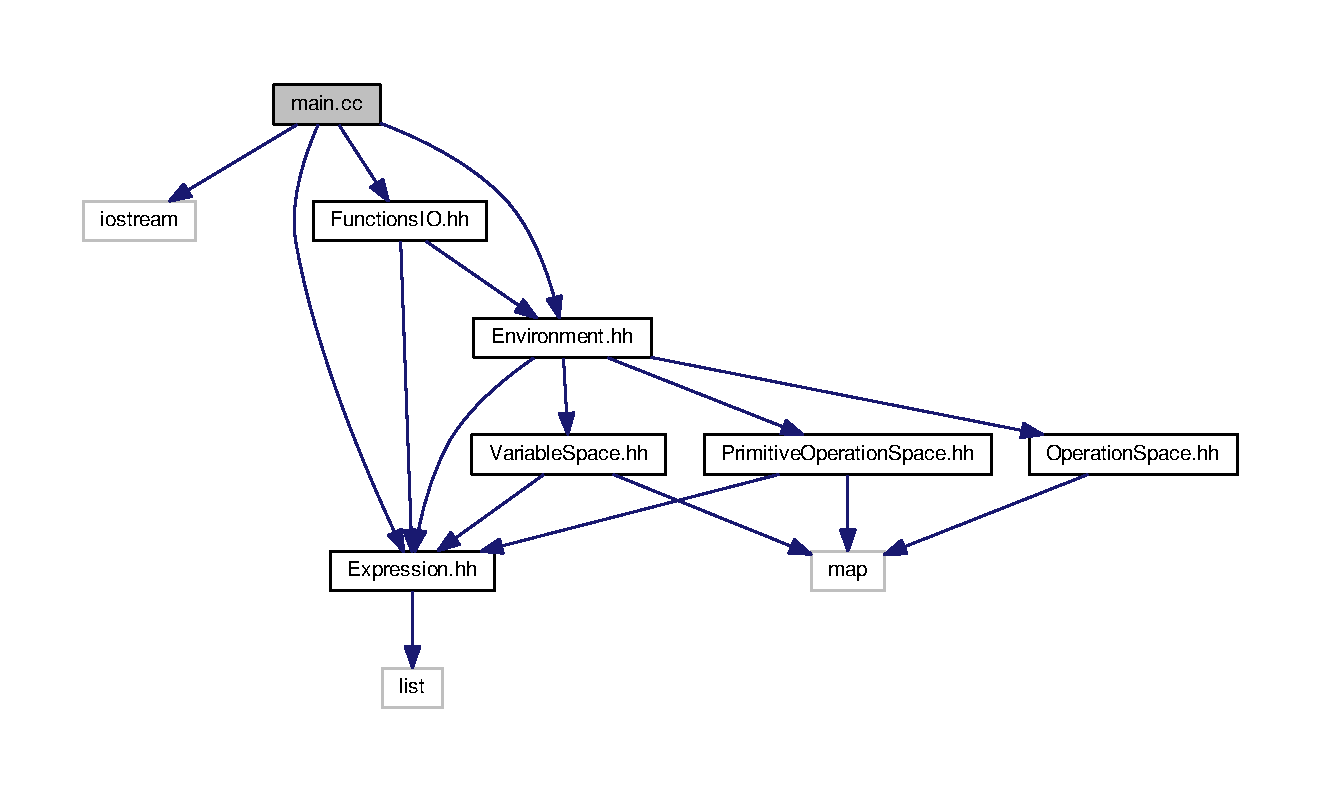
\includegraphics[width=350pt]{main_8cc__incl}
\end{center}
\end{figure}
\subsection*{Funciones}
\begin{DoxyCompactItemize}
\item 
int \hyperlink{main_8cc_ae66f6b31b5ad750f1fe042a706a4e3d4}{main} ()\hypertarget{main_8cc_ae66f6b31b5ad750f1fe042a706a4e3d4}{}\label{main_8cc_ae66f6b31b5ad750f1fe042a706a4e3d4}

\begin{DoxyCompactList}\small\item\em Programa principal para la calculadora de expresiones aritméticas. \end{DoxyCompactList}\end{DoxyCompactItemize}


\subsection{Descripción detallada}
Programa principal para la calculadora de expresiones aritméticas. 


\hypertarget{_operation_space_8hh}{}\section{Referencia del Archivo Operation\+Space.\+hh}
\label{_operation_space_8hh}\index{Operation\+Space.\+hh@{Operation\+Space.\+hh}}


Especificación de la clase \hyperlink{class_operation_space}{Operation\+Space}.  


{\ttfamily \#include $<$map$>$}\\*
Dependencia gráfica adjunta para Operation\+Space.\+hh\+:
\nopagebreak
\begin{figure}[H]
\begin{center}
\leavevmode
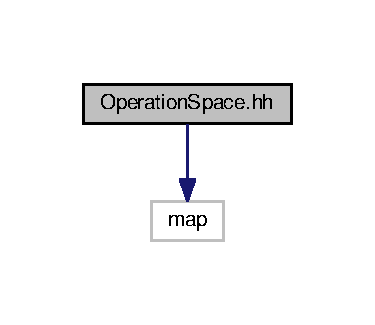
\includegraphics[width=180pt]{_operation_space_8hh__incl}
\end{center}
\end{figure}
Gráfico de los archivos que directa o indirectamente incluyen a este archivo\+:
\nopagebreak
\begin{figure}[H]
\begin{center}
\leavevmode
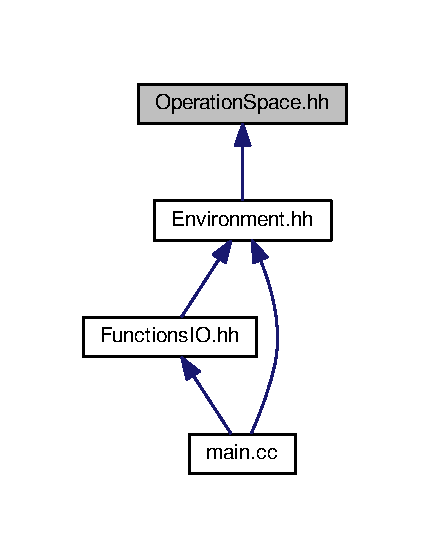
\includegraphics[width=207pt]{_operation_space_8hh__dep__incl}
\end{center}
\end{figure}
\subsection*{Clases}
\begin{DoxyCompactItemize}
\item 
class \hyperlink{class_operation_space}{Operation\+Space}
\begin{DoxyCompactList}\small\item\em Representa un espacio de operaciones definidas por el usuario en forma de mapa de variables. \end{DoxyCompactList}\end{DoxyCompactItemize}


\subsection{Descripción detallada}
Especificación de la clase \hyperlink{class_operation_space}{Operation\+Space}. 


\hypertarget{_primitive_operation_space_8hh}{}\section{Referencia del Archivo Primitive\+Operation\+Space.\+hh}
\label{_primitive_operation_space_8hh}\index{Primitive\+Operation\+Space.\+hh@{Primitive\+Operation\+Space.\+hh}}


Especificación de la clase \hyperlink{class_primitive_operation_space}{Primitive\+Operation\+Space}.  


{\ttfamily \#include $<$map$>$}\\*
{\ttfamily \#include \char`\"{}Expression.\+hh\char`\"{}}\\*
Dependencia gráfica adjunta para Primitive\+Operation\+Space.\+hh\+:\nopagebreak
\begin{figure}[H]
\begin{center}
\leavevmode
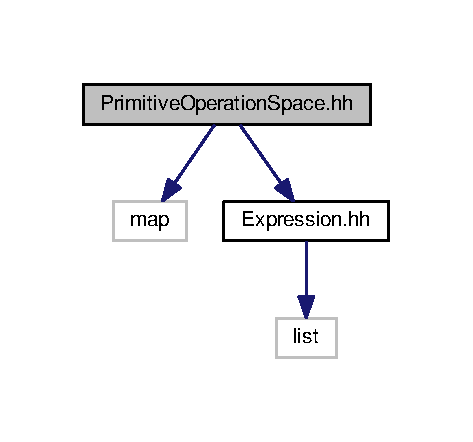
\includegraphics[width=227pt]{_primitive_operation_space_8hh__incl}
\end{center}
\end{figure}
Gráfico de los archivos que directa o indirectamente incluyen a este archivo\+:\nopagebreak
\begin{figure}[H]
\begin{center}
\leavevmode
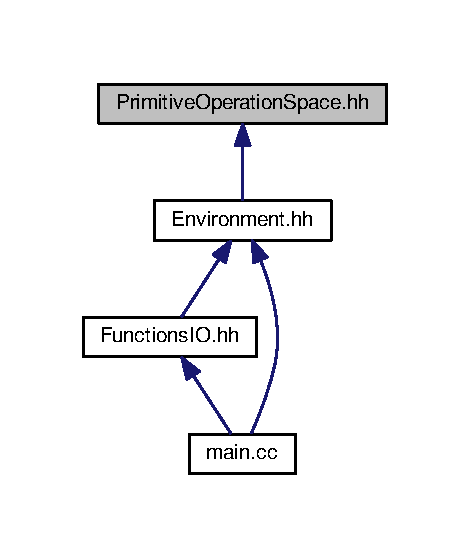
\includegraphics[width=226pt]{_primitive_operation_space_8hh__dep__incl}
\end{center}
\end{figure}
\subsection*{Clases}
\begin{DoxyCompactItemize}
\item 
class \hyperlink{class_primitive_operation_space}{Primitive\+Operation\+Space}
\begin{DoxyCompactList}\small\item\em Representa un espacio de operaciones primitivas predefinidas en forma de mapa de operaciones. \end{DoxyCompactList}\end{DoxyCompactItemize}


\subsection{Descripción detallada}
Especificación de la clase \hyperlink{class_primitive_operation_space}{Primitive\+Operation\+Space}. 


\hypertarget{_variable_space_8hh}{}\section{Referencia del Archivo Variable\+Space.\+hh}
\label{_variable_space_8hh}\index{Variable\+Space.\+hh@{Variable\+Space.\+hh}}


Especificación de la clase \hyperlink{class_variable_space}{Variable\+Space}.  


{\ttfamily \#include $<$map$>$}\\*
{\ttfamily \#include \char`\"{}Expression.\+hh\char`\"{}}\\*
Dependencia gráfica adjunta para Variable\+Space.\+hh\+:\nopagebreak
\begin{figure}[H]
\begin{center}
\leavevmode
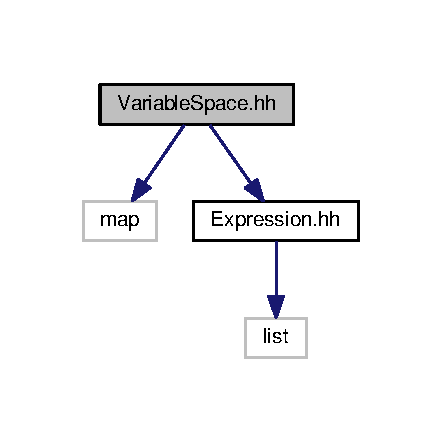
\includegraphics[width=212pt]{_variable_space_8hh__incl}
\end{center}
\end{figure}
Gráfico de los archivos que directa o indirectamente incluyen a este archivo\+:\nopagebreak
\begin{figure}[H]
\begin{center}
\leavevmode
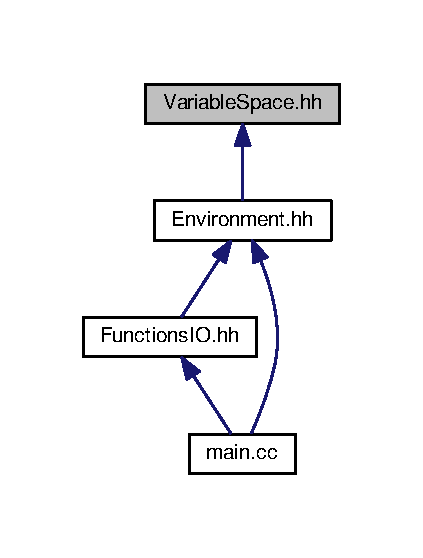
\includegraphics[width=203pt]{_variable_space_8hh__dep__incl}
\end{center}
\end{figure}
\subsection*{Clases}
\begin{DoxyCompactItemize}
\item 
class \hyperlink{class_variable_space}{Variable\+Space}
\begin{DoxyCompactList}\small\item\em Representa un espacio de variables definidas por el usuario en forma de mapa de variables. \end{DoxyCompactList}\end{DoxyCompactItemize}


\subsection{Descripción detallada}
Especificación de la clase \hyperlink{class_variable_space}{Variable\+Space}. 


%--- End generated contents ---

% Index
\backmatter
\newpage
\phantomsection
\clearemptydoublepage
\addcontentsline{toc}{chapter}{Índice}
\printindex

\end{document}
